% AI-Powered Data Analytics & Visualization Platform - CSE-638 capstone report.
% Build:  latexmk -pdf REPORT.tex      (or: pdflatex REPORT.tex, twice)
% Figures are committed under report/figures/ and regenerated from the repo root by
%   python -m scripts.export_report_assets
\documentclass[11pt,a4paper]{article}

\usepackage[T1]{fontenc}
\usepackage[utf8]{inputenc}
\usepackage{lmodern}
% 1.9cm rather than the usual 2.2: the brief caps the report at 20 pages and the
% screenshots are worth more than the whitespace.
\usepackage[margin=1.9cm]{geometry}
\usepackage{microtype}
\usepackage{graphicx}
\usepackage{booktabs}
\usepackage{longtable}
\usepackage{array}
\usepackage{multirow}
\usepackage{tabularx}
\usepackage{amssymb}
\usepackage{xcolor}
\usepackage{listings}
\usepackage{caption}
\usepackage{enumitem}
\usepackage{fancyhdr}
\usepackage{tikz}
\usetikzlibrary{arrows.meta,positioning,fit,backgrounds}
\usepackage[hidelinks]{hyperref}

\graphicspath{{figures/}}

\definecolor{brand}{HTML}{2A78D6}
\definecolor{ink}{HTML}{0B0B0B}
\definecolor{muted}{HTML}{52514E}
\definecolor{rule}{HTML}{E1E0D9}
\definecolor{surface}{HTML}{F9F9F7}
\definecolor{loss}{HTML}{D03B3B}

\hypersetup{colorlinks=true,linkcolor=brand,urlcolor=brand,citecolor=brand}

\captionsetup{font=small,labelfont={bf,color=brand}}

\pagestyle{fancy}
\fancyhf{}
\fancyhead[L]{\small\color{muted}AI-Powered Data Analytics \& Visualization Platform}
\fancyhead[R]{\small\color{muted}\thepage}
\renewcommand{\headrulewidth}{0.4pt}

\lstdefinestyle{code}{
  basicstyle=\ttfamily\scriptsize,
  backgroundcolor=\color{surface},
  frame=leftline,
  framerule=2pt,
  rulecolor=\color{rule},
  framesep=6pt,
  xleftmargin=8pt,
  breaklines=true,
  columns=fullflexible,
  keepspaces=true,
  showstringspaces=false,
  keywordstyle=\color{brand}\bfseries,
  commentstyle=\color{muted}\itshape,
  stringstyle=\color{loss},
}
\lstset{style=code}

% Tighter lists - the report is page-limited.
\setlist{itemsep=1pt,parsep=0pt,topsep=3pt}

% Fourteen figures in twenty pages. Left at their defaults, LaTeX would rather push
% a float to the next page than fill 90% of this one, and the report bleeds pages to
% whitespace. These let a float sit on a page that is nearly full.
\setlength{\textfloatsep}{10pt plus 2pt minus 2pt}
\setlength{\floatsep}{10pt plus 2pt minus 2pt}
\setlength{\intextsep}{10pt plus 2pt minus 2pt}
\renewcommand{\topfraction}{0.92}
\renewcommand{\bottomfraction}{0.9}
\renewcommand{\textfraction}{0.06}
\renewcommand{\floatpagefraction}{0.88}
\captionsetup{skip=4pt}

\newcommand{\note}[1]{\textcolor{muted}{\small #1}}

\begin{document}

% =====================================================================
% 1. TITLE PAGE
% =====================================================================
\begin{titlepage}
\centering
\vspace*{2.2cm}

{\color{brand}\rule{\textwidth}{2pt}}
\vspace{0.8cm}

{\Huge\bfseries AI-Powered Data Analytics\\[0.25cm] \& Visualization Platform\par}
\vspace{0.7cm}

{\large Natural-language analytics over e-commerce transactions\\ using a locally hosted 4B-parameter language model\par}
\vspace{0.4cm}

{\color{brand}\rule{\textwidth}{2pt}}
\vspace{1.4cm}

\begin{tabular}{@{}ll@{}}
\textbf{Course}         & CSE-638 Deep Learning --- MSc Computer Science \& Engineering \\[2pt]
\textbf{Group}          & Team No.\ 5 \\[2pt]
\textbf{Dataset}        & Global E-Commerce Sales (Superstore) --- 9,994 order line items \\[2pt]
\textbf{Language model} & Gemma 4 E4B (4B effective params), served locally via LM Studio \\[2pt]
\textbf{GitHub}         & \url{https://github.com/spaul571/ai-analytics-platform} \\[2pt]
\textbf{Live demo}      & Streamlit Community Cloud --- see \S\ref{sec:deploy} \\[2pt]
\textbf{Submitted}      & 17 July 2026 \\
\end{tabular}

\vspace{1.2cm}
{\large\bfseries Team members\par}
\vspace{0.35cm}

\begin{tabular}{@{}ll@{}}
\toprule
\textbf{Name} & \textbf{Student ID} \\
\midrule
Shrikanta Paul        & 261-25-017 \\
Md.\ Nurol Amin       & 261-25-021 \\
Animesh Dey           & 261-25-019 \\
Kazi Meherunnesa Eva  & 261-25-033 \\
Fardin Ahmed Alvi     & 261-25-034 \\
Anika Tahsin Prova    & 252-25-016 \\
\bottomrule
\end{tabular}

\vfill
\note{Every figure in this report is regenerated by \texttt{python -m scripts.export\_report\_assets}.
Every number quoted is reproduced by the acceptance scripts in \texttt{scripts/}.}
\end{titlepage}

% =====================================================================
% 2. ABSTRACT
% =====================================================================
\section{Abstract}

We built an end-to-end analytics platform that answers plain-English questions about
9,994 e-commerce order lines by generating, safely executing, and narrating pandas
code. The intelligence layer is \textbf{Gemma 4 E4B}, a 4-billion-parameter model
running locally in LM Studio --- chosen over a hosted API to eliminate cost, rate
limits, and data egress.

The system comprises a pandas data layer (sub-5\,ms filtered aggregations, 79\%
memory reduction via categorical downcasting), a three-phase natural-language query
pipeline guarded by a three-layer execution sandbox, an eight-chart Plotly dashboard
with rule-based automatic chart selection, and two advanced features: Isolation
Forest anomaly detection and a ReAct tool-calling agent that reaches an external
public-holiday API to answer questions the dataset alone cannot.

On a 10-question benchmark scored against hand-written ground truth, text-to-code
accuracy improved from \textbf{5/10 to 10/10} across three iterations. Critically,
\textbf{none of that gain came from a larger model} --- it came from three diagnosed
defects: a JSON-escaping interaction that corrupted generated code, a missing
few-shot pattern, and a defence-in-depth bug in which our own sandbox's two layers
disagreed. The project's central finding is that small-model reliability is an
\emph{engineering} problem, not a capacity problem.

\vspace{0.3cm}
\noindent\textbf{Keywords:} text-to-SQL, local LLM inference, sandboxed code
execution, prompt engineering, anomaly detection, ReAct agents

% =====================================================================
% 3. INTRODUCTION
% =====================================================================
\section{Introduction}

\subsection{Problem motivation}

Analytics tooling has an access problem. The people who most need answers from data
--- category managers, regional leads, finance --- are rarely the people who can
write \texttt{df.groupby(\allowbreak'Sub-Category')\allowbreak['Profit']\allowbreak.sum()}. Every
question therefore queues behind an analyst, and questions that would take ten seconds
to answer take two days to ask.

Large language models collapse that queue by translating natural language into
executable queries. But most demonstrations of this rely on frontier hosted models,
which introduces per-query cost, rate limits, and --- for any business with
commercially sensitive data --- an unacceptable requirement to ship that data to a
third party.

This project asks a narrower and more practical question: \textbf{can a
4-billion-parameter model running on a single consumer GPU do this reliably enough to
be useful?} The answer we arrive at is yes, but only with engineering that a frontier
model would not require.

\subsection{Dataset}
\label{sec:dataset}

The \textbf{Global E-Commerce Sales (Superstore)} dataset: 9,994 retail order line
items across four years (2014--2017), 21 source columns.

\begin{center}
\begin{tabular}{@{}ll@{}}
\toprule
\textbf{Property} & \textbf{Value} \\
\midrule
Rows              & 9,994 \\
Source columns    & 21 \\
Derived columns   & 3 (\texttt{Order Year}, \texttt{Order Month}, \texttt{Shipping Days}) \\
Date range        & 2014-01-03 $\rightarrow$ 2017-12-30 \\
Completeness      & 100.00\% \\
Duplicate rows    & 0 \\
Geography         & United States, 49 states, 4 regions \\
\bottomrule
\end{tabular}
\end{center}

Each row is one product line within a customer order. \texttt{Sales} is gross
revenue; \texttt{Profit} is net margin and \textbf{can be negative} --- a
deliberately chosen property, because a signed metric forces genuine design decisions
throughout (diverging colour scales, aggregate-then-filter query semantics,
loss-focused anomaly detection) that an all-positive dataset would let us dodge.

\paragraph{Why this dataset, given a 4B model.} The selection was driven by the
model, not the other way round. Superstore's column names are unambiguous English
(\texttt{Sales}, \texttt{Profit}, \texttt{Region}), and virtually every analytical
question reduces to a single \texttt{groupby} --- which is precisely the shape a small
model emits reliably. The alternatives were rejected on the same grounds: the Stack
Overflow survey stores languages as a semicolon-delimited multi-select requiring
\texttt{.str.split().explode()} chains; the NYC taxi and S\&P 500 datasets require
rolling-window and temporal binning logic. Each of those is a code shape a 4B model
gets wrong far more often than it gets a plain \texttt{groupby} right.

\subsection{Analytical goals}

\begin{enumerate}[leftmargin=*]
\item Answer arbitrary natural-language questions with executable, verifiable code.
\item Surface the profitability structure hidden beneath headline revenue.
\item Detect and explain anomalous transactions.
\item Do all of it with a model that runs locally and costs nothing per query.
\end{enumerate}

% =====================================================================
% 4. SYSTEM ARCHITECTURE
% =====================================================================
\section{System Architecture}

\begin{figure}[htbp]
\centering
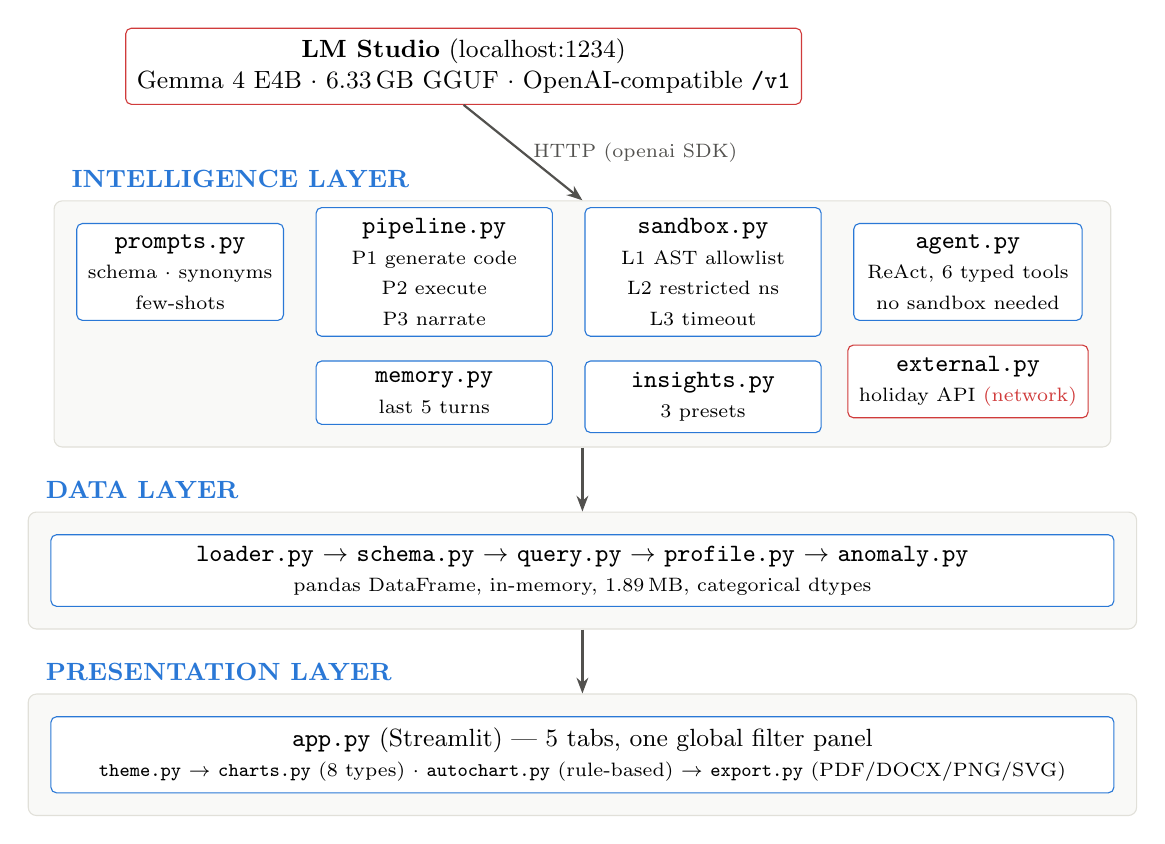
\begin{tikzpicture}[
  font=\small,
  layer/.style={draw=rule,fill=surface,rounded corners=3pt,inner sep=8pt},
  box/.style={draw=brand,fill=white,rounded corners=2pt,align=center,inner sep=4pt,minimum height=8mm},
  lbl/.style={color=brand,font=\small\bfseries},
  flow/.style={-{Stealth[length=2mm]},draw=muted,thick},
]

% --- LLM
\node[box,draw=loss,minimum width=6.6cm] (llm)
  {\textbf{LM Studio} (localhost:1234)\\ Gemma 4 E4B $\cdot$ 6.33\,GB GGUF $\cdot$ OpenAI-compatible \texttt{/v1}};

% --- intelligence layer
\node[box,below=1.5cm of llm.south,xshift=-3.6cm,minimum width=2.6cm] (prompts) {\texttt{prompts.py}\\\scriptsize schema $\cdot$ synonyms\\\scriptsize few-shots};
\node[box,right=4mm of prompts,minimum width=3.0cm] (pipe) {\texttt{pipeline.py}\\\scriptsize P1 generate code\\\scriptsize P2 execute\\\scriptsize P3 narrate};
\node[box,right=4mm of pipe,minimum width=3.0cm] (sand) {\texttt{sandbox.py}\\\scriptsize L1 AST allowlist\\\scriptsize L2 restricted ns\\\scriptsize L3 timeout};
\node[box,right=4mm of sand,minimum width=2.9cm] (agent) {\texttt{agent.py}\\\scriptsize ReAct, 6 typed tools\\\scriptsize no sandbox needed};
\node[box,below=3mm of pipe,minimum width=3.0cm] (mem) {\texttt{memory.py}\\\scriptsize last 5 turns};
\node[box,below=3mm of sand,minimum width=3.0cm] (ins) {\texttt{insights.py}\\\scriptsize 3 presets};
\node[box,below=3mm of agent,minimum width=2.9cm,draw=loss] (ext) {\texttt{external.py}\\\scriptsize holiday API \textcolor{loss}{(network)}};

\begin{scope}[on background layer]
\node[layer,fit=(prompts)(agent)(ext)(mem)] (intel) {};
\end{scope}
\node[lbl,anchor=south west] at ([xshift=3pt,yshift=1pt]intel.north west) {INTELLIGENCE LAYER};

% --- data layer
\node[box,below=1.1cm of intel.south,minimum width=13.5cm] (data)
  {\texttt{loader.py} $\rightarrow$ \texttt{schema.py} $\rightarrow$ \texttt{query.py} $\rightarrow$ \texttt{profile.py} $\rightarrow$ \texttt{anomaly.py}\\
   \scriptsize pandas DataFrame, in-memory, 1.89\,MB, categorical dtypes};
\begin{scope}[on background layer]
\node[layer,fit=(data)] (datal) {};
\end{scope}
\node[lbl,anchor=south west] at ([xshift=3pt,yshift=1pt]datal.north west) {DATA LAYER};

% --- presentation
\node[box,below=1.1cm of datal.south,minimum width=13.5cm] (pres)
  {\texttt{app.py} (Streamlit) --- 5 tabs, one global filter panel\\
   \scriptsize \texttt{theme.py} $\rightarrow$ \texttt{charts.py} (8 types) $\cdot$ \texttt{autochart.py} (rule-based) $\rightarrow$ \texttt{export.py} (PDF/DOCX/PNG/SVG)};
\begin{scope}[on background layer]
\node[layer,fit=(pres)] (presl) {};
\end{scope}
\node[lbl,anchor=south west] at ([xshift=3pt,yshift=1pt]presl.north west) {PRESENTATION LAYER};

\draw[flow] (llm.south) -- node[right,font=\scriptsize,color=muted] {HTTP (openai SDK)} (intel.north);
\draw[flow] (intel.south) -- (datal.north);
\draw[flow] (datal.south) -- (presl.north);
\end{tikzpicture}
\caption{Data flow from the local model down to the browser. Every layer is a plain
Python module; the only two components that leave the machine are the LM Studio
endpoint and the agent's holiday lookup (\S\ref{sec:agent}).}
\end{figure}

\paragraph{Where each requirement lives.} Every claim in this report is reproducible
by a script in the repository rather than by taking our word for it.

\begin{center}
\small
\begin{tabularx}{\textwidth}{@{}llX@{}}
\toprule
\textbf{Task} & \textbf{Module} & \textbf{Reproduce it with} \\
\midrule
A1 Ingestion, schema   & \texttt{data/loader.py}, \texttt{data/schema.py} & \multirow{4}{*}{\texttt{scripts/check\_task\_a.py}} \\
A2 Query engine        & \texttt{data/query.py}          & \\
A3 Quality profiling   & \texttt{data/profile.py}        & \\
A4 Performance         & ---                             & \\
\addlinespace
B1 Prompt design       & \texttt{llm/prompts.py}         & \multirow{5}{*}{\texttt{scripts/check\_task\_b.py}} \\
B2 Text-to-code        & \texttt{llm/pipeline.py}, \texttt{llm/sandbox.py} & \\
B3 Insights            & \texttt{llm/insights.py}        & \\
B4 Context             & \texttt{llm/memory.py}          & \\
B5 Reliability         & \texttt{llm/client.py}          & \\
\addlinespace
C1 Dashboard           & \texttt{app.py}                 & \multirow{4}{*}{\texttt{scripts/check\_task\_c.py}} \\
C2 Chart suite         & \texttt{viz/charts.py}, \texttt{viz/theme.py} & \\
C3 AI-driven charts    & \texttt{viz/autochart.py}       & \\
C4 Export              & \texttt{viz/export.py}, \texttt{viz/browserless.py} & \\
\addlinespace
D3 Anomaly detection   & \texttt{advanced/anomaly.py}    & \multirow{2}{*}{\texttt{scripts/check\_task\_d.py}} \\
D4 ReAct agent         & \texttt{advanced/agent.py}, \texttt{data/external.py} & \\
\bottomrule
\end{tabularx}
\end{center}

\paragraph{Data flow for one natural-language question.}
\begin{enumerate}[leftmargin=*]
\item User types \emph{``Which sub-categories are losing us money?''}
\item \texttt{prompts.py} assembles: schema table + 37-entry synonym map + 6 few-shot
      examples + last 5 conversation turns.
\item \textbf{Phase 1} --- Gemma returns:
\begin{lstlisting}
{"code": "totals = df.groupby('Sub-Category', observed=True)['Profit'].sum()
          \nresult = totals[totals < 0].sort_values()"}
\end{lstlisting}
\item \textbf{Phase 2} --- \texttt{sandbox.py} validates the AST, then executes in a
      restricted namespace with a 10\,s budget. On failure, the exception is fed back
      for exactly one auto-retry.
\item \textbf{Phase 3} --- Gemma narrates the \emph{result table only} (never the raw
      DataFrame), which is what prevents it inventing numbers.
\item \texttt{autochart.py} picks a chart type from the result's \emph{shape},
      renders it, and asks Gemma for a one-sentence caption.
\end{enumerate}

\subsection{Deployment --- and the constraint that shaped it}
\label{sec:deploy}

The brief asks for two things that pull against each other. M6 requires a \emph{``live
demo from GitHub deployment''}, and the brief's \S7.3 prohibits \emph{``hardcoding results or
faking LLM responses --- all AI calls must be live during the demo.''}

Our model runs in LM Studio on a local machine. \textbf{A cloud-hosted frontend cannot
reach \texttt{localhost:1234} on a laptop.} Deploying the app to Streamlit Community
Cloud in the obvious way therefore produces an application with no language model at
all: the dashboard renders, the charts draw from the committed CSV, and every
natural-language question fails. The three ways out are to fake the responses
(prohibited), to abandon the local model for a paid hosted API (which discards the
cost and privacy argument in \S\ref{sec:model}), or to give the local model a public
address. We did the third.

\begin{figure}[htbp]
\centering
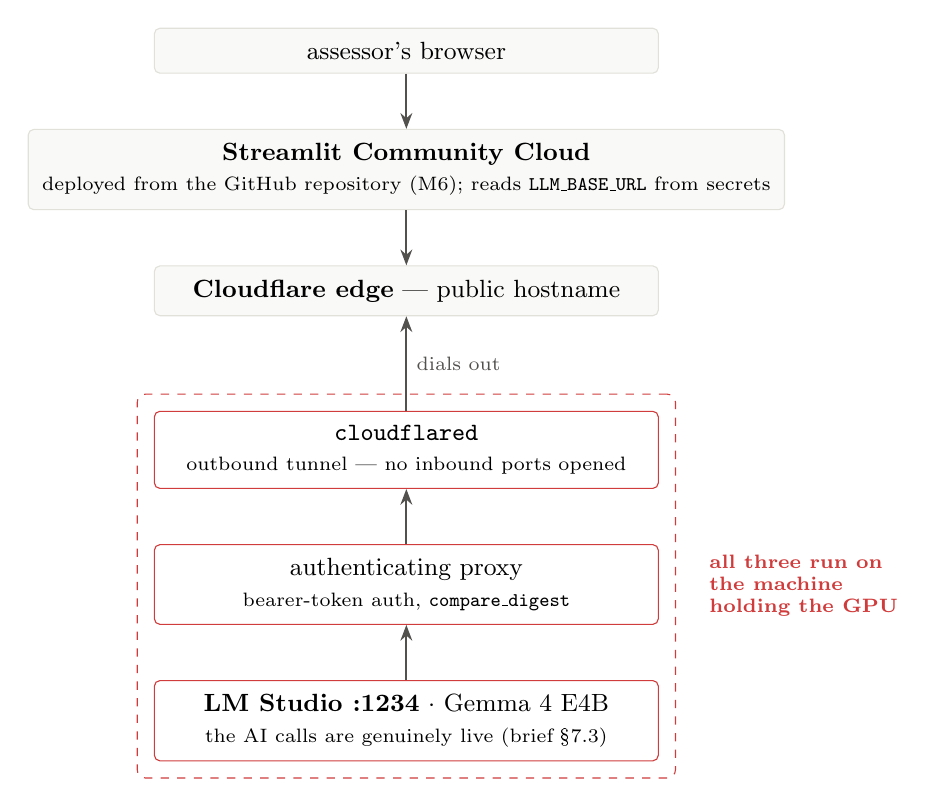
\begin{tikzpicture}[
  font=\small,
  node distance=7mm,
  box/.style={draw=rule,fill=surface,rounded corners=2pt,align=center,inner sep=5pt,minimum width=6.4cm},
  gpu/.style={draw=loss,fill=white,rounded corners=2pt,align=center,inner sep=5pt,minimum width=6.4cm},
  flow/.style={-{Stealth[length=2mm]},draw=muted,thick},
]
\node[box] (browser) {assessor's browser};
\node[box,below=of browser] (cloud) {\textbf{Streamlit Community Cloud}\\\scriptsize deployed from the GitHub repository (M6); reads \texttt{LLM\_BASE\_URL} from secrets};
\node[box,below=of cloud] (edge) {\textbf{Cloudflare edge} --- public hostname};
\node[gpu,below=12mm of edge] (tunnel) {\texttt{cloudflared}\\\scriptsize outbound tunnel --- no inbound ports opened};
\node[gpu,below=of tunnel] (proxy) {authenticating proxy\\\scriptsize bearer-token auth, \texttt{compare\_digest}};
\node[gpu,below=of proxy] (lms) {\textbf{LM Studio :1234} $\cdot$ Gemma 4 E4B\\\scriptsize the AI calls are genuinely live (brief \S7.3)};
% The proxy is local operations tooling and is not published with the application,
% so it is described here rather than cited by a path a reader cannot open.

\draw[flow] (browser) -- (cloud);
\draw[flow] (cloud) -- (edge);
\draw[flow] (tunnel) -- node[right,font=\scriptsize,color=muted] {dials out} (edge);
\draw[flow] (proxy) -- (tunnel);
\draw[flow] (lms) -- (proxy);

\node[draw=loss,dashed,rounded corners=3pt,fit=(tunnel)(proxy)(lms),inner sep=6pt] (gpubox) {};
\node[font=\scriptsize\bfseries,color=loss,anchor=west] at ([xshift=3mm]gpubox.east)
  {\begin{tabular}{@{}l@{}}all three run on\\the machine\\holding the GPU\end{tabular}};
\end{tikzpicture}
\caption{The deployment topology. The tunnel dials outward, so no inbound port is
opened and campus wifi client-isolation cannot break it.}
\end{figure}

Two properties of this topology are worth stating explicitly, because both were design
decisions rather than accidents.

\paragraph{The tunnel is outbound.} \texttt{cloudflared} dials out to Cloudflare;
nothing dials in to us. No port forwarding and no firewall exception is required, and
--- the reason this matters on presentation day --- university networks that isolate
wifi clients from one another cannot break it, because Streamlit Cloud talks to
Cloudflare, never to our laptop. The laptop needs ordinary outbound internet and
nothing more.

\paragraph{The authenticating proxy is not optional.} LM Studio's OpenAI-compatible
server has no authentication of any kind: anything that can reach port 1234 can run
inference and enumerate the loaded models. That is harmless on \texttt{localhost} and
unacceptable the moment the port acquires a public hostname. A small authenticating
proxy is what the tunnel actually exposes, and it rejects any request whose
\texttt{Authorization} header does not carry the expected bearer token, comparing with
\texttt{secrets.compare\_digest} so the token cannot be recovered from response timing.
It refuses to start at all if no token is configured, because an unauthenticated proxy
would silently defeat its own purpose.

The application code required \textbf{no changes} to work through this. The OpenAI SDK
already transmits its \texttt{api\_key} as \texttt{Authorization: Bearer <key>}, which
is precisely what the proxy checks, so setting \texttt{LLM\_API\_KEY} equal to the
proxy's token is the entire integration. This is a dividend of having put every
machine-dependent value in \texttt{config.py} from the start.

\subsection{The container that segfaulted twice}
\label{sec:segfault}

Deploying to Streamlit Cloud produced two failures that never occur locally, and both
are worth recording because both were caused by the \emph{environment}, not the code.

\textbf{First, the container died on boot with SIGSEGV.} The cause was
\texttt{packages.txt}, which asked apt for Chromium so that kaleido could rasterise
charts for the exports (\S\ref{sec:export}). That request pulled 294 packages and
989\,MB --- the whole GTK, Mesa and systemd stack --- and among them Debian's own
\texttt{python3.13} and \texttt{libpython3.13-stdlib}. Streamlit Cloud runs the app
from a venv on Python 3.13.14, so apt dropped a \emph{different patch build} of
libpython into the container the interpreter was linked against. An interpreter
running against a mismatched libpython segfaults rather than raising, which is exactly
the observed failure. Chromium was there to serve four download buttons; it was taking
down the entire application. We removed it and solved the export problem in software
instead.

\textbf{Second, the same container segfaulted on Arrow-backed strings.} pandas 3.0
defaults \texttt{mode.string\_storage} to \texttt{"auto"} --- Arrow-backed whenever
pyarrow is installed, and Streamlit always installs pyarrow. Setting
\texttt{string\_storage="python"} explicitly in \texttt{src/config.py} fixed it, and
has the side effect described in \S\ref{sec:perf}.

The lesson we draw is not about either specific bug. It is that \textbf{a deployment
target is part of the system}, and a dependency that is free locally --- a browser, an
Arrow buffer --- can be the most expensive thing in the build.

% =====================================================================
% 5. TASK A
% =====================================================================
\section{Task A --- Data Layer}

\subsection{Schema extraction}

The schema is the single artifact handed to the model. It is rendered as a compact
table rather than JSON --- same information, roughly half the tokens, which leaves
context room for conversation history and few-shot examples.

Design decision: \textbf{categorical columns with $\le$20 distinct values are listed in
full.} This threshold was set deliberately so that \texttt{Sub-Category} (17 values) is
enumerated --- its values are dataset-specific and the model cannot guess them.
\texttt{State} (49 values) falls back to samples, because the model already knows US
state names.

\subsection{Cleaning steps applied}

\begin{center}
\begin{tabularx}{\textwidth}{@{}clX@{}}
\toprule
\textbf{\#} & \textbf{Step} & \textbf{Effect} \\
\midrule
1 & Parse dates to \texttt{datetime64} & Source stores MM/DD/YYYY strings; every temporal query is impossible until converted \\
2 & Standardise categorical casing & No-op on this dataset (already clean) --- reported honestly rather than fabricating dirt \\
3 & Duplicate removal & 0 found \\
4 & Derive 3 columns & \textbf{Model-driven decision --- see below} \\
5 & Downcast text to \texttt{category} & 9.21\,MB $\rightarrow$ 1.89\,MB \\
\bottomrule
\end{tabularx}
\end{center}

\paragraph{Why derive \texttt{Order Month} rather than let the model compute it.}
Gemma 4 E4B is markedly more reliable emitting \texttt{groupby('Order Month')} than a
\texttt{.dt.to\_period('M')} accessor chain. Precomputing three columns trades a little
storage for a large jump in text-to-code accuracy. This is an example of the project's
recurring theme: \textbf{shaping the data to fit the model's competence is cheaper than
fighting the model.}

\subsection{Data quality}

Completeness 100.00\%; duplicates 0; IQR outliers 4,074.

\textbf{The 4,074 IQR outliers are reported but NOT removed.} They are genuine large
orders and genuine large losses. Dropping them would erase exactly the anomalies Task
D3 exists to surface --- a data-cleaning step that deletes the finding is not cleaning,
it is destroying evidence.

\subsection{Performance benchmark (A4)}
\label{sec:perf}

\begin{center}
\begin{tabular}{@{}lr@{}}
\toprule
\textbf{Query} & \textbf{Time} \\
\midrule
Q1 Direct aggregation --- sales \& profit per region      & 5.0\,ms \\
Q2 Direct aggregation --- mean discount by sub-category   & 2.7\,ms \\
Q3 Filtered --- 2017 furniture sales by state             & 4.3\,ms \\
Q4 Filtered --- heavily discounted loss-making lines      & 3.8\,ms \\
Q5 Whole-table aggregation                                & 0.5\,ms \\
\midrule
\textbf{Slowest} & \textbf{5.0\,ms} \\
\multicolumn{2}{@{}l}{Budget: 500\,ms $\rightarrow$ \textbf{PASS, 100$\times$ headroom}} \\
\bottomrule
\end{tabular}
\end{center}

\paragraph{Time/memory trade-off.} Casting low-cardinality text columns to pandas
\texttt{category} dtype costs a one-off conversion pass of roughly 50\,ms and returns a
\textbf{79.4\% smaller frame} (9.21\,MB $\rightarrow$ 1.89\,MB), while also
accelerating every subsequent \texttt{groupby}. At this dataset size the memory saving
is not itself necessary --- 1.89\,MB versus 9.21\,MB changes nothing operationally ---
but the \texttt{groupby} speedup is what buys the 100$\times$ headroom against the
500\,ms budget.

\paragraph{This figure depends on how pandas stores strings, which is not obvious.}
Under the Arrow-backed default the same downcast measures 3.34\,MB $\rightarrow$
1.27\,MB (62.1\%), because the Arrow baseline is already compact. We set
\texttt{string\_storage="python"} explicitly for a reason that had nothing to do with
memory: Arrow-backed categories segfault the deployed Linux container
(\S\ref{sec:segfault}). The 79.4\% above is therefore the figure the submitted code
actually produces, and \texttt{python -m scripts.check\_task\_a} reproduces it.

\paragraph{Lazy loading was not implemented.} The brief requires it only above 1M rows;
this dataset is 9,994. Implementing chunked processing here would be dead code carrying
no benefit, and we state that rather than adding it for appearance.

% =====================================================================
% 6. TASK B
% =====================================================================
\section{Task B --- LLM Integration}

\subsection{Model choice and justification}
\label{sec:model}

\begin{center}
\begin{tabular}{@{}ll@{}}
\toprule
Model        & \texttt{google/gemma-4-e4b} \\
Quantization & GGUF, 6.33\,GB \\
Server       & LM Studio 0.4.19, OpenAI-compatible endpoint \\
Throughput   & $\sim$44--59 tok/s generation; $\sim$1,750 tok/s prompt eval \\
Cost         & \textbf{Zero} per query \\
\bottomrule
\end{tabular}
\end{center}

Chosen over a hosted API because: no per-query cost, no rate limits, no data leaves the
machine, and --- most relevant academically --- it forces the interesting engineering.
A frontier model would have scored 10/10 on our benchmark immediately and taught us
nothing.

\subsection{Prompt design (B1)}

Three components, in order of measured impact:

\begin{enumerate}[leftmargin=*]
\item \textbf{Few-shot examples (largest lever).} Six examples covering the query
      shapes the benchmark contains: simple groupby, filter-then-group, temporal,
      top-N, scalar ratio, and aggregate-then-filter.
\item \textbf{Synonym map.} 37 entries mapping informal phrasing to real columns ---
      \emph{revenue} $\rightarrow$ \texttt{Sales}, \emph{markdown} $\rightarrow$
      \texttt{Discount}, \emph{buyers} $\rightarrow$ \texttt{Customer Name}. This turns
      column resolution from \emph{inference} into \emph{lookup}, which is what small
      models are actually good at.
\item \textbf{Explicit output contract.} Single quotes only; assign to
      \texttt{result}; never \texttt{.tolist()}; multiply by 100 when asked for a
      percentage.
\end{enumerate}

\textbf{Result: column identification was 10/10 on the very first run} and never
regressed. B1 was solved before anything else worked.

\begin{center}
\begin{tabularx}{\textwidth}{@{}Xl@{}}
\toprule
\textbf{Question phrasing} & \textbf{Resolved columns} \\
\midrule
``Which region brings in the most \textbf{revenue}?''                  & \texttt{Region}, \texttt{Sales} \\
``\ldots deepest average \textbf{markdown}''                           & \texttt{Sub-Category}, \texttt{Discount} \\
``Who are our top 5 \textbf{buyers} by total \textbf{spend}?''         & \texttt{Customer Name}, \texttt{Sales} \\
``Compare average \textbf{delivery time} across \textbf{shipping speeds}'' & \texttt{Ship Mode}, \texttt{Shipping Days} \\
\bottomrule
\end{tabularx}
\end{center}

\subsection{The sandbox (B2, Phase 2) --- security rationale}
\label{sec:sandbox}

We execute code a language model wrote. That is an arbitrary-code-execution sink by
construction, so the defence cannot be a substring blocklist: \texttt{if "import" in
code} is defeated by \texttt{\_\_import\_\_("os")}, and checking for \texttt{os} is
defeated by \texttt{getattr(\_\_builtins\_\_, "ev" + "al")}. Both are one-liners.

\textbf{Three independent layers. An attack must defeat all three.}

\begin{center}
\begin{tabularx}{\textwidth}{@{}lX@{}}
\toprule
\textbf{Layer} & \textbf{Mechanism} \\
\midrule
\textbf{1. AST validation}\newline\scriptsize(static, pre-execution) &
Every syntax node checked against an \emph{allowlist}. \texttt{Import},
\texttt{ImportFrom}, function/class defs, loops $\rightarrow$ rejected. \textbf{Any
name or attribute beginning with \texttt{\_} $\rightarrow$ rejected}, which kills the
entire \texttt{().\_\_class\_\_.\_\_base\_\_.\_\_subclasses\_\_()} traversal family in
one rule. Introspection builtins rejected by name. Allowlisting means an unknown node
type \textbf{fails closed}. \\
\addlinespace
\textbf{2. Restricted namespace} &
\texttt{\_\_builtins\_\_} replaced by an explicit dict of $\sim$25 safe functions. Even
a surviving reference has no \texttt{open} or \texttt{\_\_import\_\_} to reach. Only
\texttt{df}, \texttt{pd}, \texttt{np} are in scope. \\
\addlinespace
\textbf{3. Timeout} & 10\,s execution budget on a worker thread. \\
\bottomrule
\end{tabularx}
\end{center}

\textbf{Verified: 8/8 escape attempts blocked}, legitimate queries still permitted.

\begin{lstlisting}
BLOCKED  direct import        Disallowed syntax: Import
BLOCKED  dunder import        Disallowed name: '__import__'
BLOCKED  builtins traversal   Disallowed attribute access: '__subclasses__'
BLOCKED  getattr indirection  Disallowed builtin: 'getattr'
BLOCKED  eval injection       Disallowed builtin: 'eval'
BLOCKED  file write           Disallowed builtin: 'open'
BLOCKED  globals access       Disallowed builtin: 'globals'
BLOCKED  no result assigned   must assign to 'result'
ALLOWED  legitimate query     correctly permitted
\end{lstlisting}

\paragraph{Stated limitations.} Layer 3 \emph{abandons} a timed-out thread rather than
killing it --- CPython offers no safe way to terminate a running thread --- so a
runaway computation keeps consuming CPU until it finishes, though it cannot return a
value or block the UI. And this is a \emph{language-level} sandbox, not an OS-level
one. That is appropriate here because the untrusted input comes from a local model we
ourselves prompt. Exposing this endpoint to untrusted users would demand process
isolation (a container or seccomp jail) instead.

\subsection{Benchmark results (B5) --- and how they got there}
\label{sec:bench}

Ten questions, scored against \textbf{hand-written ground-truth implementations} on
four axes.

\begin{center}
\begin{tabular}{@{}cccccc@{}}
\toprule
\textbf{Run} & \textbf{Columns} & \textbf{Executed} & \textbf{Accurate} & \textbf{Format} & \textbf{Mean time} \\
\midrule
1 & 10/10 & 9/10  & \textbf{5/10}  & 9/10  & 1.9\,s \\
2 & 10/10 & 9/10  & \textbf{9/10}  & 9/10  & 2.2\,s \\
3 & 10/10 & 10/10 & \textbf{10/10} & 10/10 & 2.0\,s \\
\bottomrule
\end{tabular}
\end{center}

\textbf{Not one of those gains came from changing the model.} Each came from reading
the actual generated code and diagnosing a specific defect. All four are worth
reading together, because the pattern is the same every time --- the fix removes the
possibility of the failure rather than patching the instance:

\begin{center}
\begin{tabularx}{\textwidth}{@{}lXX@{}}
\toprule
\textbf{\#} & \textbf{Defect} & \textbf{Fix, and why it is structural} \\
\midrule
1 & JSON escaping ate the subscript brackets --- only on the one question where the model chose double quotes &
    Constrain it to single quotes: escaping becomes \emph{unnecessary} rather than correct \\
\addlinespace
2 & Filtered the loss-making rows before grouping, answering a different question &
    One few-shot example of the aggregate-then-filter shape \\
\addlinespace
3 & Our own sandbox's two layers disagreed: \texttt{len} was runnable but not validatable &
    Both lists derived from one source, so drift is impossible rather than unlikely \\
\addlinespace
4 & The renderer turned money into an equation (\S\ref{sec:math}) &
    Escape every \texttt{\$} reaching the renderer: the maths syntax is never wanted, so it is disabled wholesale \\
\bottomrule
\end{tabularx}
\end{center}

Per question, on the final run (\texttt{report/benchmark-runs/result3.md}):

\begin{center}
\small
\begin{tabularx}{\textwidth}{@{}lXccccr@{}}
\toprule
\textbf{\#} & \textbf{Question} & \textbf{Cols} & \textbf{Exec} & \textbf{Acc} & \textbf{Fmt} & \textbf{Time} \\
\midrule
Q01 & Which region brings in the most revenue?                        & Y & Y & Y & Y & 2.2\,s \\
Q02 & What is our total profit margin as a percentage of sales?       & Y & Y & Y & Y & 1.5\,s \\
Q03 & Show me the five sub-categories with the deepest average markdown. & Y & Y & Y & Y & 1.8\,s \\
Q04 & Which sub-categories are actually losing us money?              & Y & Y & Y & Y & 2.4\,s \\
Q05 & How did technology sales trend year by year?                    & Y & Y & Y & Y & 2.4\,s \\
Q06 & Who are our top 5 buyers by total spend?                        & Y & Y & Y & Y & 1.9\,s \\
Q07 & Compare average delivery time across the different shipping speeds. & Y & Y & Y & Y & 2.2\,s \\
Q08 & In 2017, which state had the highest furniture sales?           & Y & Y & Y & Y & 2.2\,s \\
Q09 & What percentage of our order lines lose money?                  & Y & Y & Y & Y & 1.8\,s \\
Q10 & Show me the average profit at each discount level.              & Y & Y & Y & Y & 2.0\,s \\
\midrule
\multicolumn{2}{@{}l}{\textbf{10/10 on every axis}} & \textbf{10} & \textbf{10} & \textbf{10} & \textbf{10} & \textbf{2.04\,s} \\
\bottomrule
\end{tabularx}
\end{center}

\note{Cols = correct columns identified. Exec = generated code ran without error.
Acc = result matches the hand-written ground truth. Fmt = answer obeyed the output
contract. Times range 1.5--2.4\,s; no question needed the auto-retry.}

\subsubsection*{Defect 1 --- structured output corrupts generated code (Run 1, Q01)}

Gemma emitted:

\begin{lstlisting}[language=Python]
result = df.groupby("Region", observed=True)"Sales".sum().sort_values(ascending=False)
\end{lstlisting}

The subscript brackets are \textbf{gone}. \texttt{)"Sales".} is not valid Python.

\textbf{Root cause:} we request structured JSON output, so the code lives inside a JSON
string. To write \texttt{["Sales"]} there the model must emit \texttt{[\textbackslash"Sales\textbackslash"]}
--- escaped. It fumbled the escaping and lost the brackets.

The diagnostic tell: \textbf{Q01 was the only question where Gemma chose double quotes,
and it was the only syntax error in the entire set.} Every other question used
\texttt{df['Profit']} --- single quotes, no escaping needed, no failure. Our own
few-shot examples were written with double quotes; we were teaching it the dangerous
style.

\textbf{Fix:} constrain the model to single quotes. This does not \emph{fix} the
escaping --- it makes escaping \textbf{unnecessary}, eliminating the failure class
rather than patching it.

\subsubsection*{Defect 2 --- aggregate-then-filter (Run 1, Q04)}

Asked \emph{``which sub-categories are losing us money?''}, Gemma wrote:

\begin{lstlisting}[language=Python]
result = df[df['Profit'] < 0].groupby('Sub-Category', observed=True)['Profit'].sum()
\end{lstlisting}

It filtered the loss-making \textbf{rows} first --- which discards the profitable sales
in the same sub-category and answers a \emph{different question}. Whether a group loses
money on net can only be known \textbf{after} summing it.

\textbf{Fix:} one targeted few-shot example demonstrating the shape. Run 3 produced the
correct form unprompted.

\subsubsection*{Defect 3 --- our own sandbox's two layers disagreed (Run 2, Q09)}

\begin{lstlisting}
SandboxViolation: Unknown name: 'len'. Only False, None, True, df, np, pd, result are available.
code: "result = (df['Profit'] < 0).sum() / len(df)"
\end{lstlisting}

\textbf{Gemma's code was correct.} Our AST validator (Layer 1) had a \emph{narrower}
name allowlist than the execution namespace (Layer 2): \texttt{len} sat in
\texttt{SAFE\_BUILTINS}, available to run, but the validator rejected it before it ever
got there. Two hand-maintained lists had silently drifted apart.

\textbf{This is a genuine defence-in-depth failure mode} --- layers that do not agree
--- and it is the most instructive bug in the project. The lists are now derived from a
single source, making the drift structurally impossible.

\subsubsection*{Disclosure: two benchmark questions were reworded}

\textbf{Q09} originally read \emph{``What \textbf{share} of our order lines lose
money?''}. Gemma returned \texttt{0.187}; ground truth held \texttt{18.7}. \textbf{Both
are correct readings of ``share''} --- the question was ambiguous about units.

\textbf{Q10} originally read \emph{``Does profitability get worse as discounts get
deeper?''}. Gemma returned a correlation coefficient --- \textbf{a defensible answer to
a yes/no question about a trend}.

Scoring those as failures measured our question-writing, not the model. Both were
reworded to be unambiguous --- \textbf{not easier}. We disclose this because rewording
a benchmark after observing failure is a real methodological hazard, and the original
phrasings and responses are preserved in \texttt{report/benchmark-runs/result.md}.

\subsection{Defect 4 --- the renderer turned money into an equation}
\label{sec:math}

This one was invisible to every check we had, because it corrupts nothing: the code
is right, the number is right, and the answer is unreadable anyway.

Streamlit renders \texttt{\$...\$} as LaTeX maths. A narrative about profit contains
two dollar amounts in a sentence, so the renderer reads the prose \emph{between}
them as an equation:

\begin{lstlisting}
model wrote  Tables show the largest loss at $17,725.48, indicating this area
             requires immediate cost review. The cumulative losses total $20,387.14.

user saw     Tables show the largest loss at -\17,725.48
             *indicatingthisarearequiresimmediatecostreview.Thecumulativelossestotal*
             -$20,387.14$
\end{lstlisting}

The sentence becomes italic serif with its spaces stripped. Nothing raises, so the
acceptance checks pass: they assert on the \emph{text} the model returns, and the
text is fine. Only a human looking at the screen sees it, which is why it survived
until we screenshotted the app for this report.

The prompts already told the model not to write bare dollar amounts, and the agent
carried a regex for the \texttt{\$200\$} shape. Both were insufficient for the same
reason: \textbf{money written as \texttt{\$1,234} is overwhelmingly common in the
model's training data, and one line of instruction does not outweigh that.} The
regex also only caught a wrapped number, not the far commoner two-amounts-in-a-
sentence span, and the Task B narrative had no protection at all.

\textbf{The fix escapes every dollar sign that reaches the renderer}
(\texttt{llm/markdown.py}), for all four prose paths: the narrative, the preset
insights, the chart caption and the agent. LaTeX maths is not something a sales
narrative ever needs, so disabling it wholesale closes the failure class instead of
patching instances --- the same move as constraining the model to single quotes in
Defect~1. The exported PDF and Word reports unescape on the way out, because
reportlab has no maths syntax and would print the backslash.

\subsection{Conversational context (B4)}

The last 5 turns are replayed as user/assistant message pairs carrying the question and
the code that answered it --- \textbf{not the result tables}, which would consume the
context window within three turns and bury the schema under numbers.

\begin{lstlisting}
Turn 1: "What were total sales by region?"
     -> result = df.groupby('Region', observed=True)['Sales'].sum().sort_values(ascending=False)
Turn 2: "Now show me just the West, broken down by category."
     -> result = df[df['Region'] == 'West'].groupby('Category', observed=True)['Sales'].sum()...
\end{lstlisting}

Turn 2 is meaningless without Turn 1. The model resolved it correctly.

% =====================================================================
% 7. TASK C
% =====================================================================
\section{Task C --- Visualization}

\subsection{Dashboard architecture (C1)}
\label{sec:tabs}

Five tabs against a required three, over one global filter panel. The panel is the
architectural point: \textbf{year range, region, category and segment are applied
once, and every tab reads the same filtered scope.} There is no way for two tabs to
disagree about what ``the data'' means, and an AI answer can never be computed over a
different population than the chart beside it.

\begin{center}
\begin{tabularx}{\textwidth}{@{}llX@{}}
\toprule
\textbf{Tab} & \textbf{Task} & \textbf{What it does, and who decides} \\
\midrule
Overview     & A1, A3, B3 & Headline totals, the data-quality card, three preset insights. No model chooses anything: the aggregations are hand-written and the LLM only narrates them \\
Exploration  & C2         & The eight-chart suite over the filtered scope \\
AI Assistant & B2--B5     & The model writes pandas, the sandbox runs it, the model narrates the result. Exports live here \\
Anomalies    & D3         & Isolation Forest ranks the strangest orders; the model explains rows the detector has already flagged \\
Agent        & D4         & A ReAct loop over six typed tools, one of which leaves the machine. The reasoning chain is on screen \\
\bottomrule
\end{tabularx}
\end{center}

Figures~\ref{fig:ui-overview}--\ref{fig:ui-agent} show each tab as it actually runs.
They are captured from the live application by \texttt{scripts/capture\_ui.py},
which drives a real browser against a real model rather than photographing a
mock-up: every AI answer in them was generated at capture time.

\begin{figure}[htbp]
\centering
\begin{minipage}{0.49\textwidth}
  \centering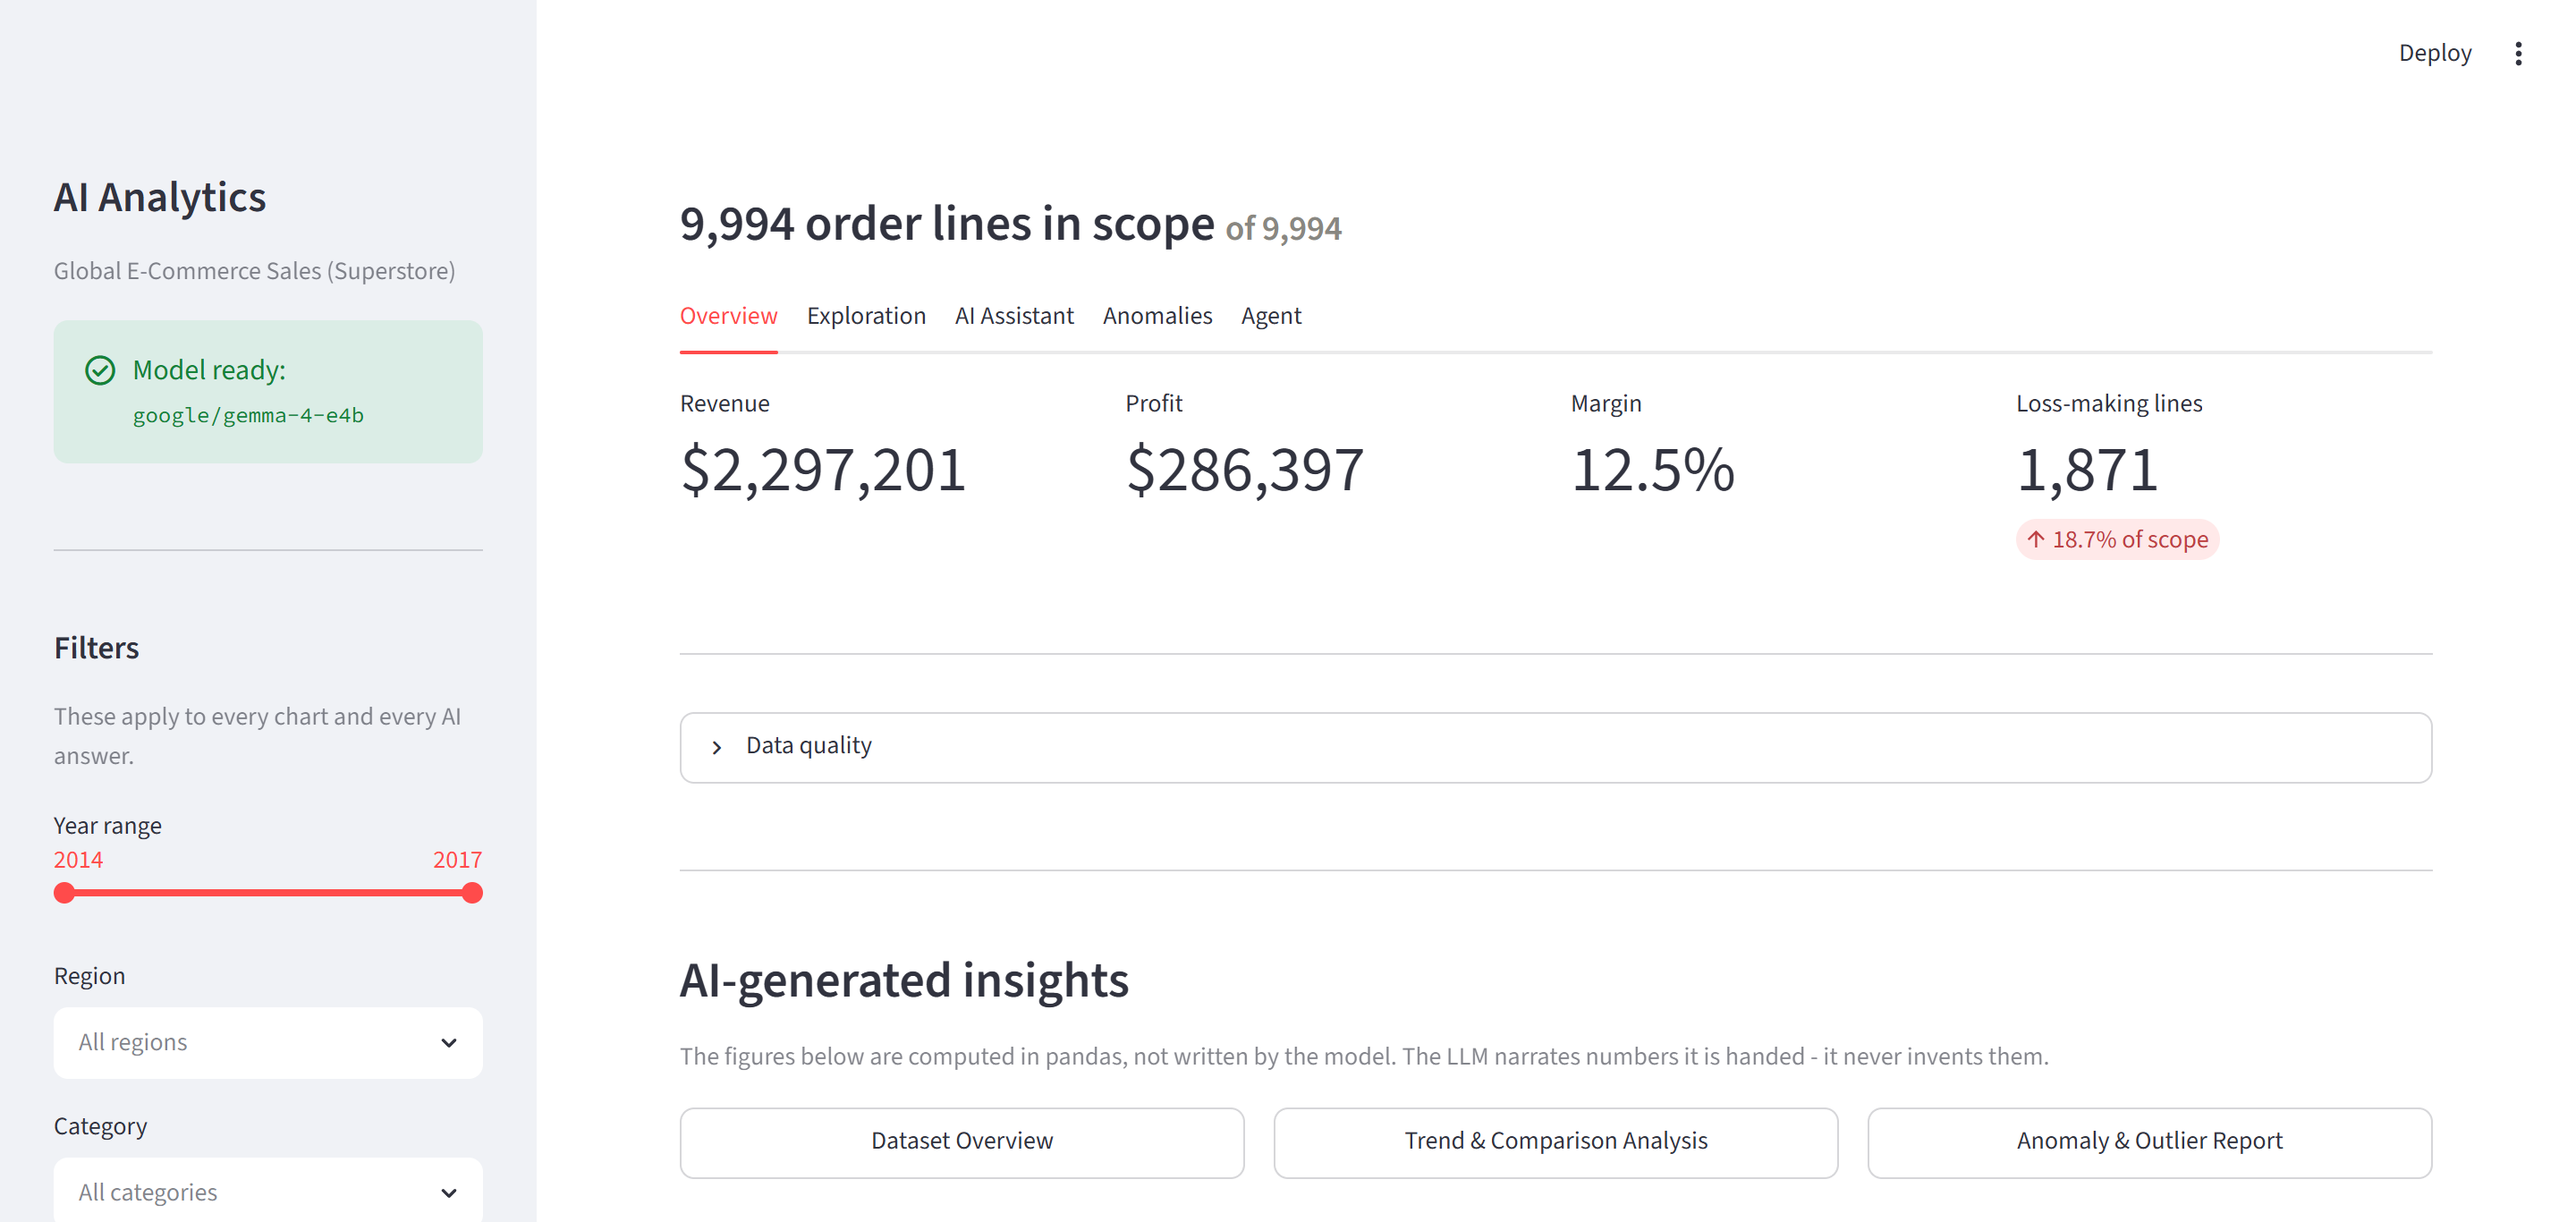
\includegraphics[width=\textwidth]{ui_overview.png}
  \caption{\textbf{Overview.} Totals, the data-quality card (A3) and the preset
  insights (B3). The sidebar filter panel is applied once and read by every tab.
  ``Model ready'' is a live health check, not a decoration: when the model is
  unreachable it turns red and says so.}
  \label{fig:ui-overview}
\end{minipage}\hfill
\begin{minipage}{0.49\textwidth}
  \centering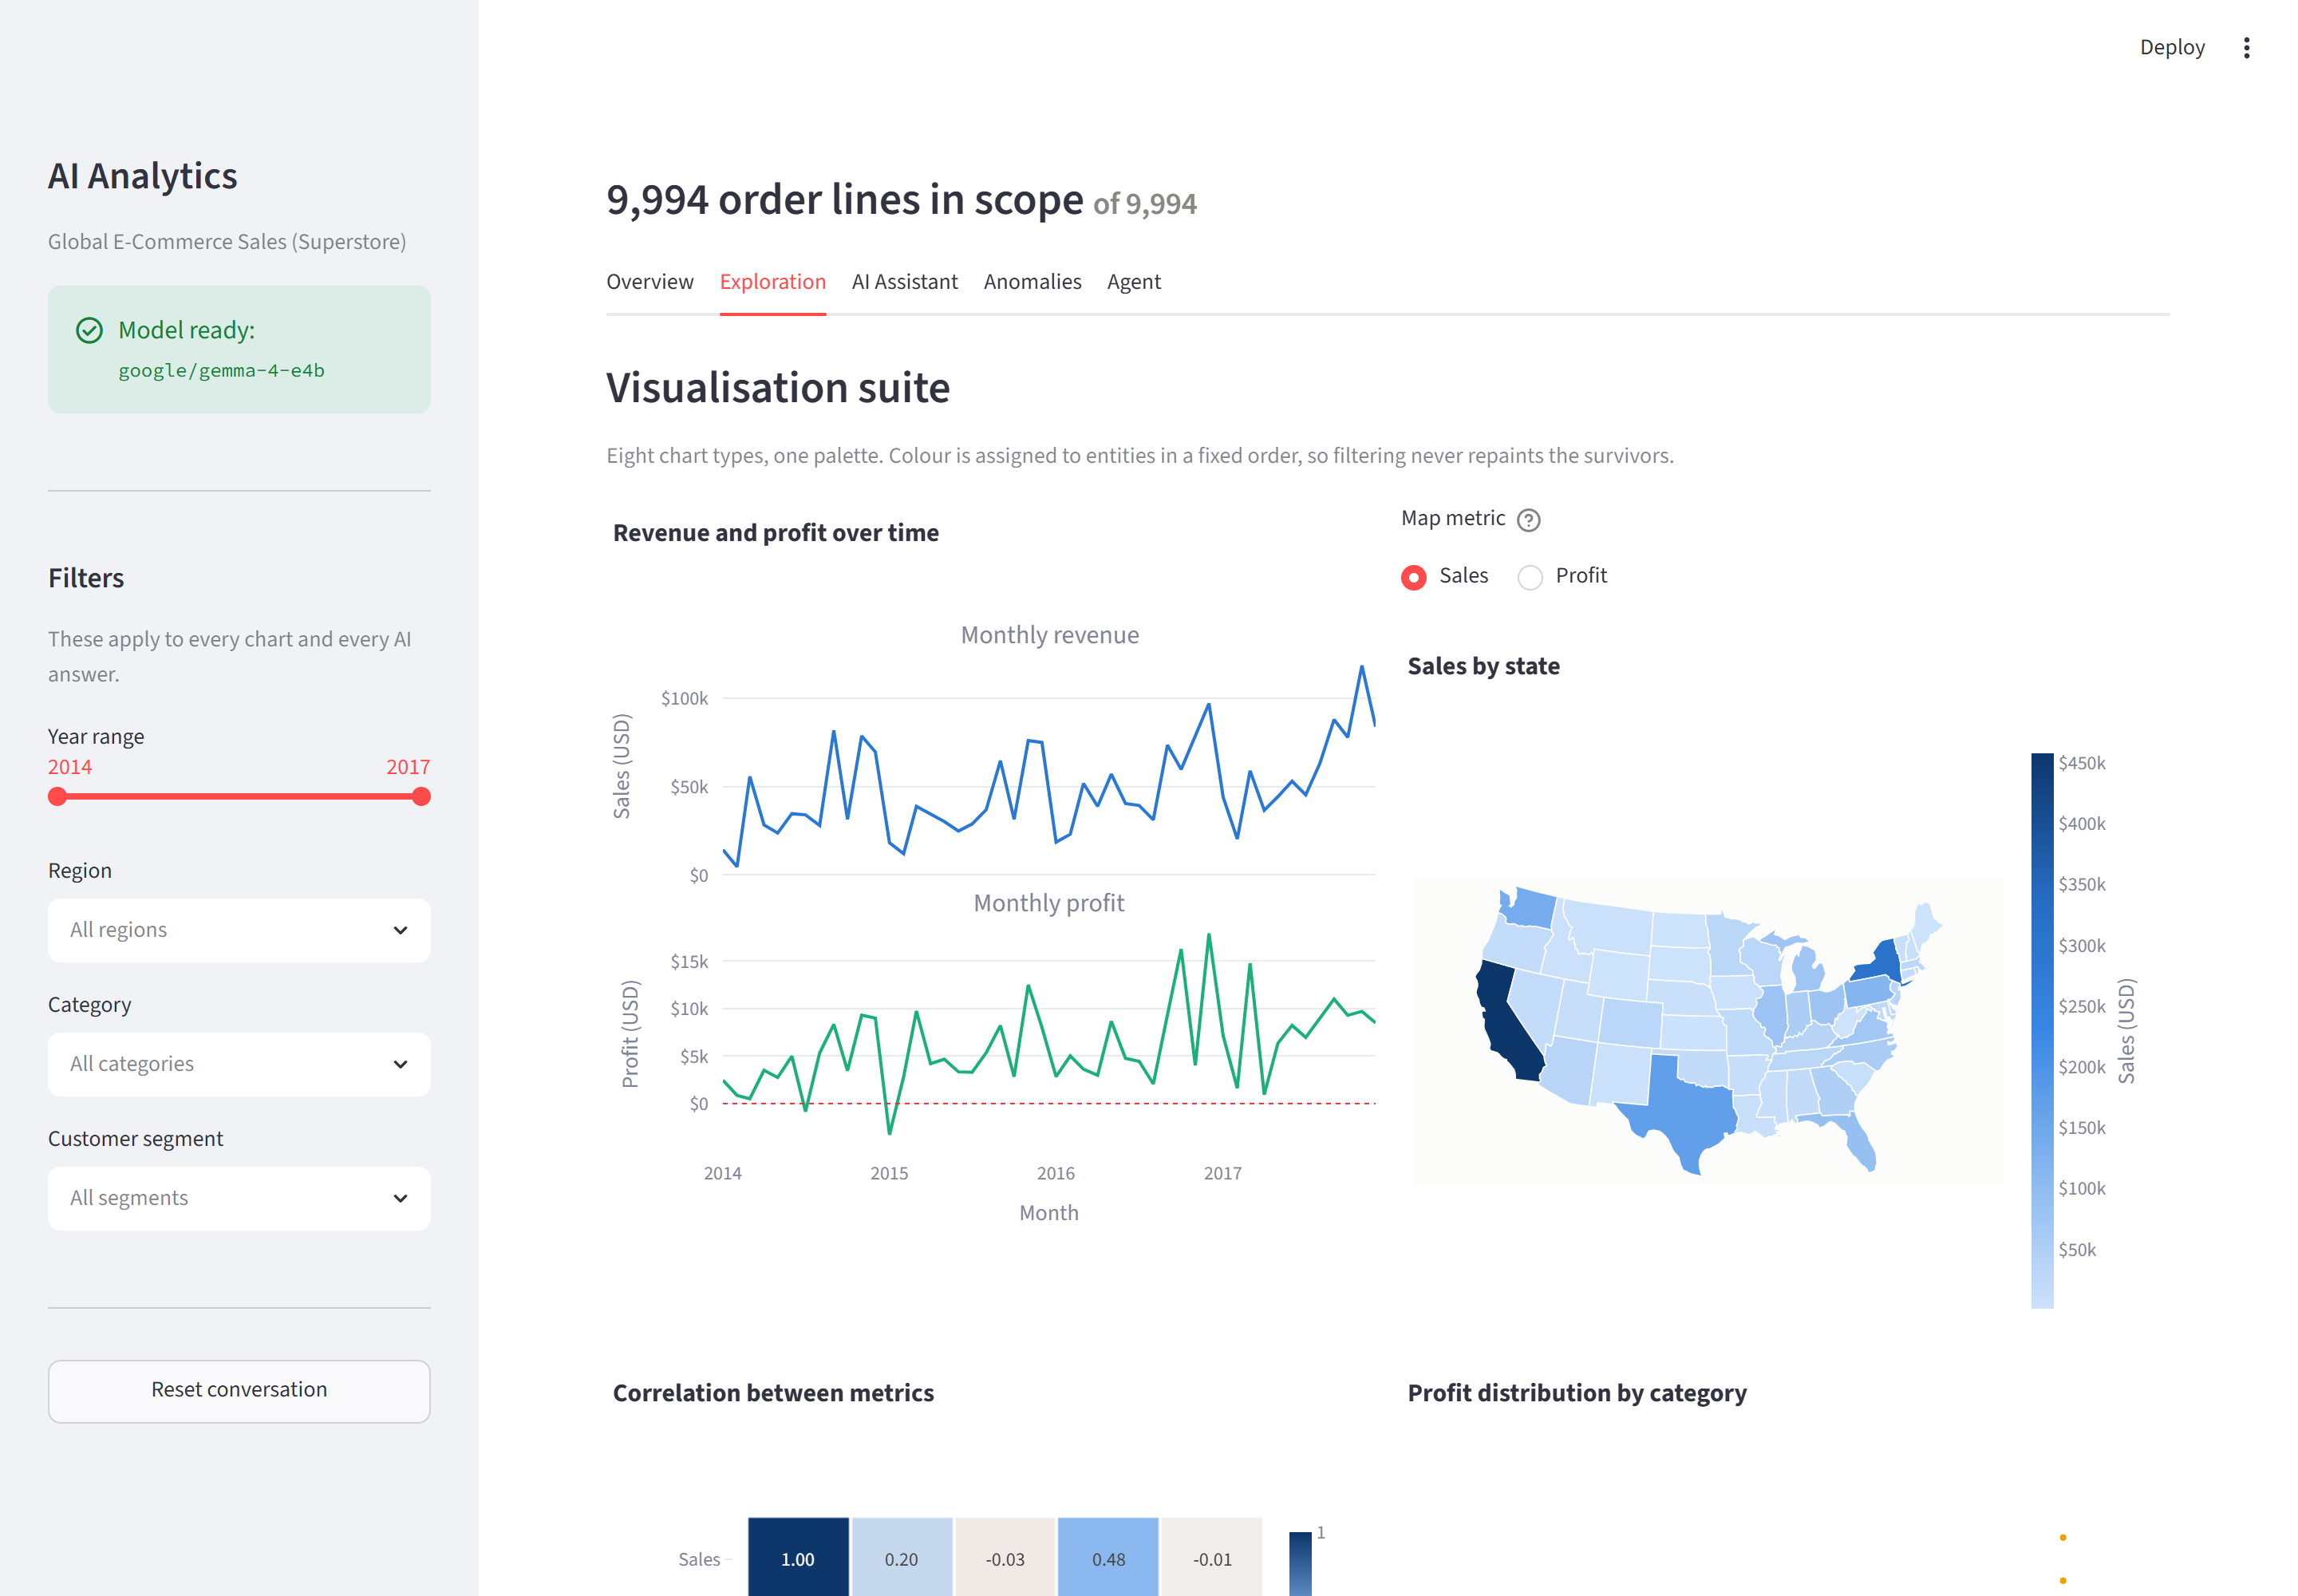
\includegraphics[width=\textwidth]{ui_exploration.png}
  \caption{\textbf{Exploration.} The chart suite (C2) over the filtered scope.
  Colour follows the entity, so changing a filter never repaints the survivors
  into different hues.}
  \label{fig:ui-exploration}
\end{minipage}
\end{figure}

\begin{figure}[htbp]
\centering
\begin{minipage}{0.49\textwidth}
  \centering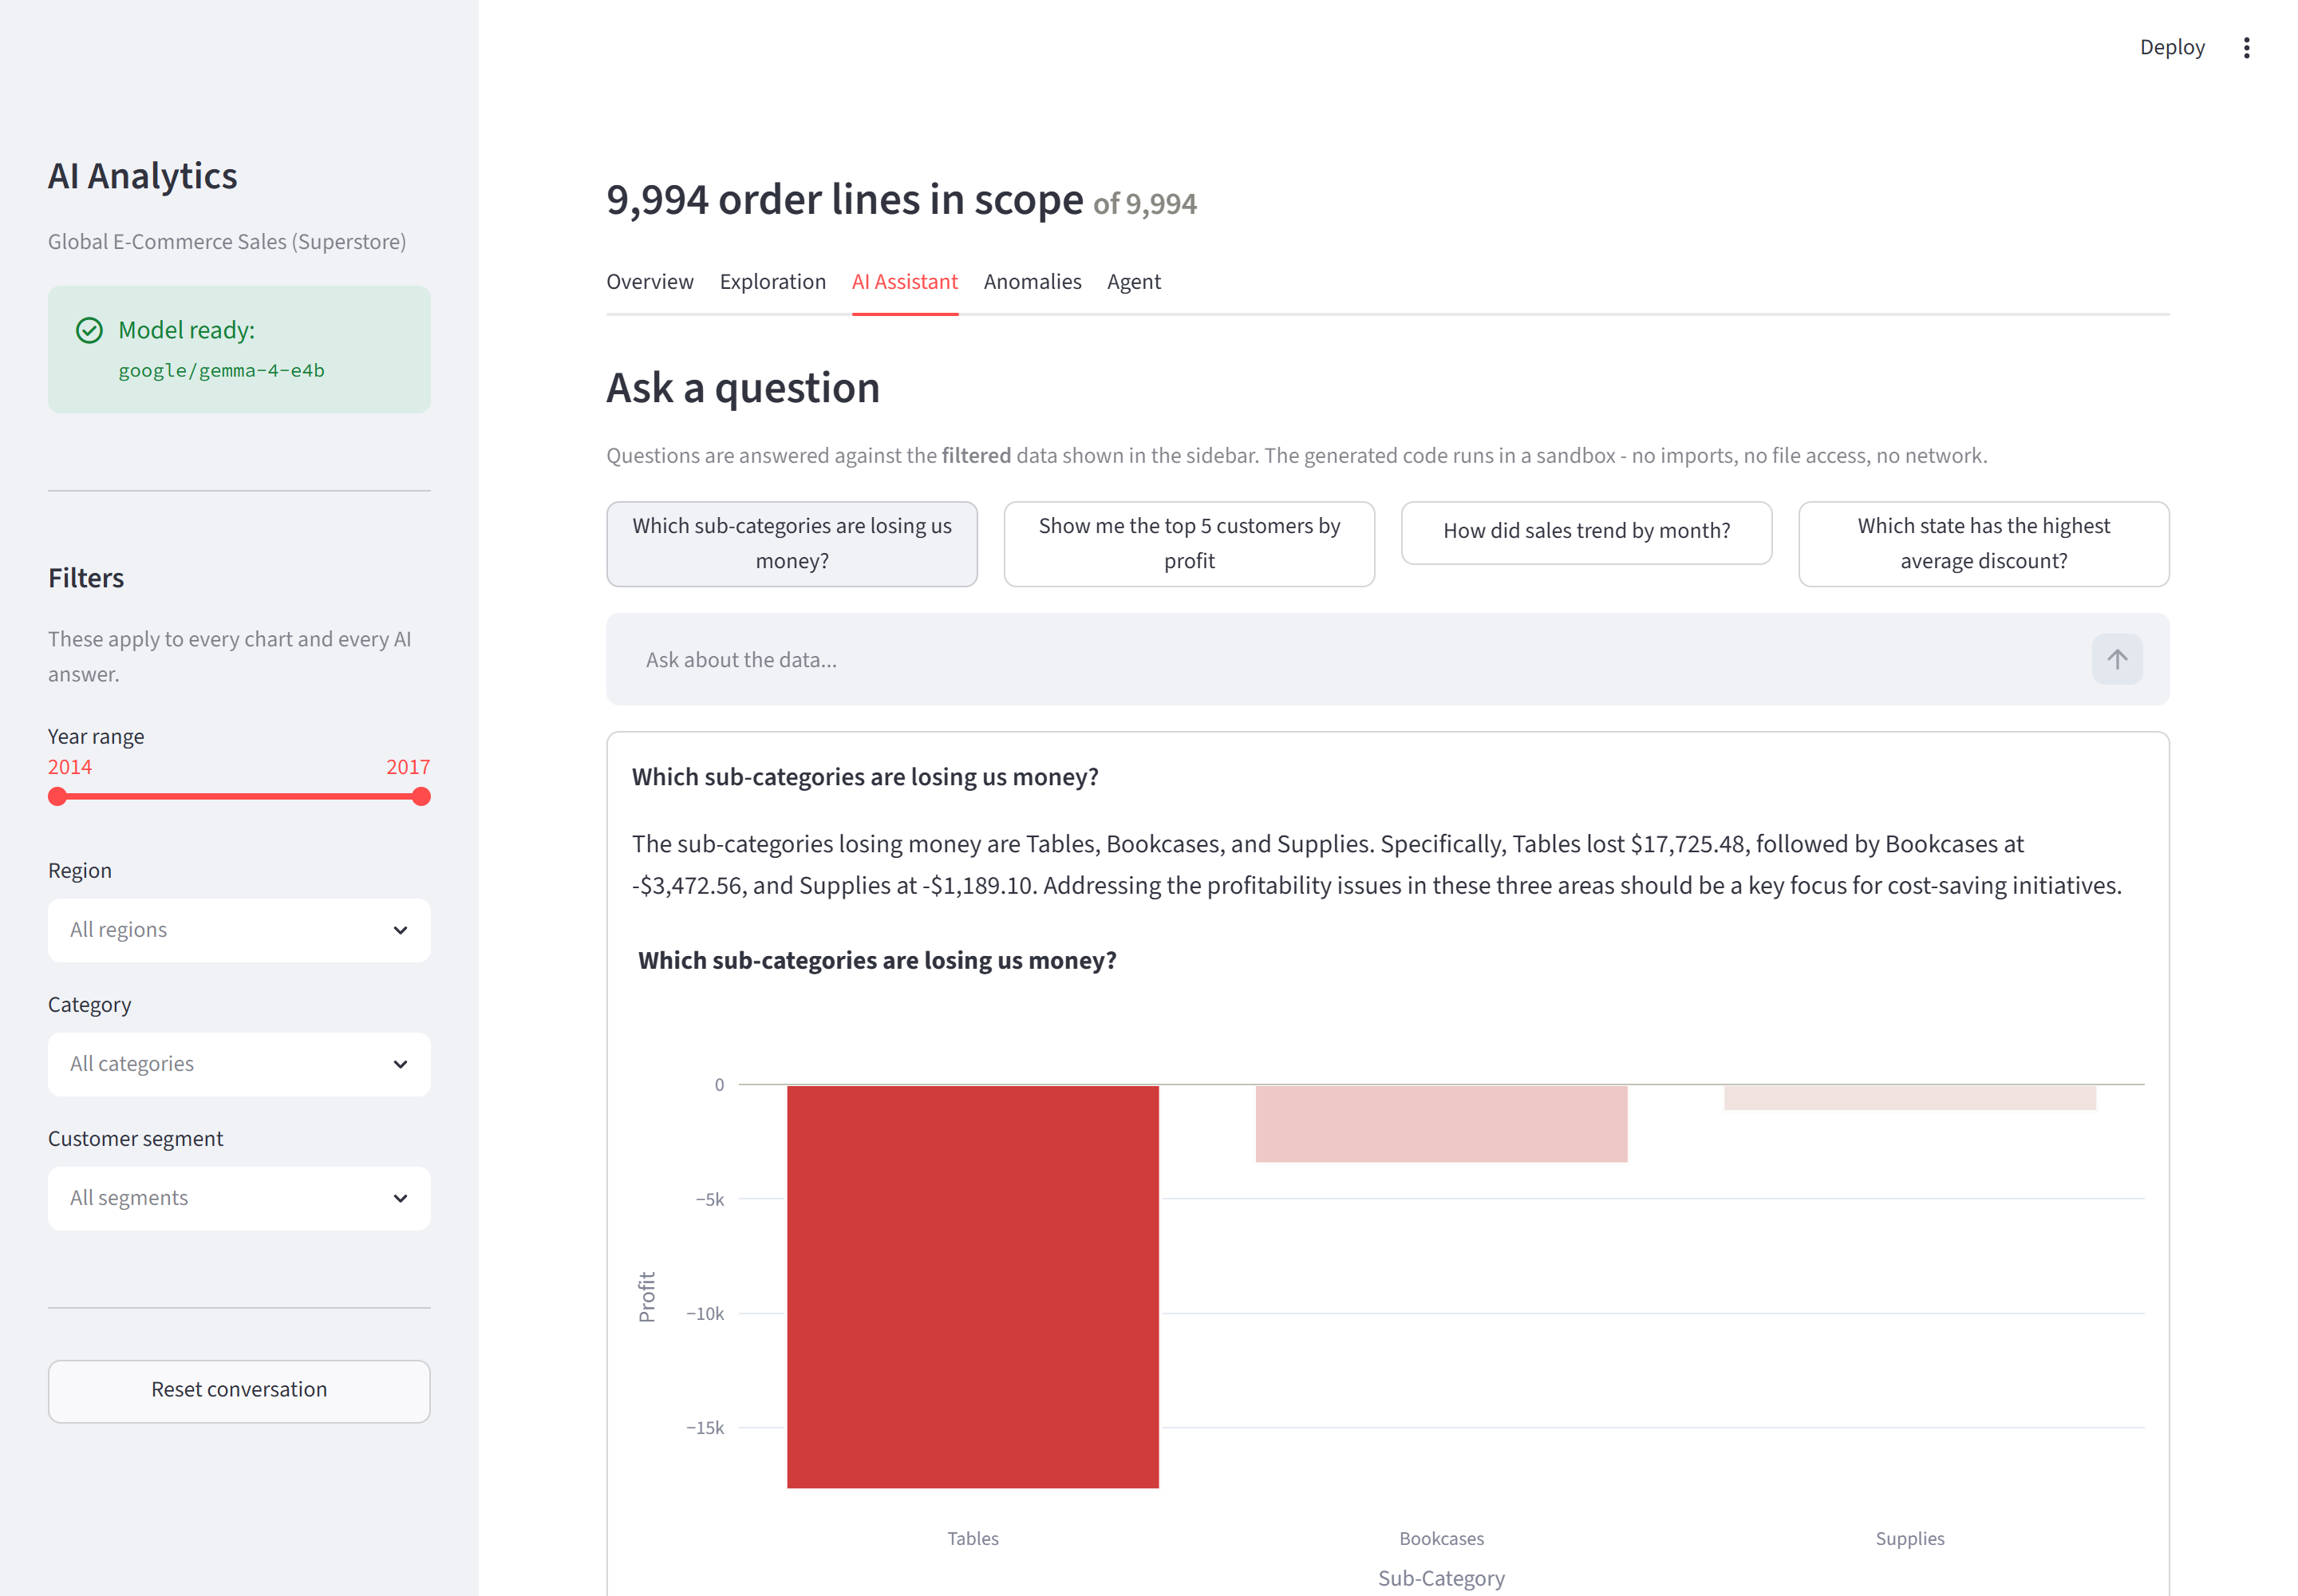
\includegraphics[width=\textwidth]{ui_ai_assistant.png}
  \caption{\textbf{AI Assistant.} A question answered end to end: Gemma wrote the
  pandas, the sandbox ran it, Gemma narrated the result, and \texttt{autochart}
  chose the bar chart from the result's shape and captioned it. The diverging
  scale is doing real work --- the losses are red because the metric is signed.}
  \label{fig:ui-ai}
\end{minipage}\hfill
\begin{minipage}{0.49\textwidth}
  \centering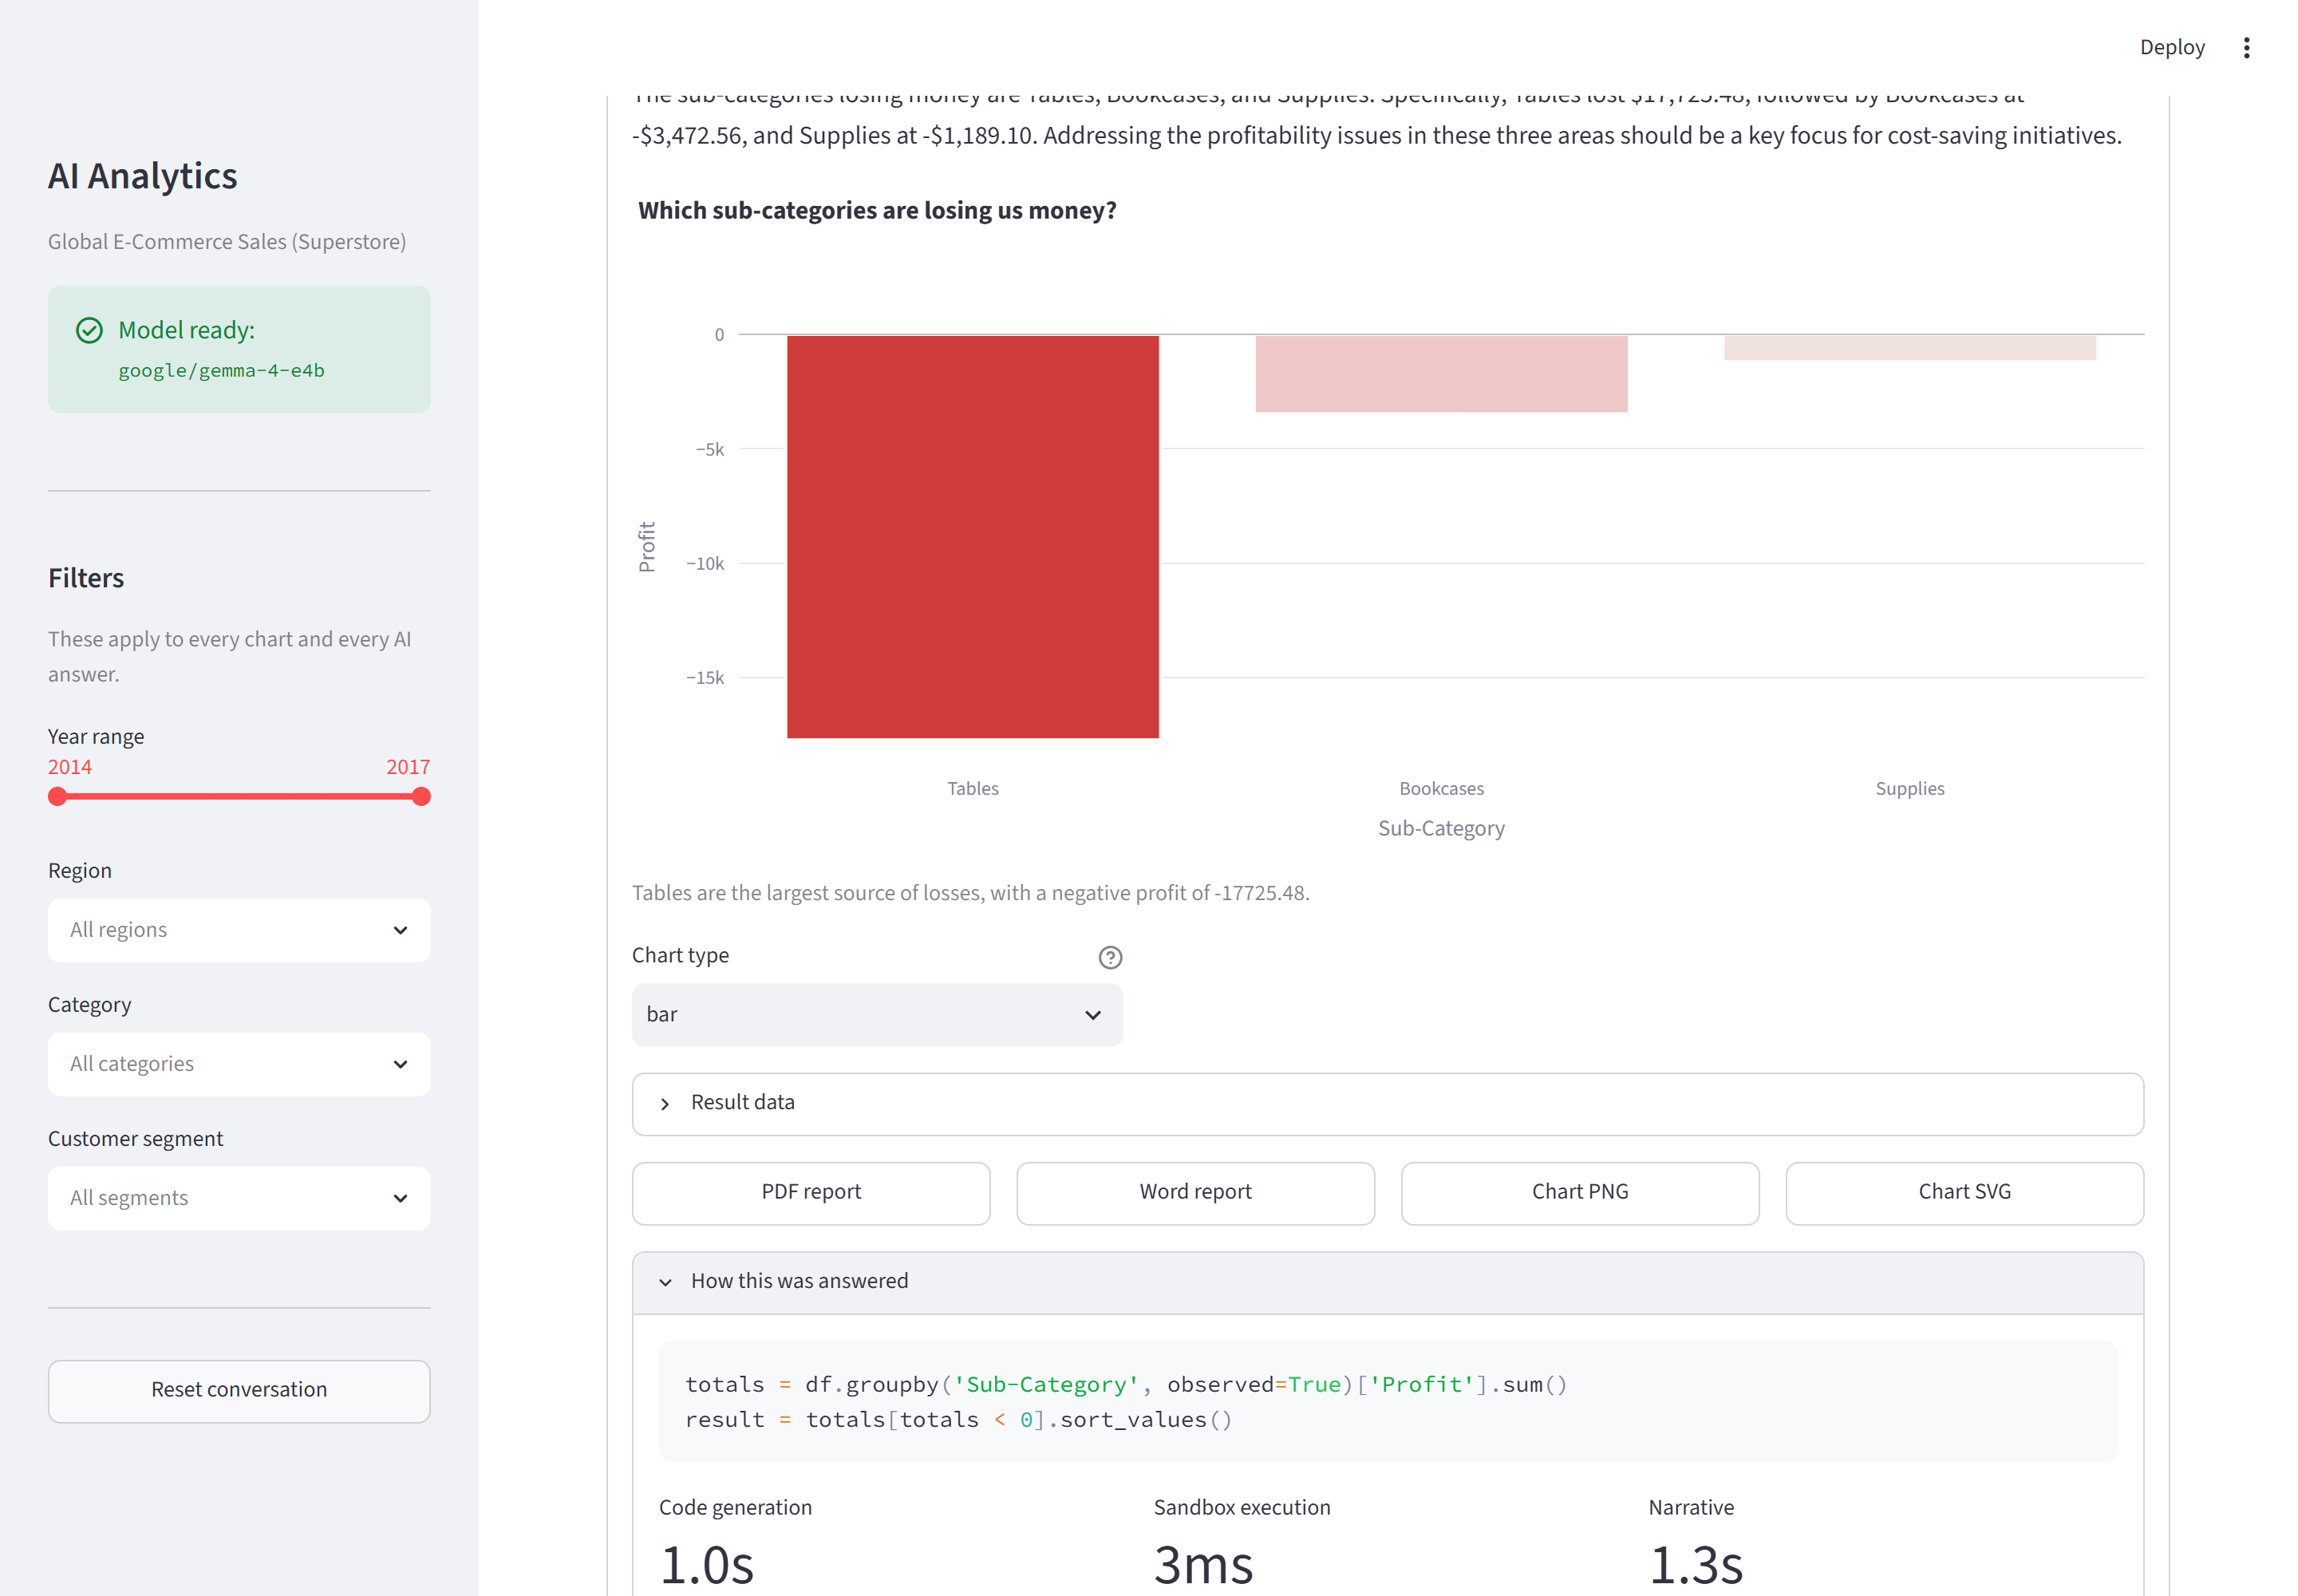
\includegraphics[width=\textwidth]{ui_ai_trace.png}
  \caption{\textbf{The same answer, opened up.} Every answer carries its evidence:
  the generated code and the phase timings. A reader who does not trust the number
  can read the query that produced it --- the whole argument for generating code
  rather than having the model recite figures.}
  \label{fig:ui-trace}
\end{minipage}
\end{figure}

\begin{figure}[htbp]
\centering
\begin{minipage}{0.49\textwidth}
  \centering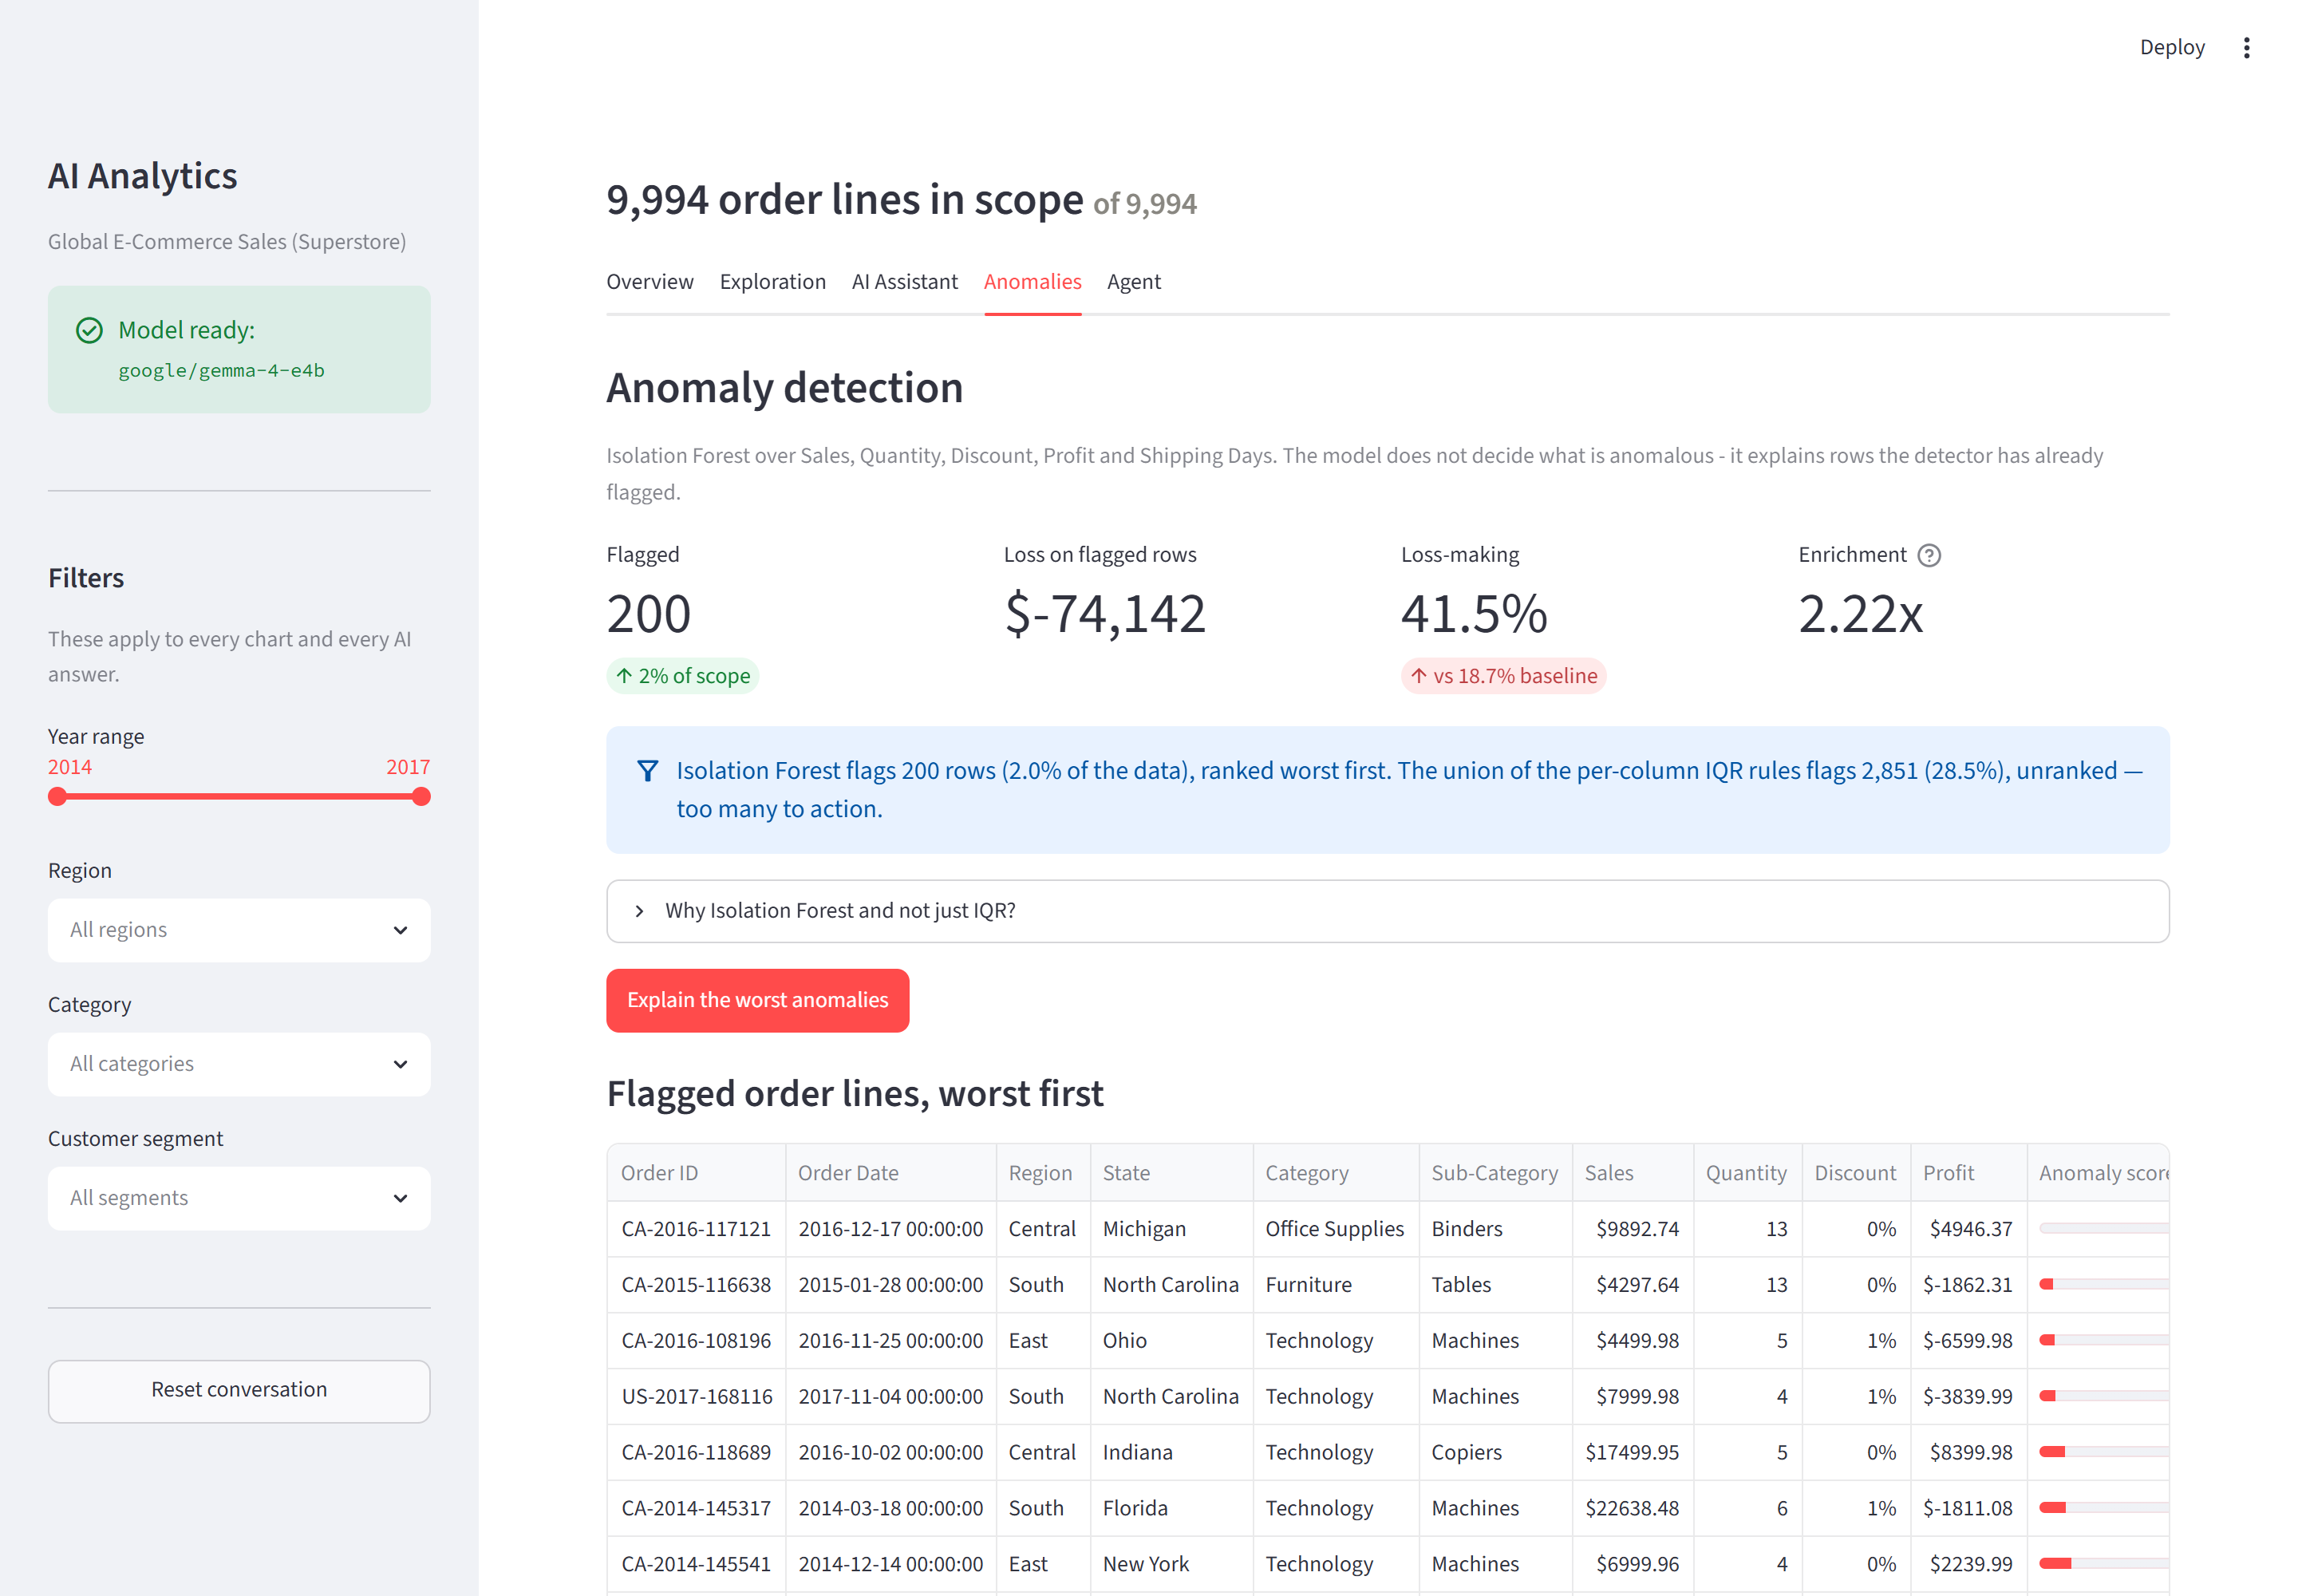
\includegraphics[width=\textwidth]{ui_anomalies.png}
  \caption{\textbf{Anomalies (D3).} The Isolation Forest's ranked output, worst
  first, with the LLM explaining rows the detector has already flagged. The model
  is never asked \emph{what} is anomalous.}
  \label{fig:ui-anomalies}
\end{minipage}\hfill
\begin{minipage}{0.49\textwidth}
  \centering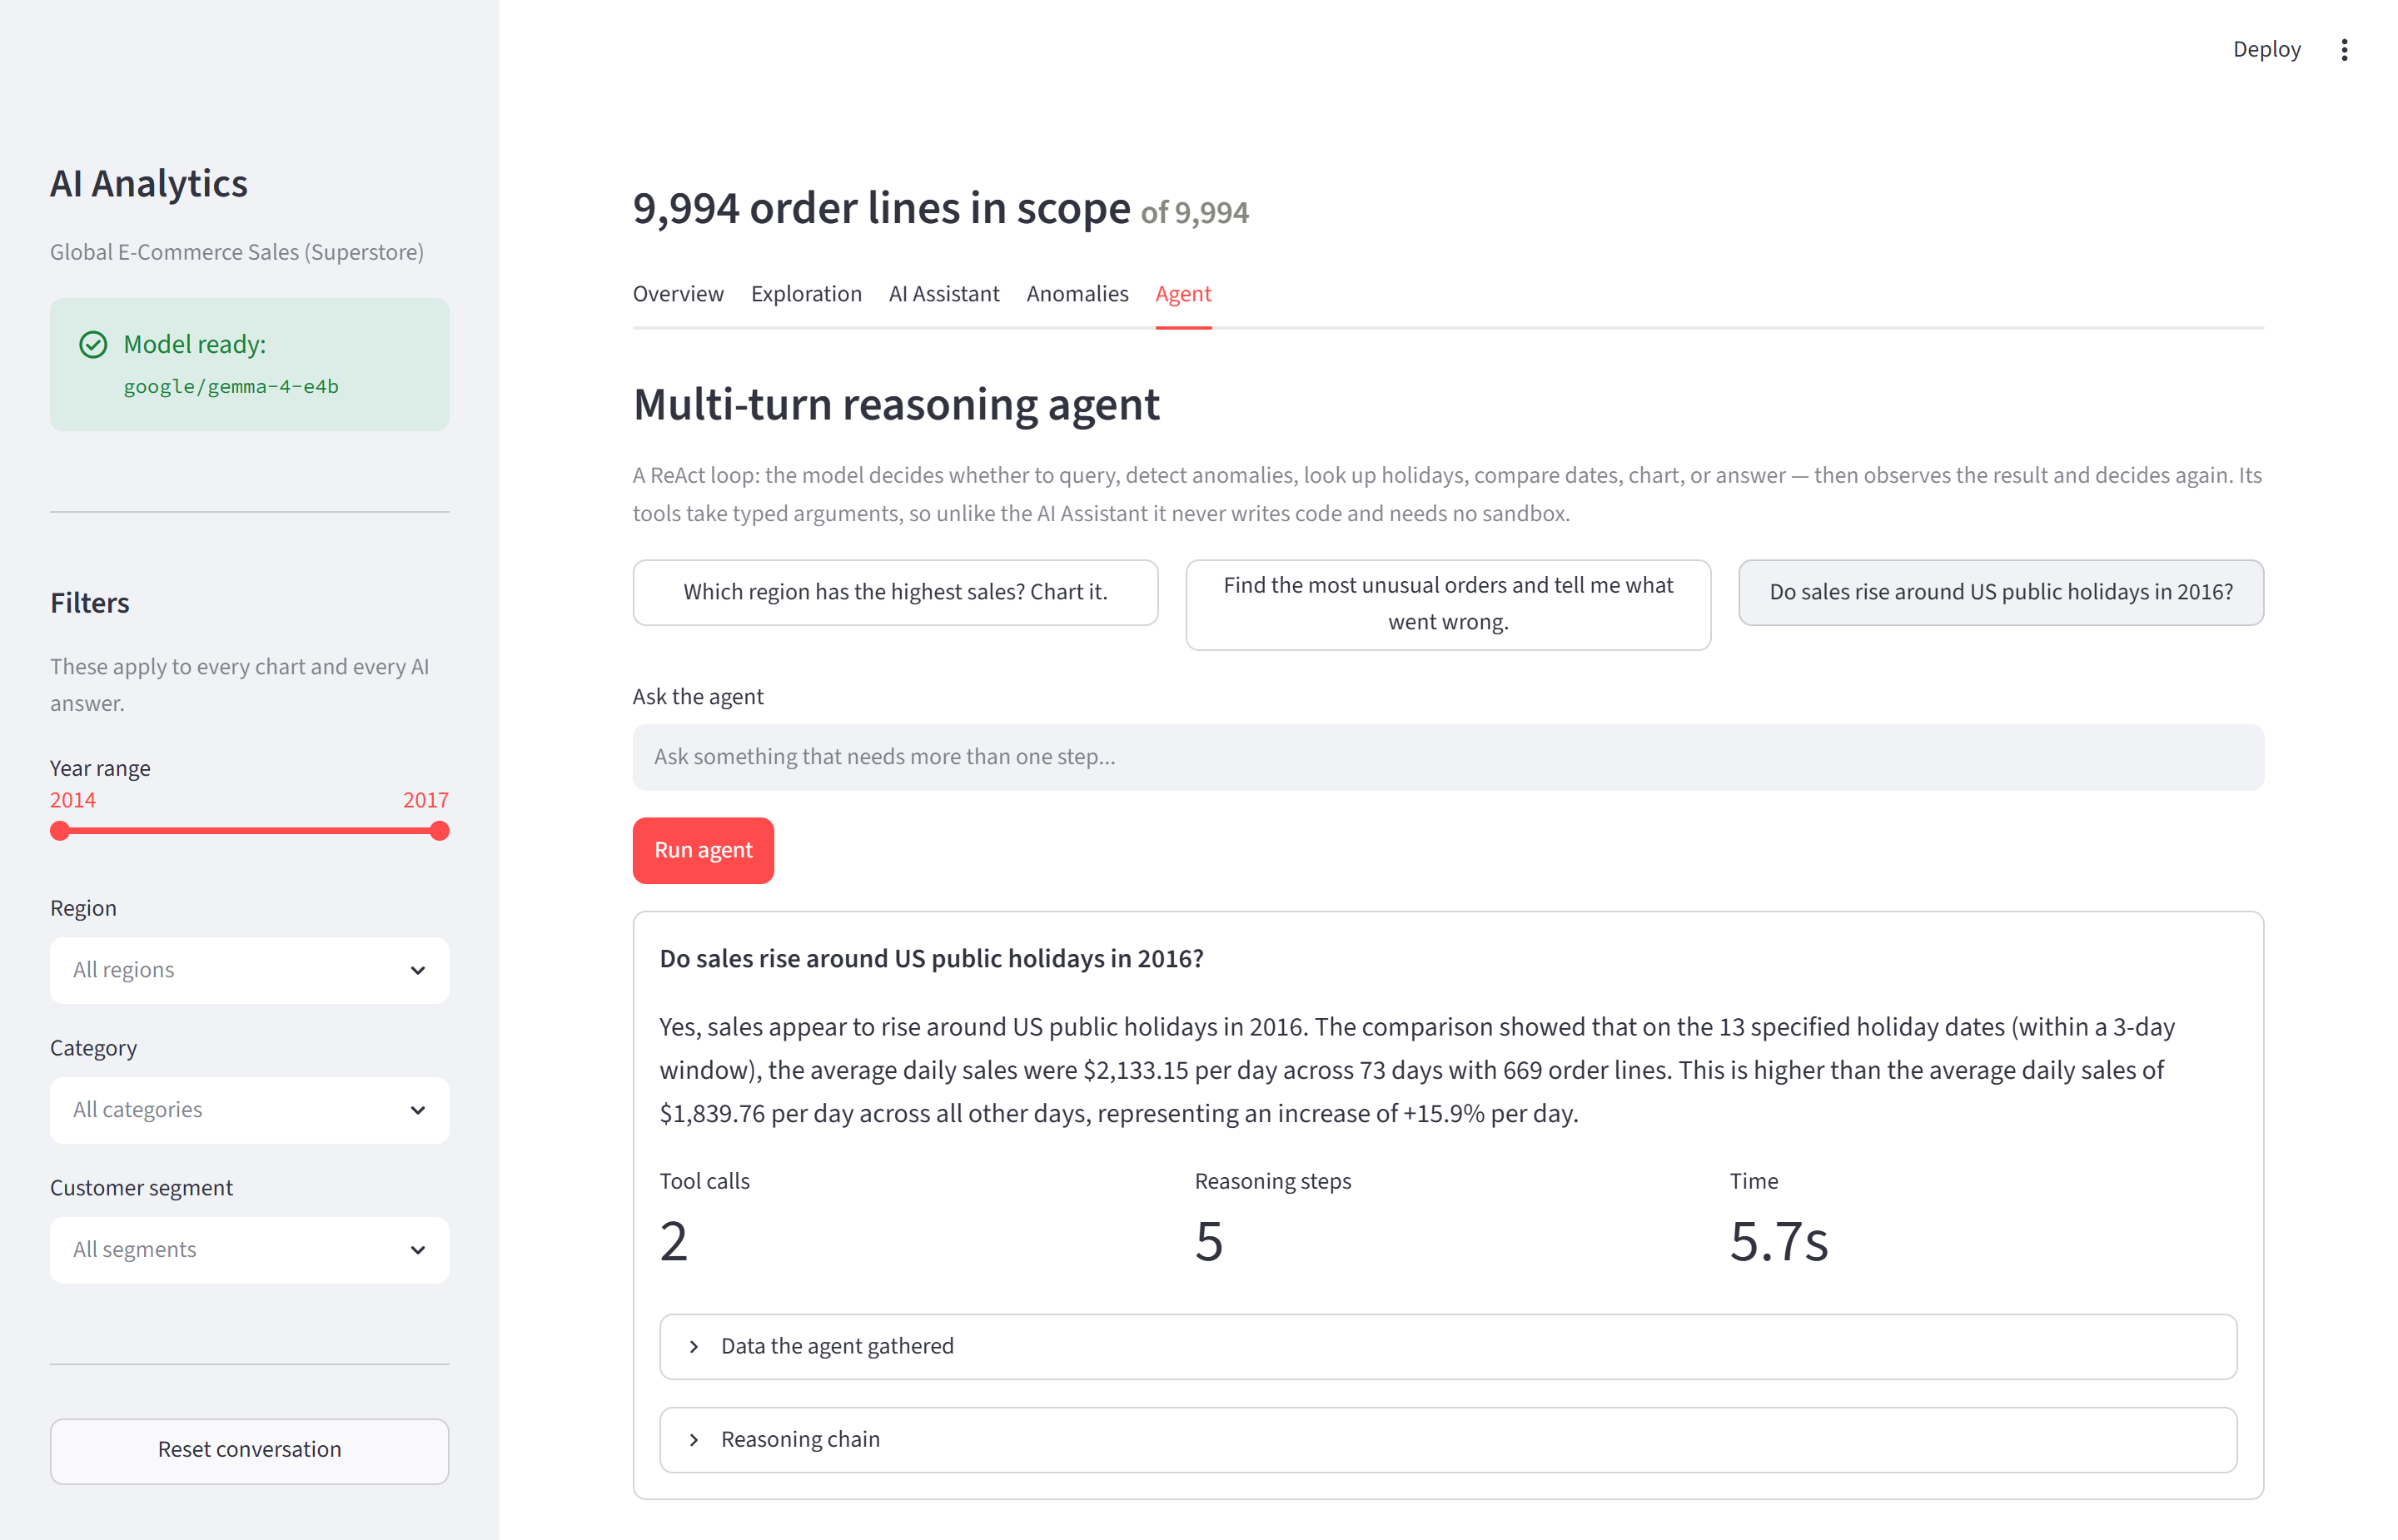
\includegraphics[width=\textwidth]{ui_agent.png}
  \caption{\textbf{Agent (D4).} The holiday question answered live: two tool calls
  in 6.0\,s, one of them to an external API, finding sales 15.9\% per day higher
  around US public holidays. Task B cannot answer this --- the fact is not in the
  dataset, and the second call's arguments are the first call's output.}
  \label{fig:ui-agent}
\end{minipage}
\end{figure}

\subsection{Colour system}

The palette was \textbf{validated with a colour-vision-deficiency checker, not chosen
by eye.}

\begin{center}
\begin{tabular}{@{}lll@{}}
\toprule
\textbf{Mode} & \textbf{Worst adjacent CVD separation} & \textbf{Contrast vs surface} \\
\midrule
Light & $\Delta E$ 24.2 (target $\ge$12) --- pass & 2 hues below 3:1 --- caution \\
Dark  & $\Delta E$ 10.3 (floor band) --- caution   & all $\ge$3:1 --- pass \\
\bottomrule
\end{tabular}
\end{center}

Both findings oblige the \textbf{same mitigation}, applied throughout: \textbf{colour is
never the only channel carrying identity.} Every multi-series chart ships a legend,
tooltips name the series, and a table view of the underlying data is available. A
red/green-colourblind viewer can read every chart in this application.

Three encodings, three colour jobs:

\begin{itemize}[leftmargin=*]
\item \textbf{Categorical $\rightarrow$ identity.} Eight fixed slots, assigned in sorted
      order and \textbf{never cycled}. Colour follows the \emph{entity}, not its rank:
      filtering out a region never repaints the survivors.
\item \textbf{Sequential $\rightarrow$ magnitude.} One blue hue, light$\rightarrow$dark.
      Used for Sales.
\item \textbf{Diverging $\rightarrow$ polarity.} Blue$\leftrightarrow$red with a
      \textbf{neutral grey midpoint}. Used for Profit, because the \emph{sign} is the
      point: a state losing money must not look like a state making a little.
\end{itemize}

A rainbow scale is used nowhere. It implies an ordering the data does not have and is
unreadable under CVD.

\subsection{The chart suite}

Eight chart types against a required six.

\begin{center}
\begin{tabularx}{\textwidth}{@{}clX@{}}
\toprule
\textbf{\#} & \textbf{Chart} & \textbf{Design decision} \\
\midrule
1 & Revenue \& profit trend      & \textbf{Small multiples, NOT dual-axis} --- see \S\ref{sec:dual} \\
2 & State choropleth             & Sequential for Sales; \textbf{diverging for Profit}, anchored symmetrically on zero \\
3 & Correlation matrix           & Diverging, anchored at 0: $-1$ must look as strong as $+1$ \\
4 & Profit distribution          & \textbf{Box plot, not histogram} --- the question is spread and the long negative tail; a histogram of a skewed variable hides exactly that \\
5 & Category sunburst            & The hierarchy is \emph{genuine} (each sub-category has exactly one parent) --- the precondition for an honest sunburst rather than a decorative one \\
6 & Animated year-over-year      & \textbf{Y-axis fixed across frames.} Per-frame rescaling would make every year look identical and destroy the comparison the animation exists to make \\
7 & Discount vs profit scatter   & Least-squares fit + \textbf{95\% CI on the mean response}, computed explicitly rather than left to library defaults \\
8 & Segment $\times$ category    & Stacked bar, 2px surface gap between fills \\
\bottomrule
\end{tabularx}
\end{center}

\begin{figure}[htbp]
\centering
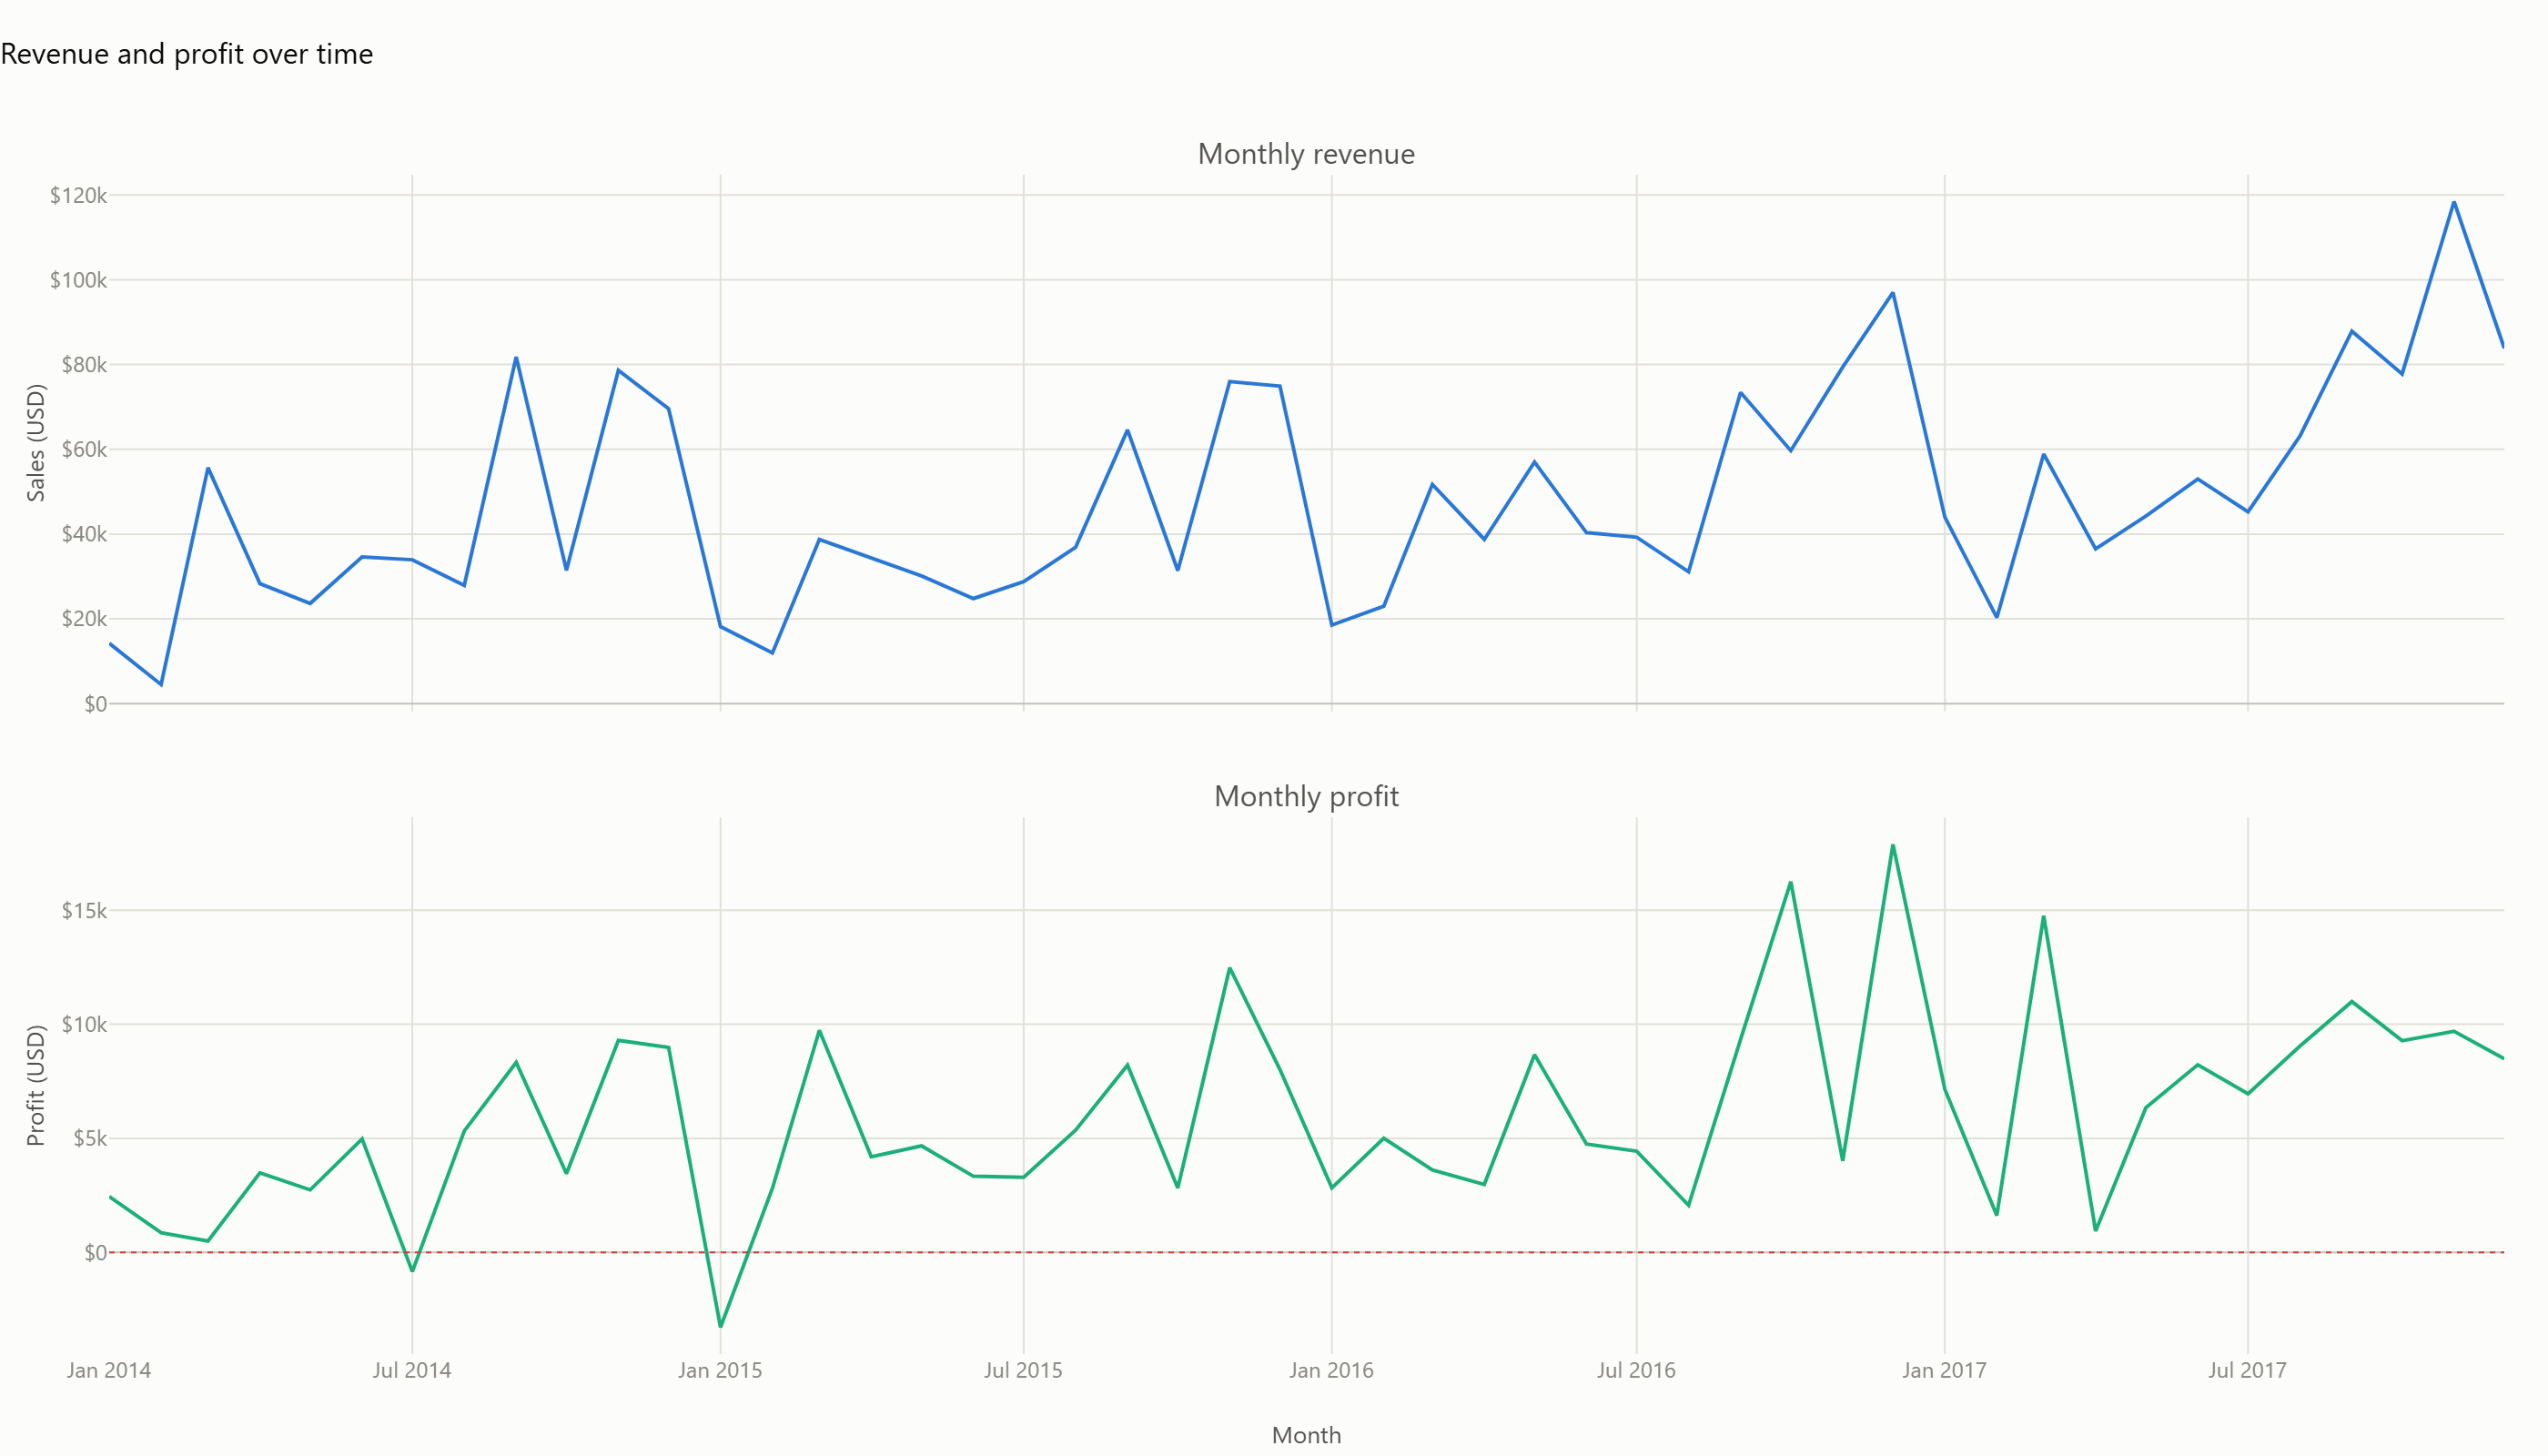
\includegraphics[width=0.66\textwidth]{trend_light.png}
\caption{Revenue and profit trend as small multiples. Shared x-axis, independent
truthful y-scales --- the honest alternative to a dual axis (\S\ref{sec:dual}).}
\end{figure}

\begin{figure}[htbp]
\centering
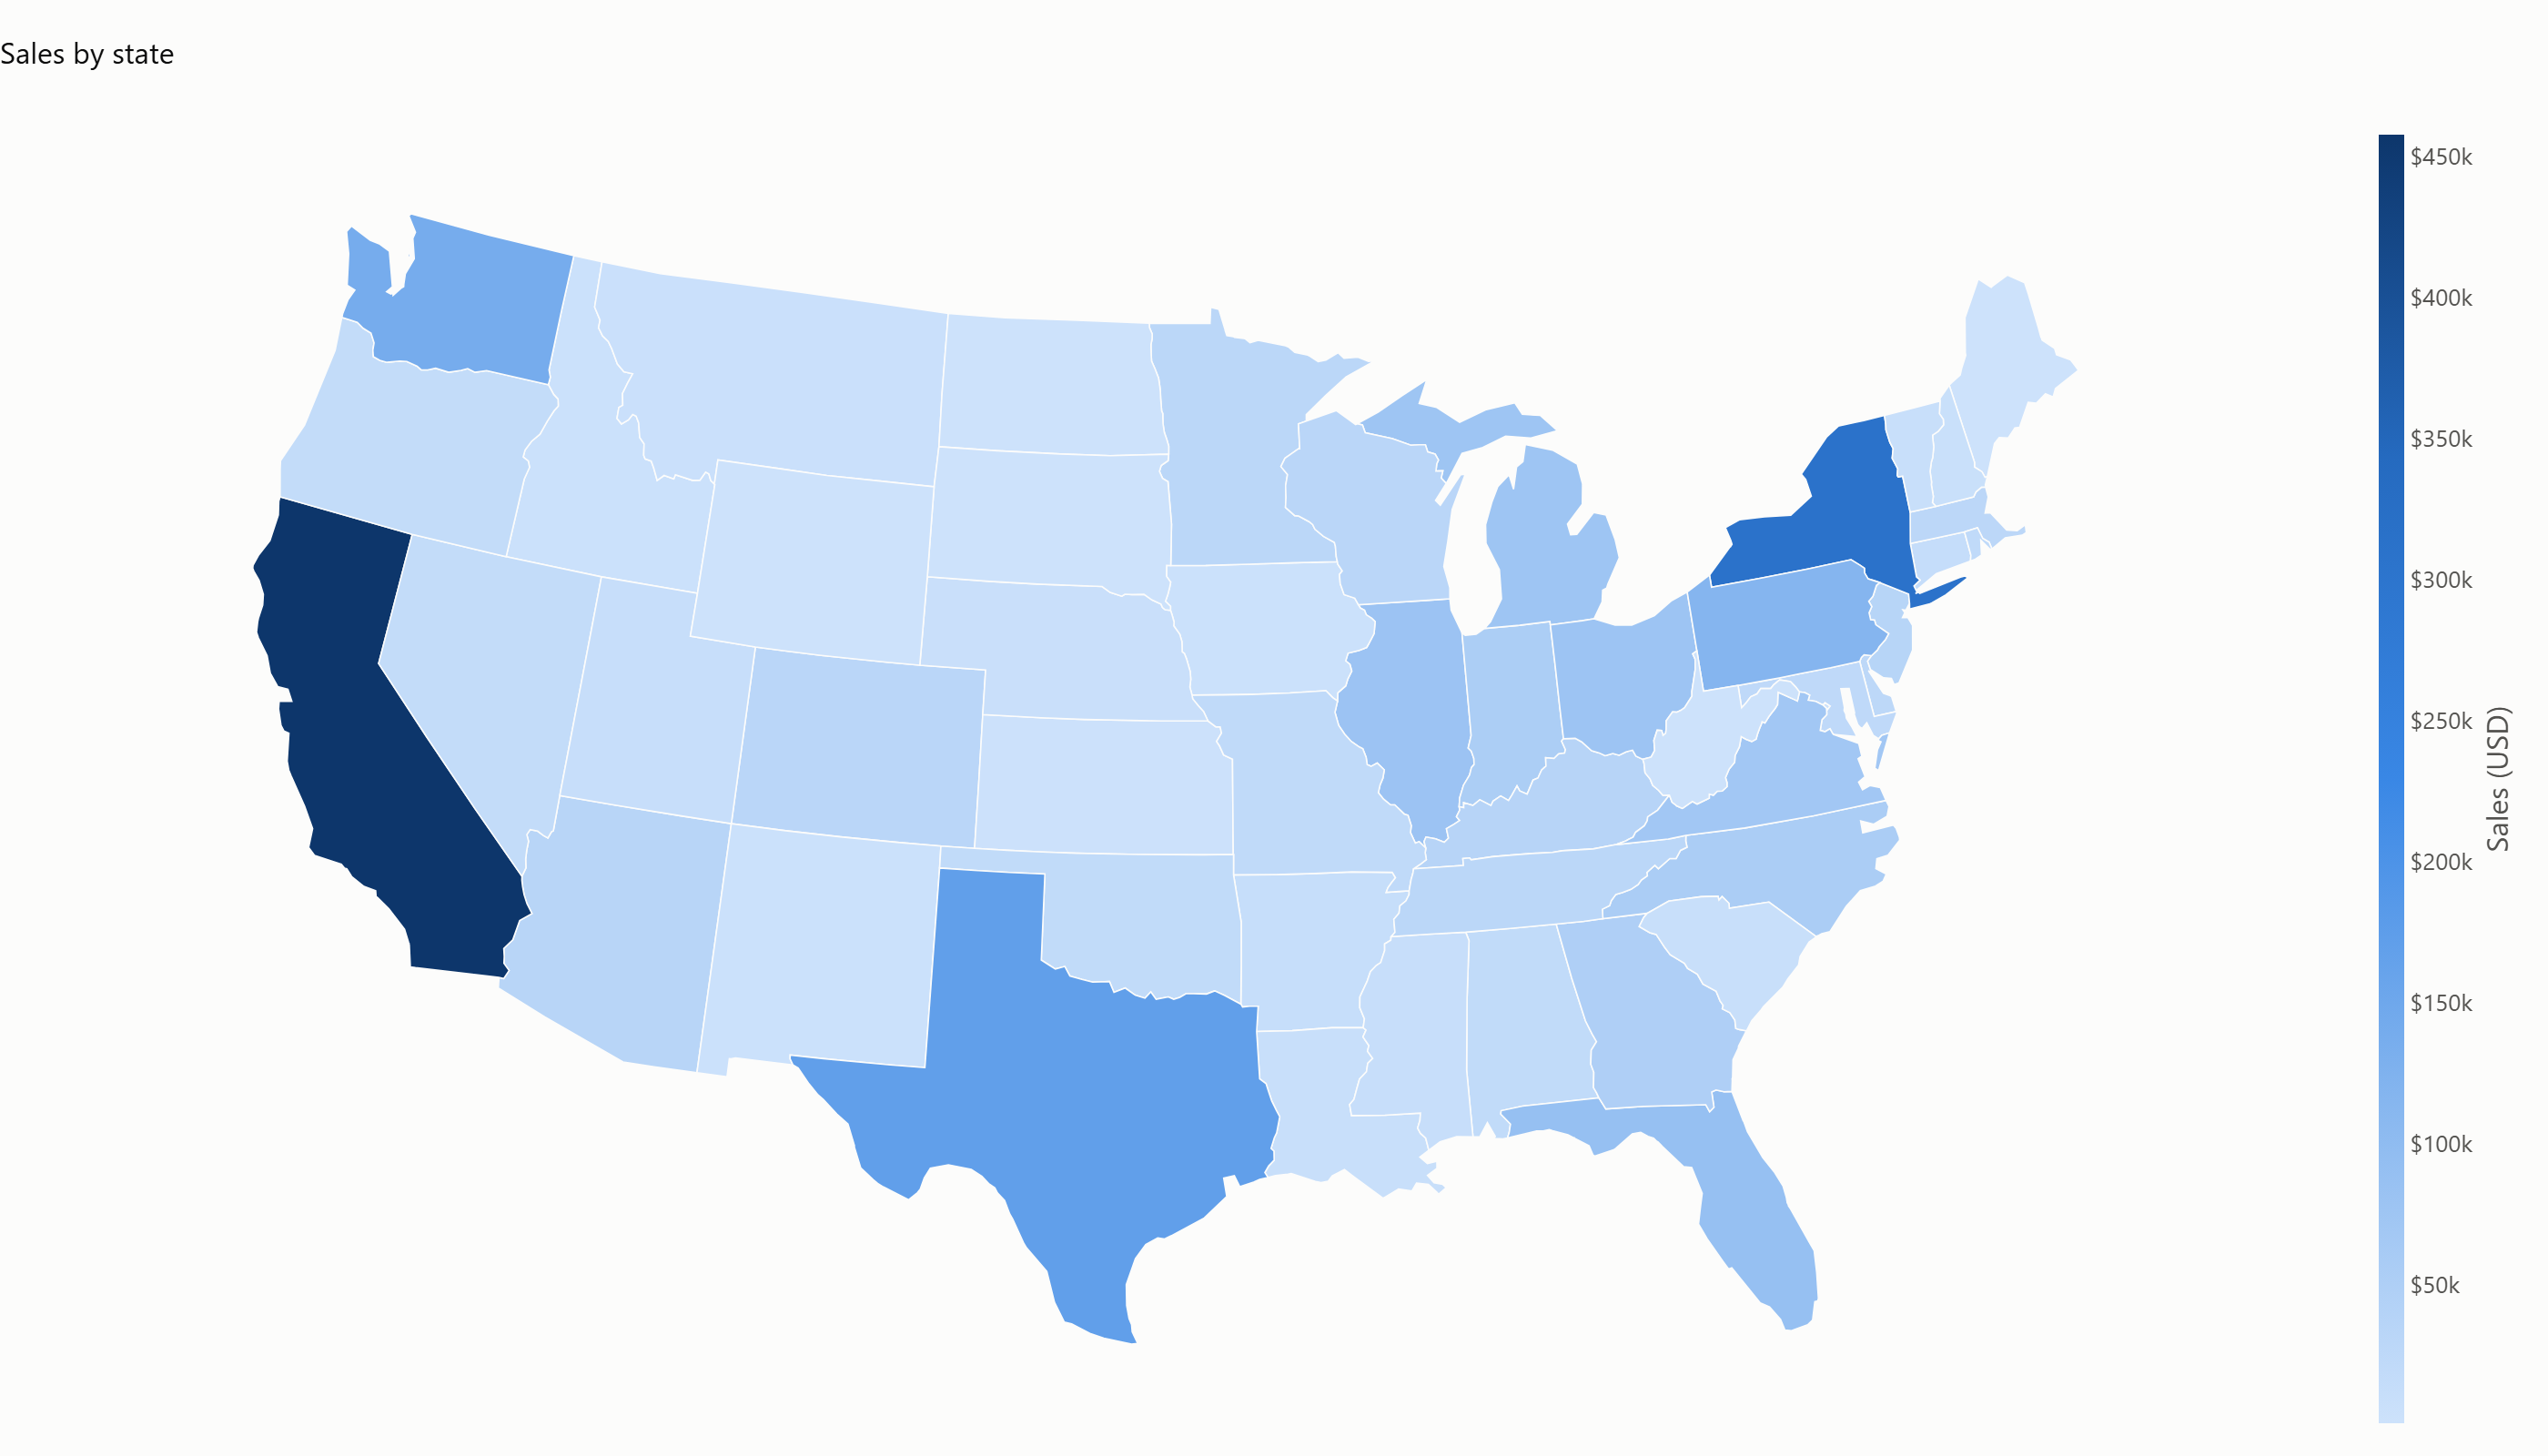
\includegraphics[width=0.60\textwidth]{map_light.png}
\caption{Sales by state: sequential single-hue blue, because sales is a magnitude
and more is simply more. Switching the metric to Profit in the app switches the
scale to diverging blue/red with a neutral grey midpoint, so that a loss-making
state cannot read as a state making a little.}
\end{figure}

\begin{figure}[htbp]
\centering
\begin{minipage}{0.49\textwidth}
  \centering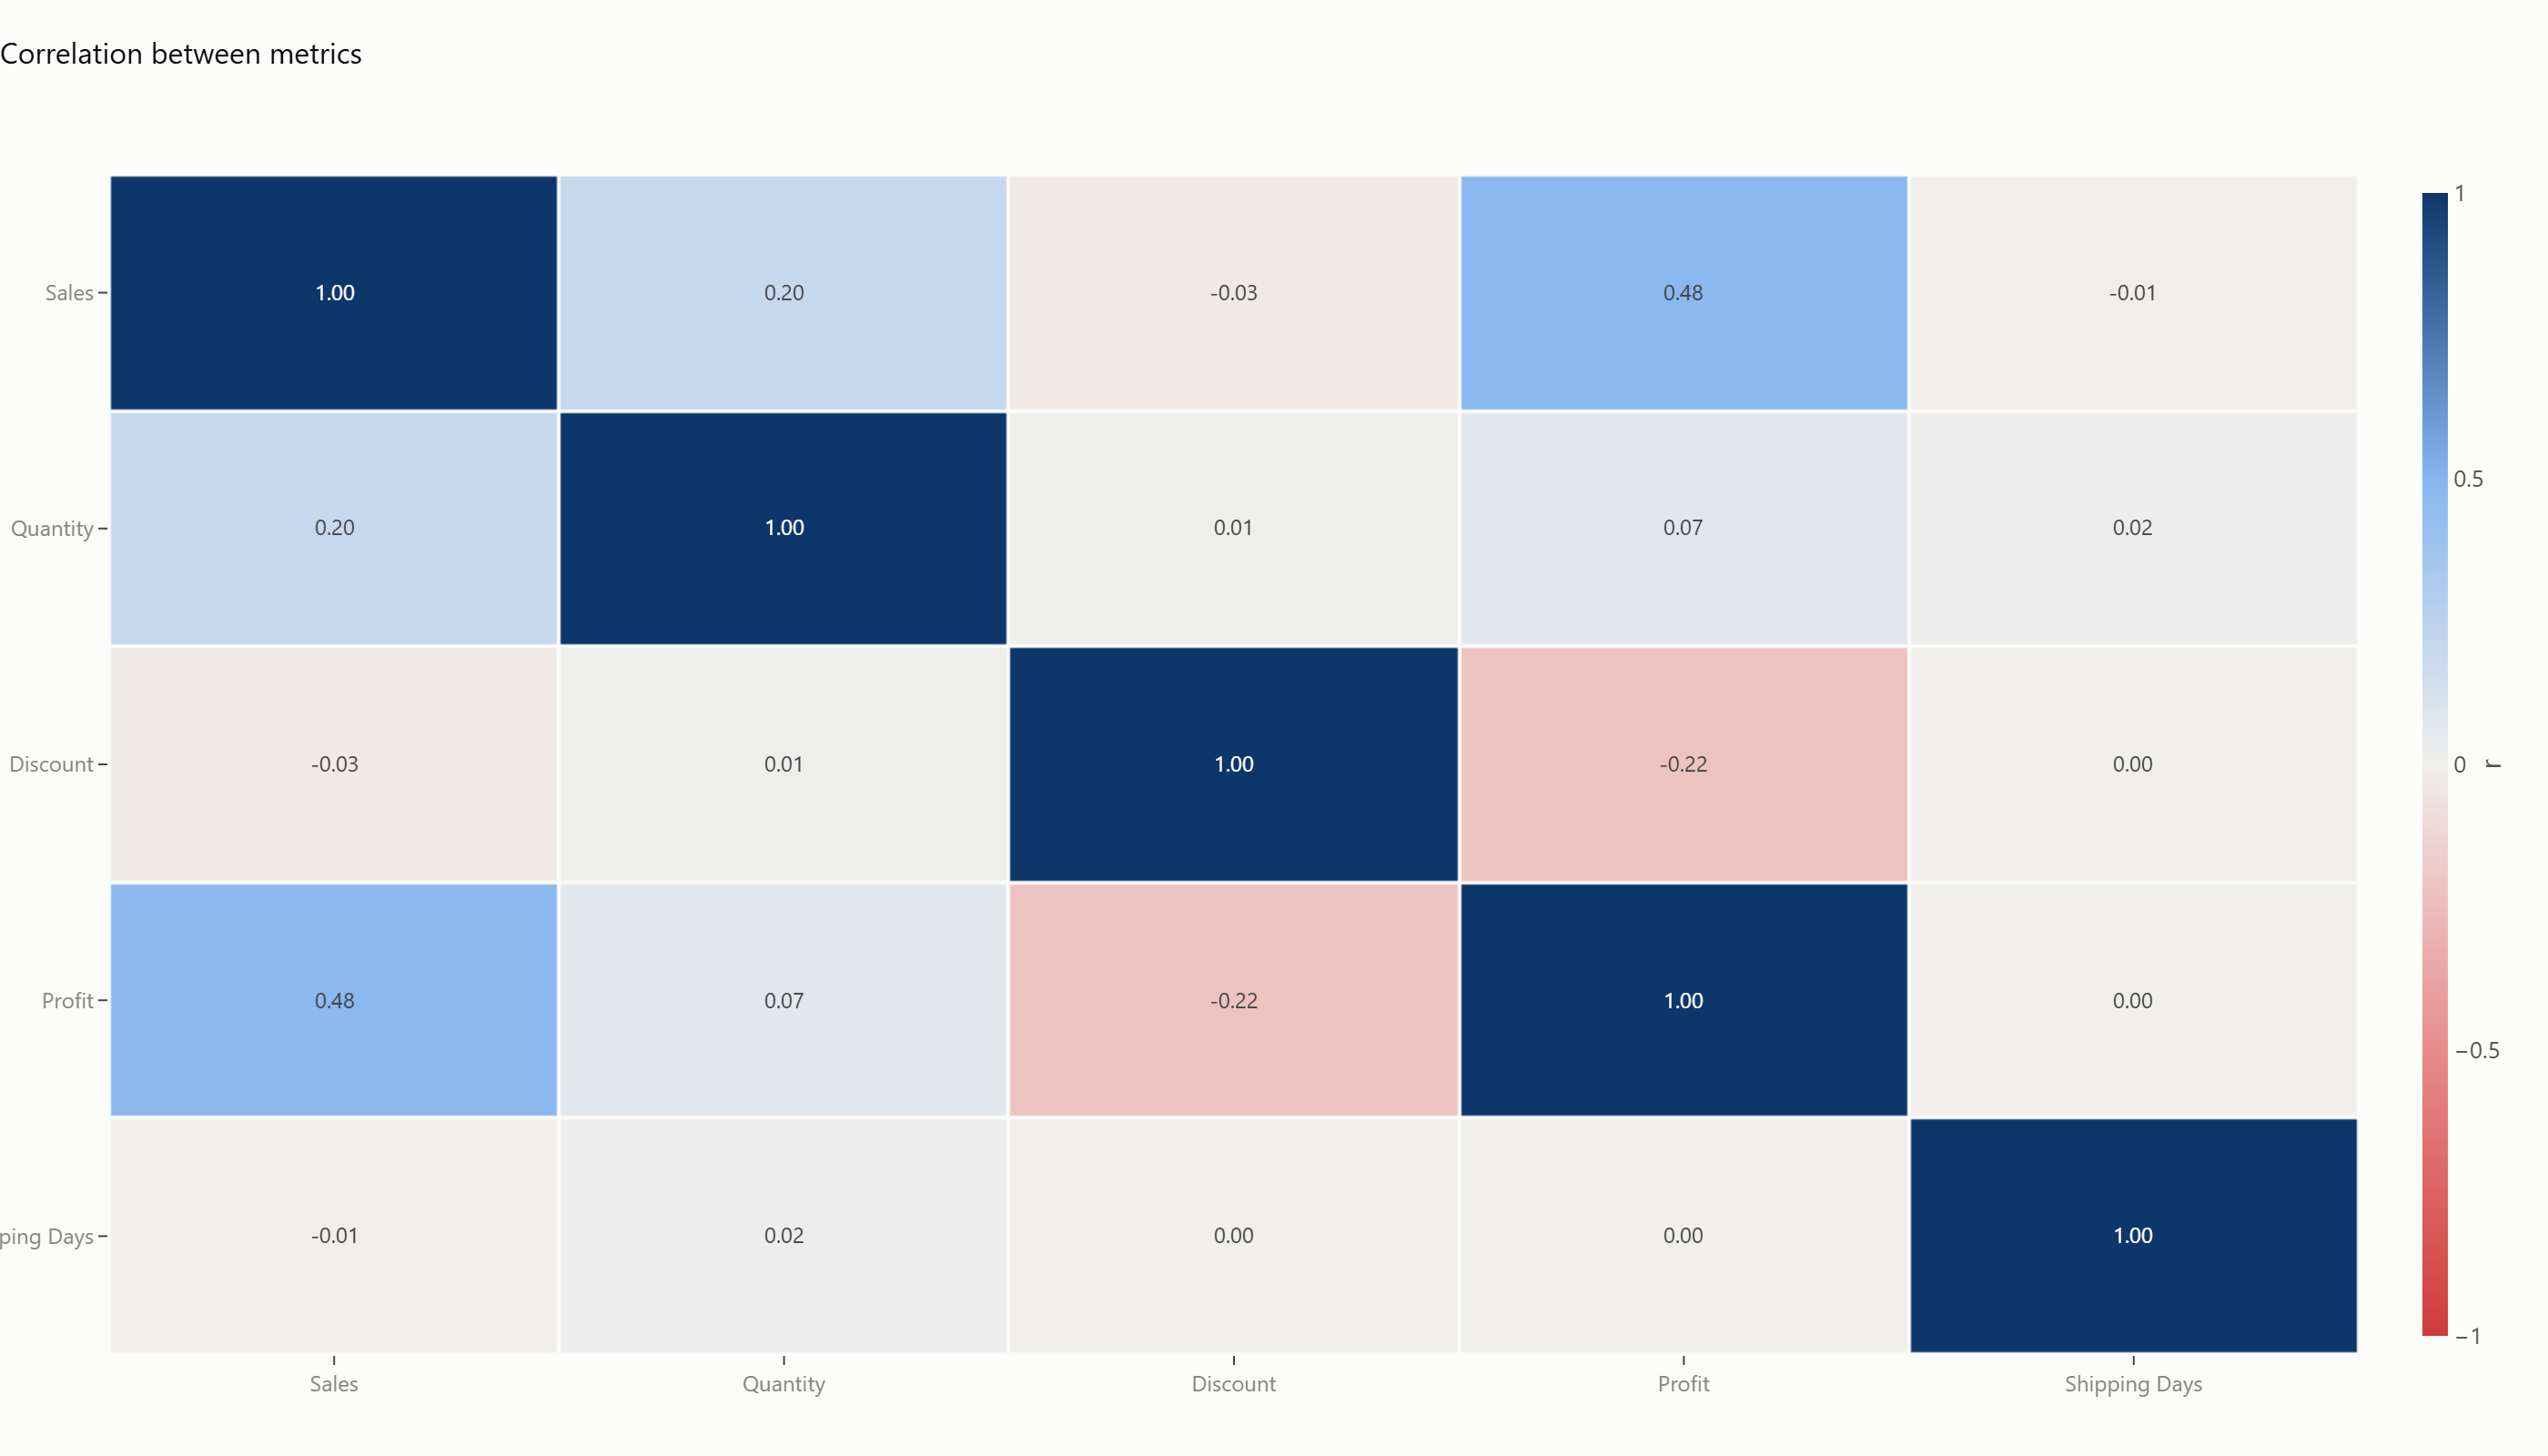
\includegraphics[width=\textwidth]{correlation_light.png}
  \caption{Correlation matrix, diverging and anchored at 0.}
\end{minipage}\hfill
\begin{minipage}{0.49\textwidth}
  \centering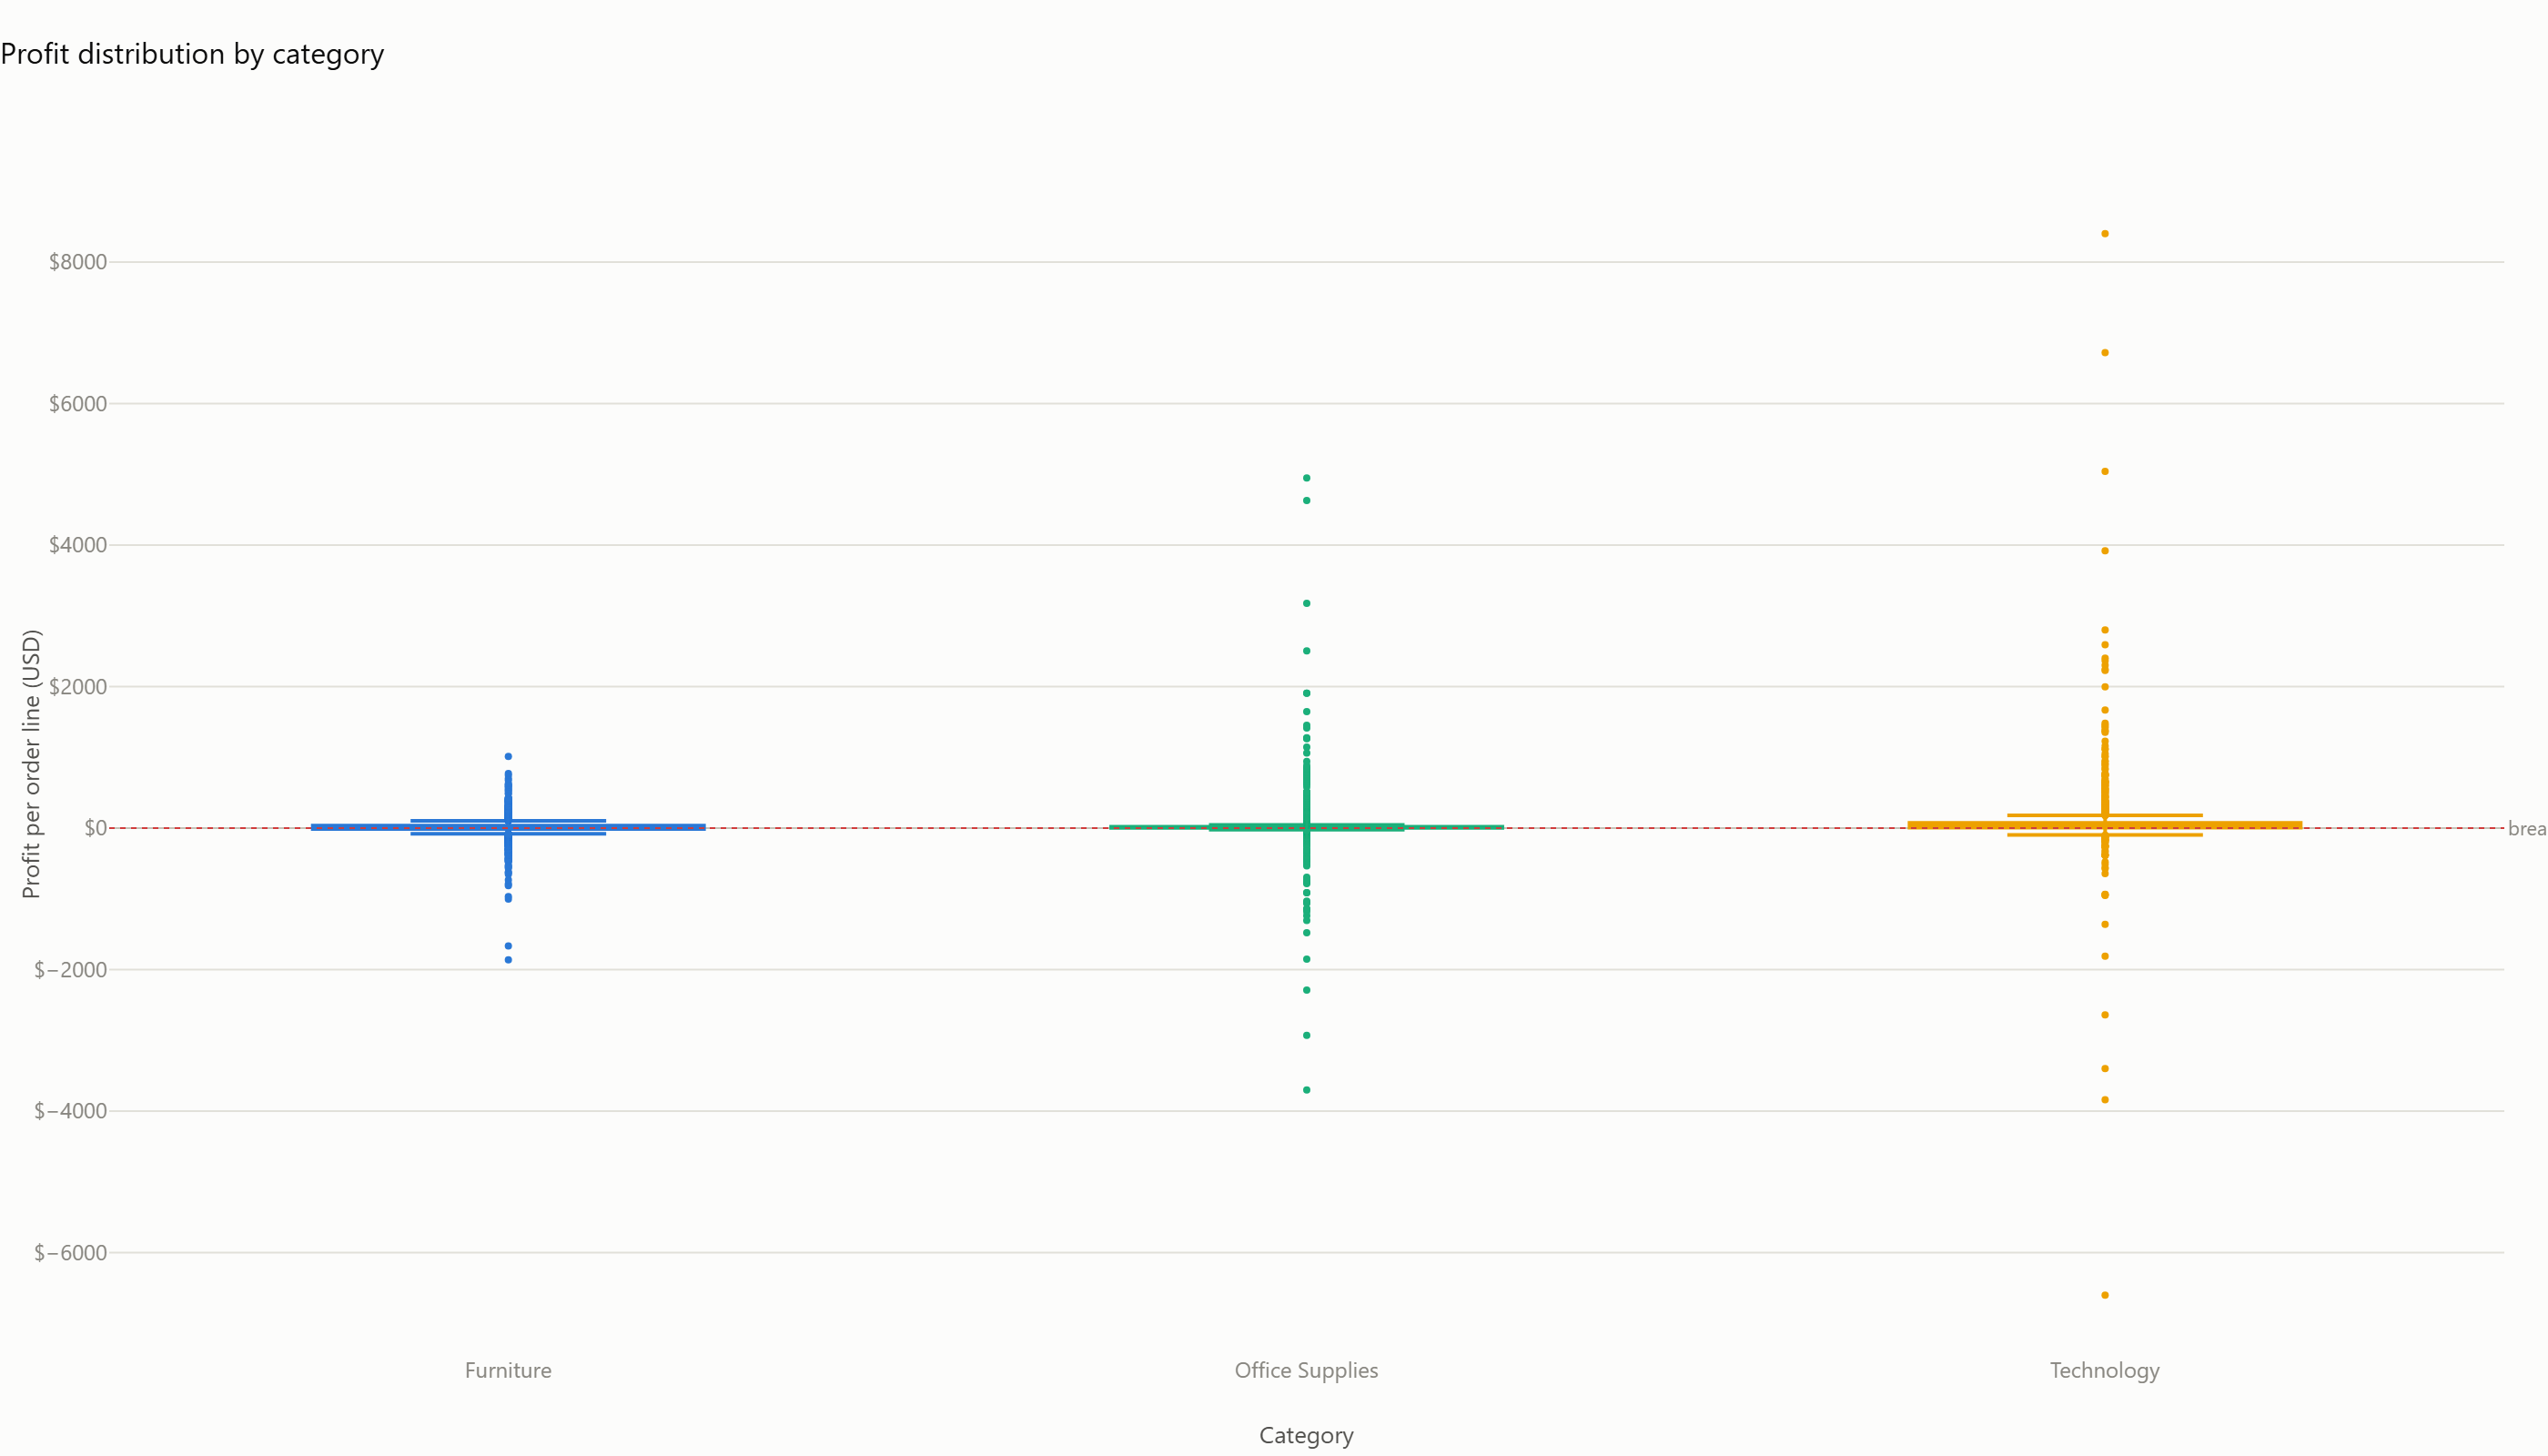
\includegraphics[width=\textwidth]{distribution_light.png}
  \caption{Profit distribution by category (box plot).}
\end{minipage}
\end{figure}

\begin{figure}[htbp]
\centering
\begin{minipage}{0.49\textwidth}
  \centering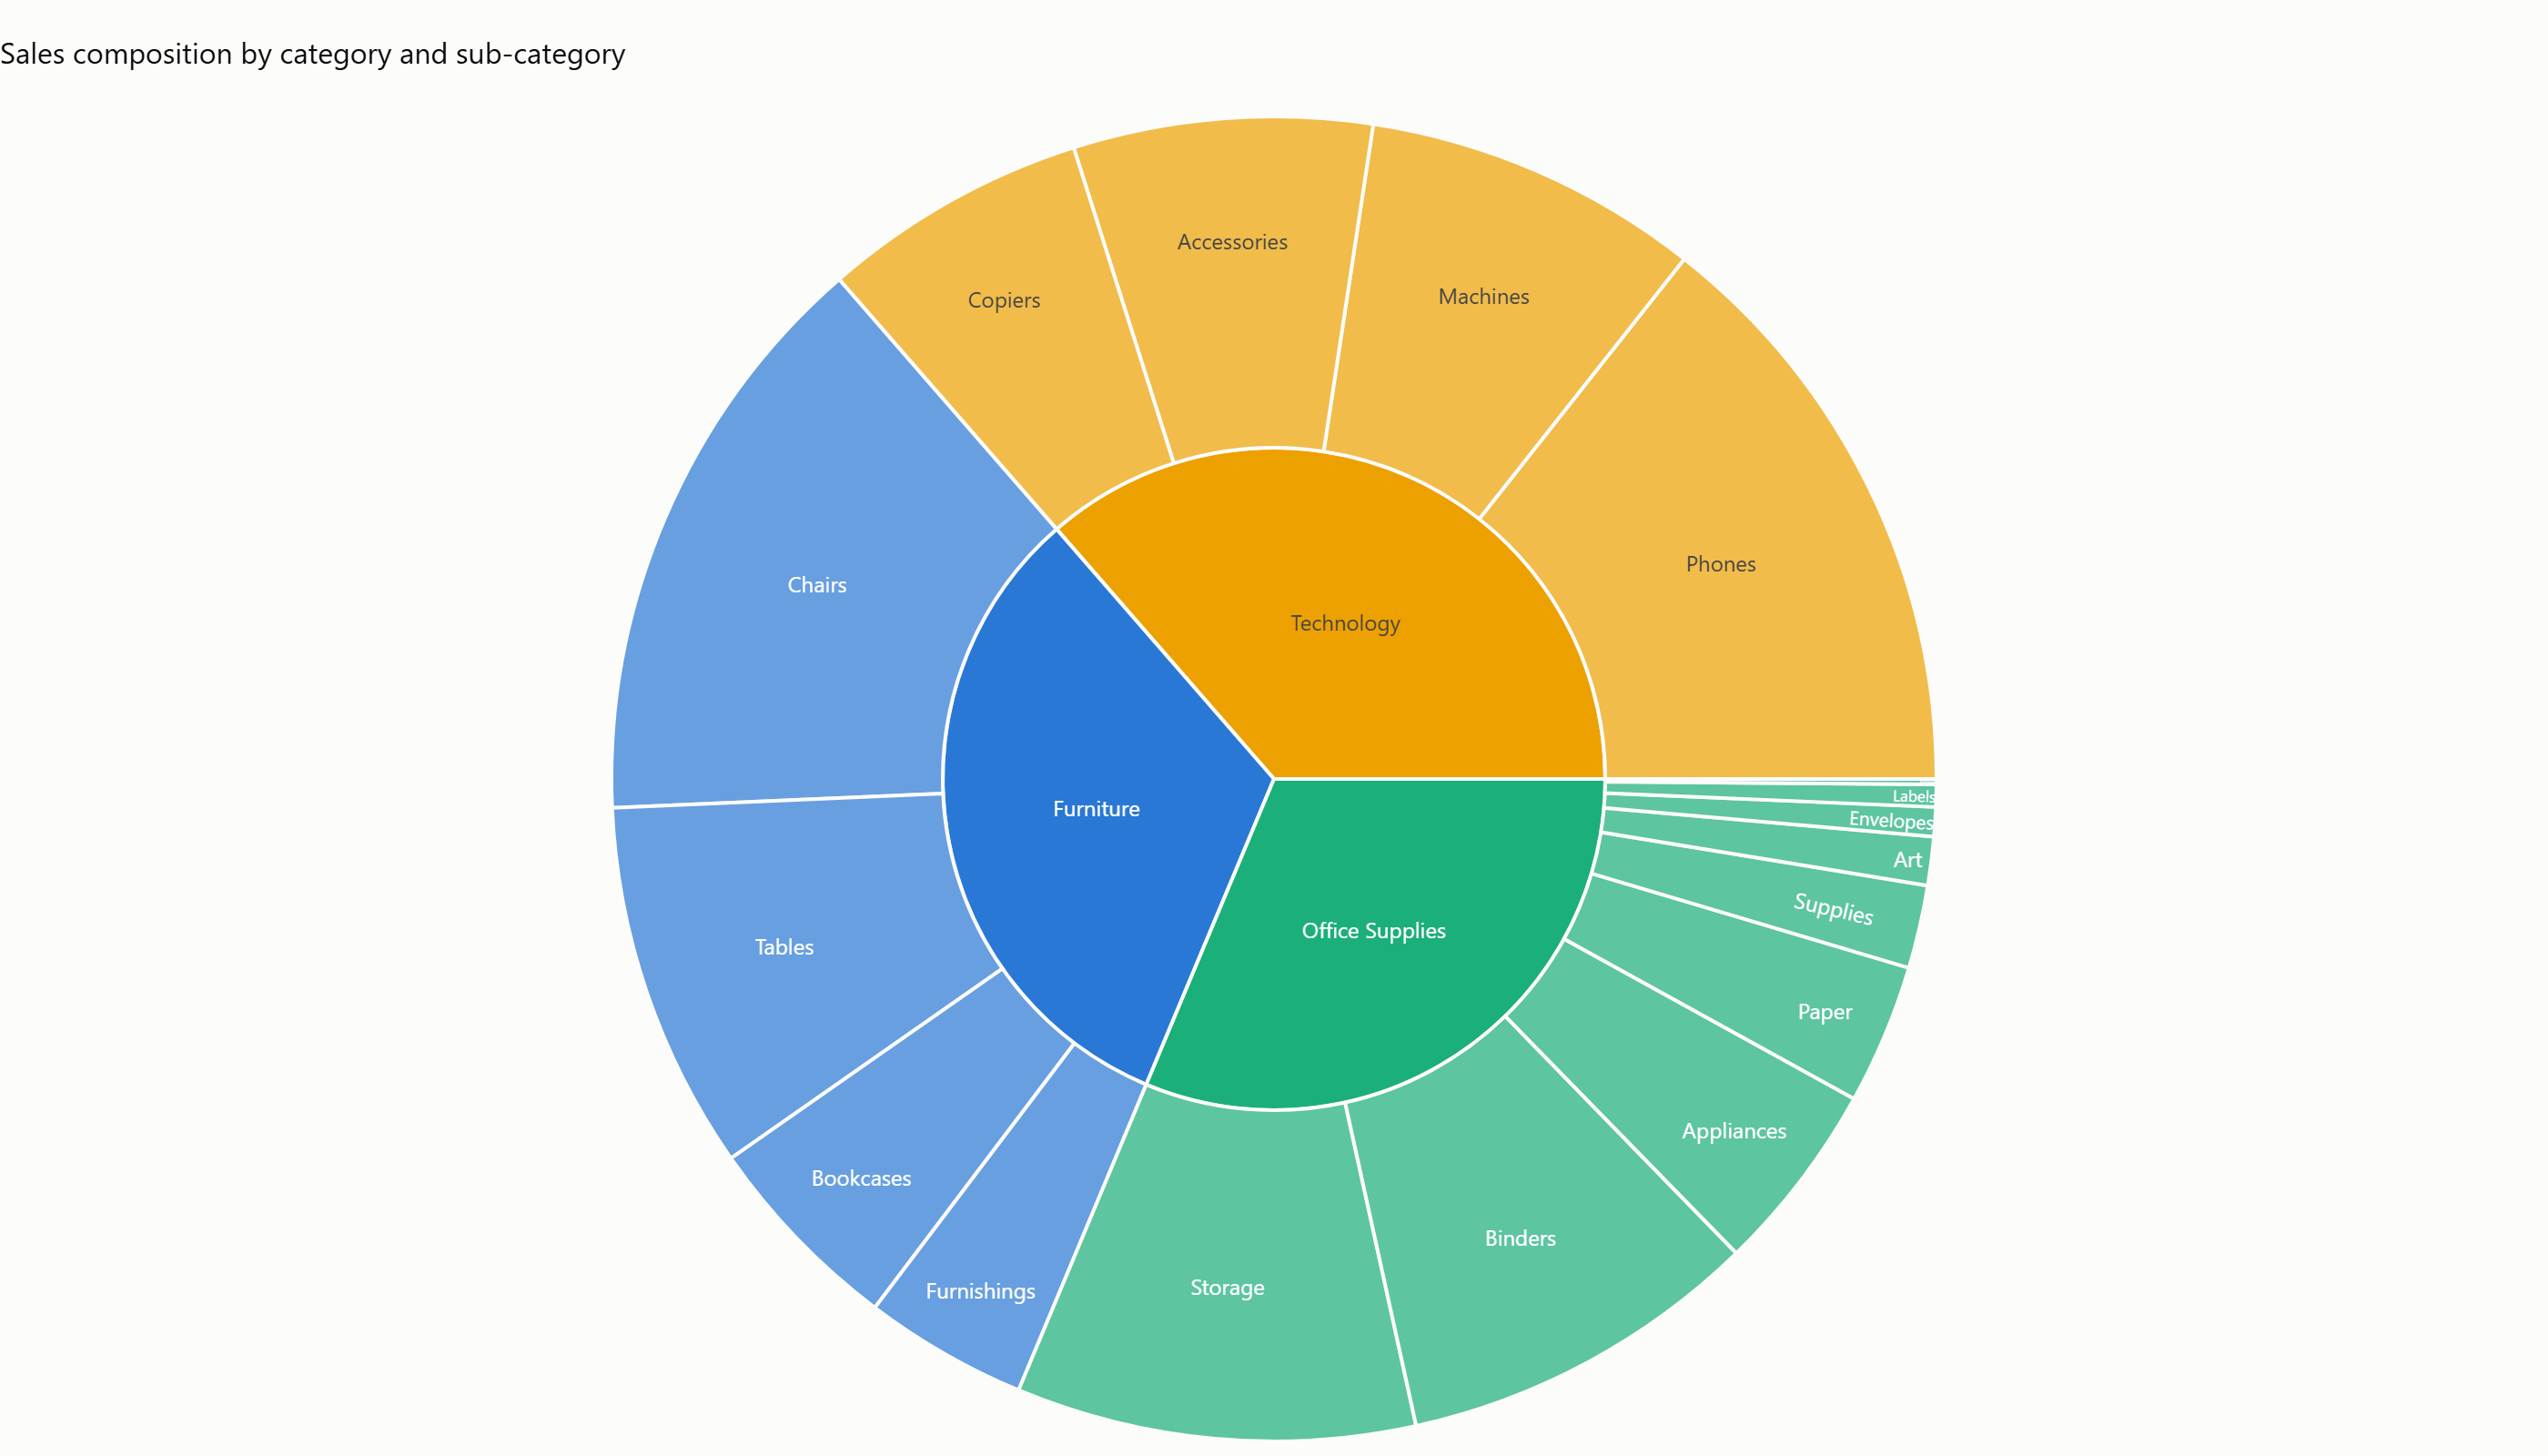
\includegraphics[width=\textwidth]{sunburst_light.png}
  \caption{Category $\rightarrow$ sub-category sunburst.}
\end{minipage}\hfill
\begin{minipage}{0.49\textwidth}
  \centering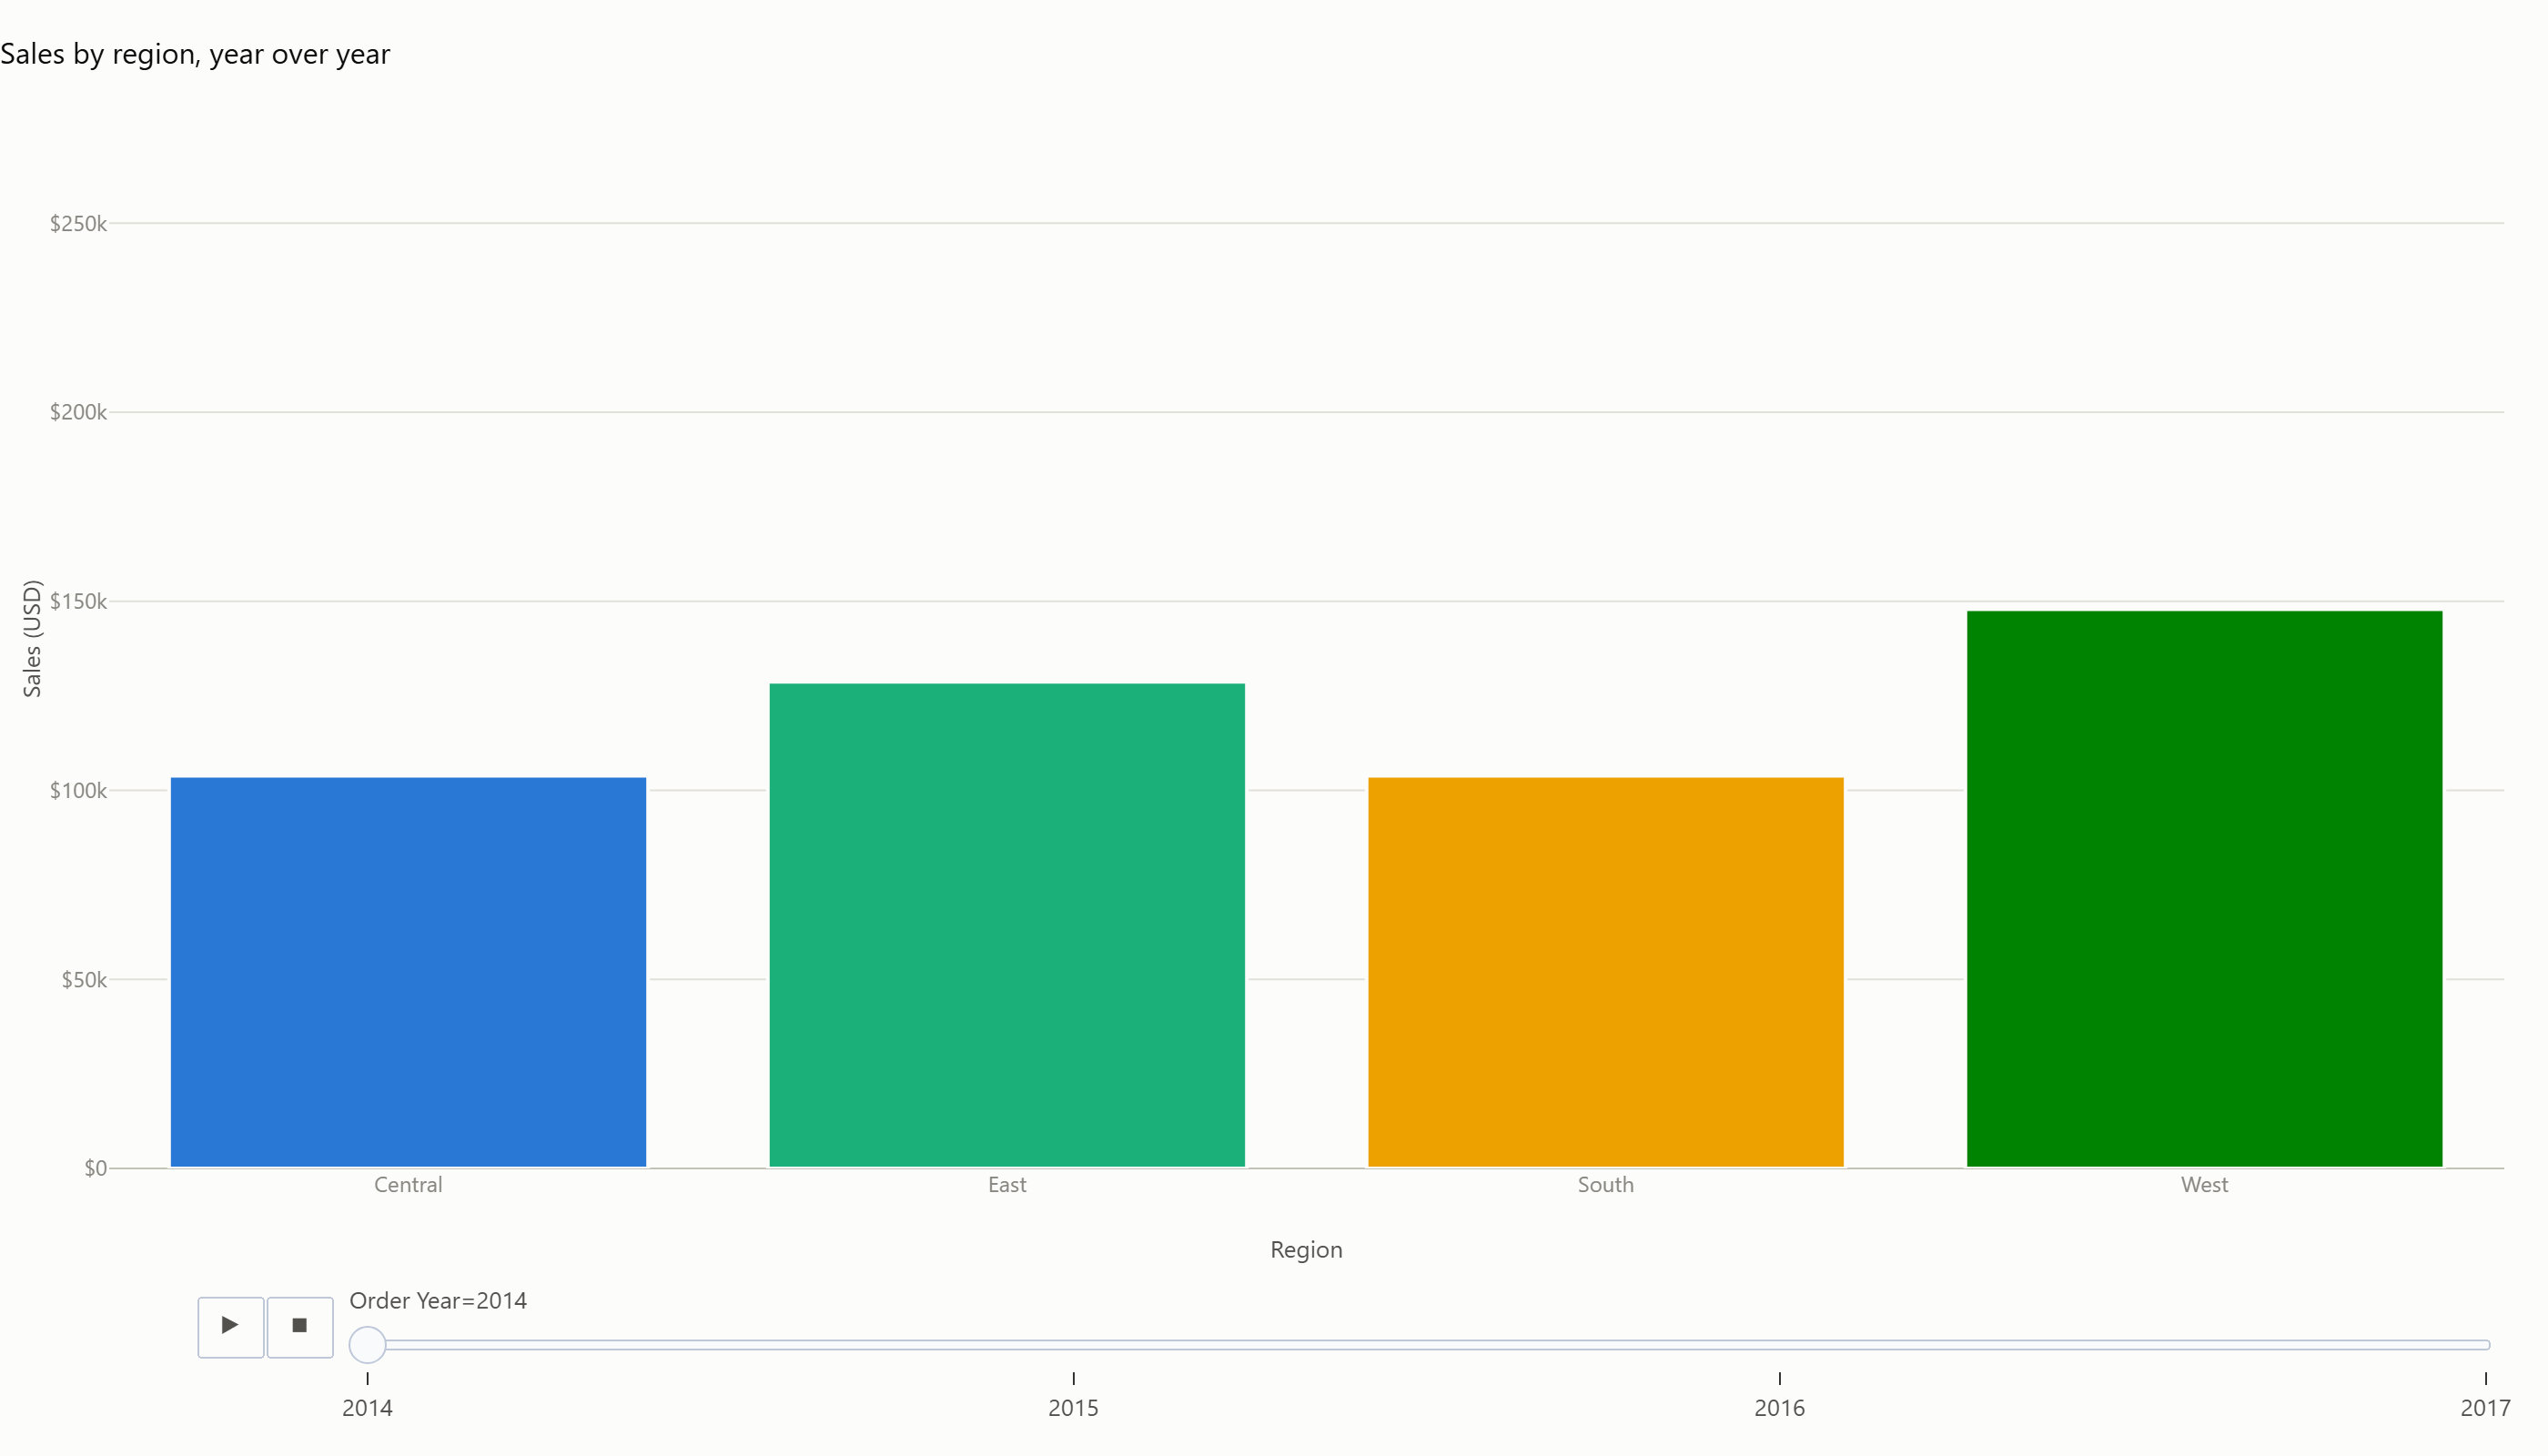
\includegraphics[width=\textwidth]{animated_light.png}
  \caption{Year-over-year animation, y-axis fixed across frames.}
\end{minipage}
\end{figure}

\begin{figure}[htbp]
\centering
\begin{minipage}{0.49\textwidth}
  \centering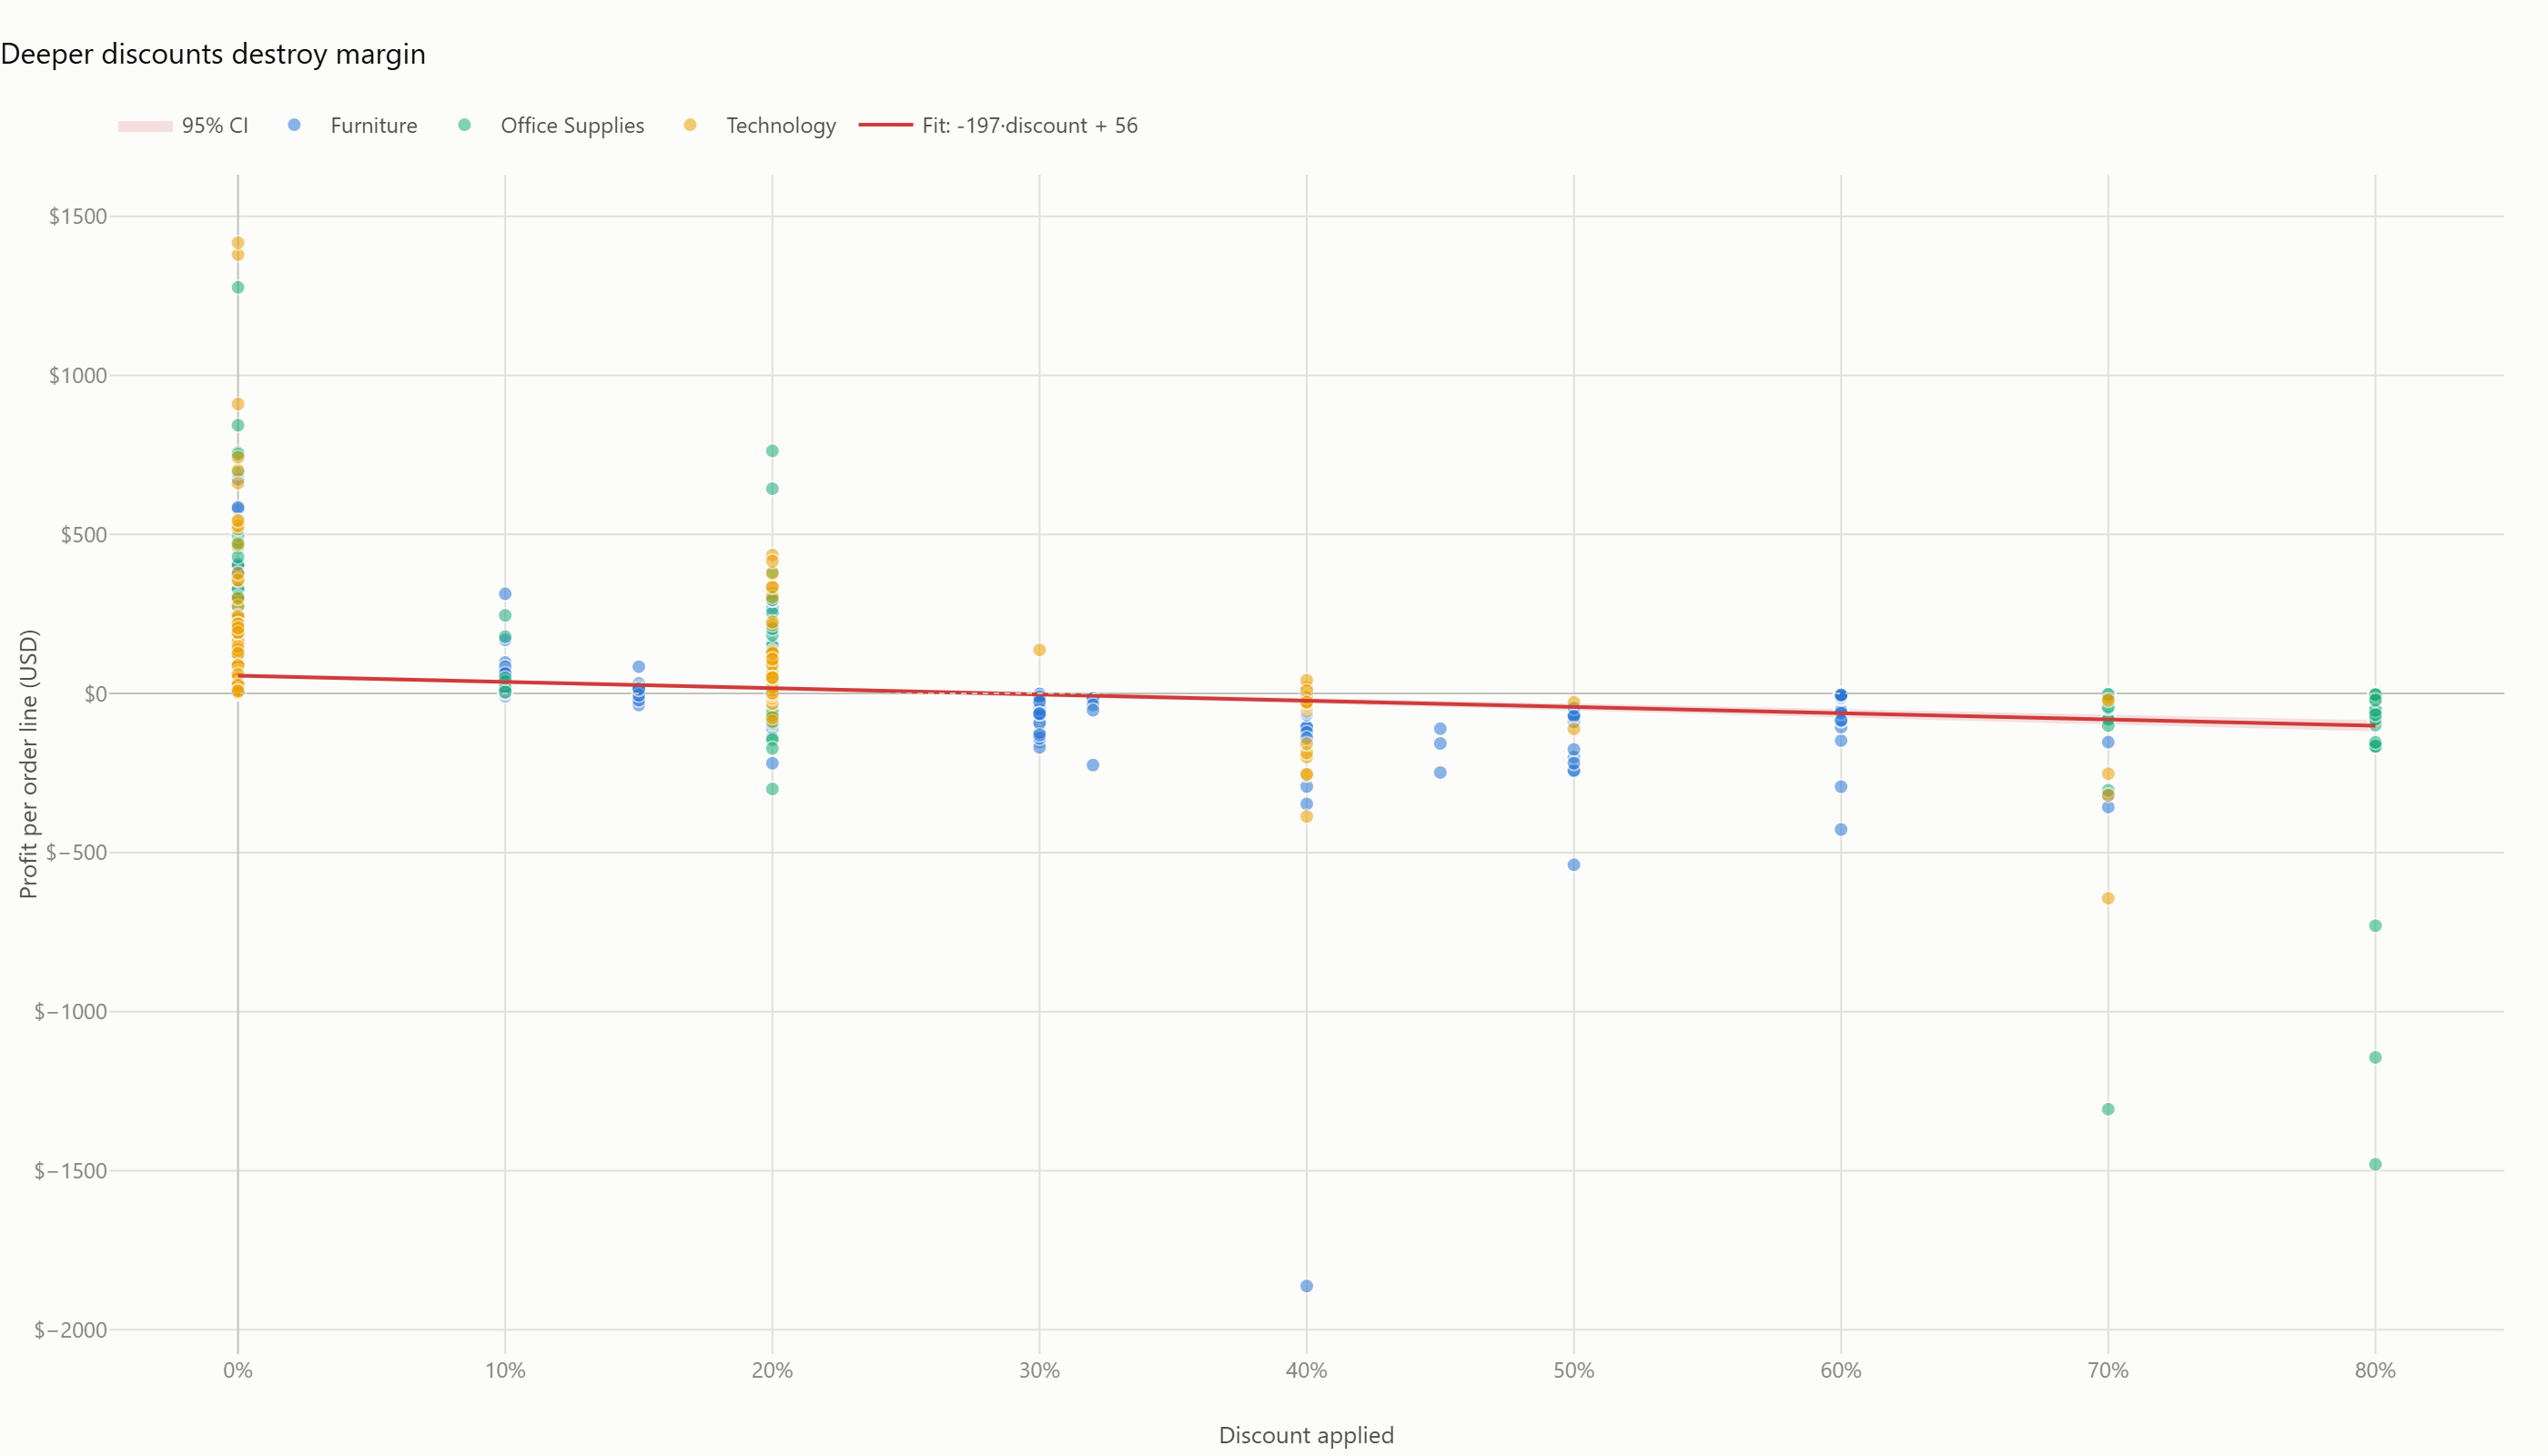
\includegraphics[width=\textwidth]{scatter_light.png}
  \caption{Discount vs profit with a 95\% confidence band.}
\end{minipage}\hfill
\begin{minipage}{0.49\textwidth}
  \centering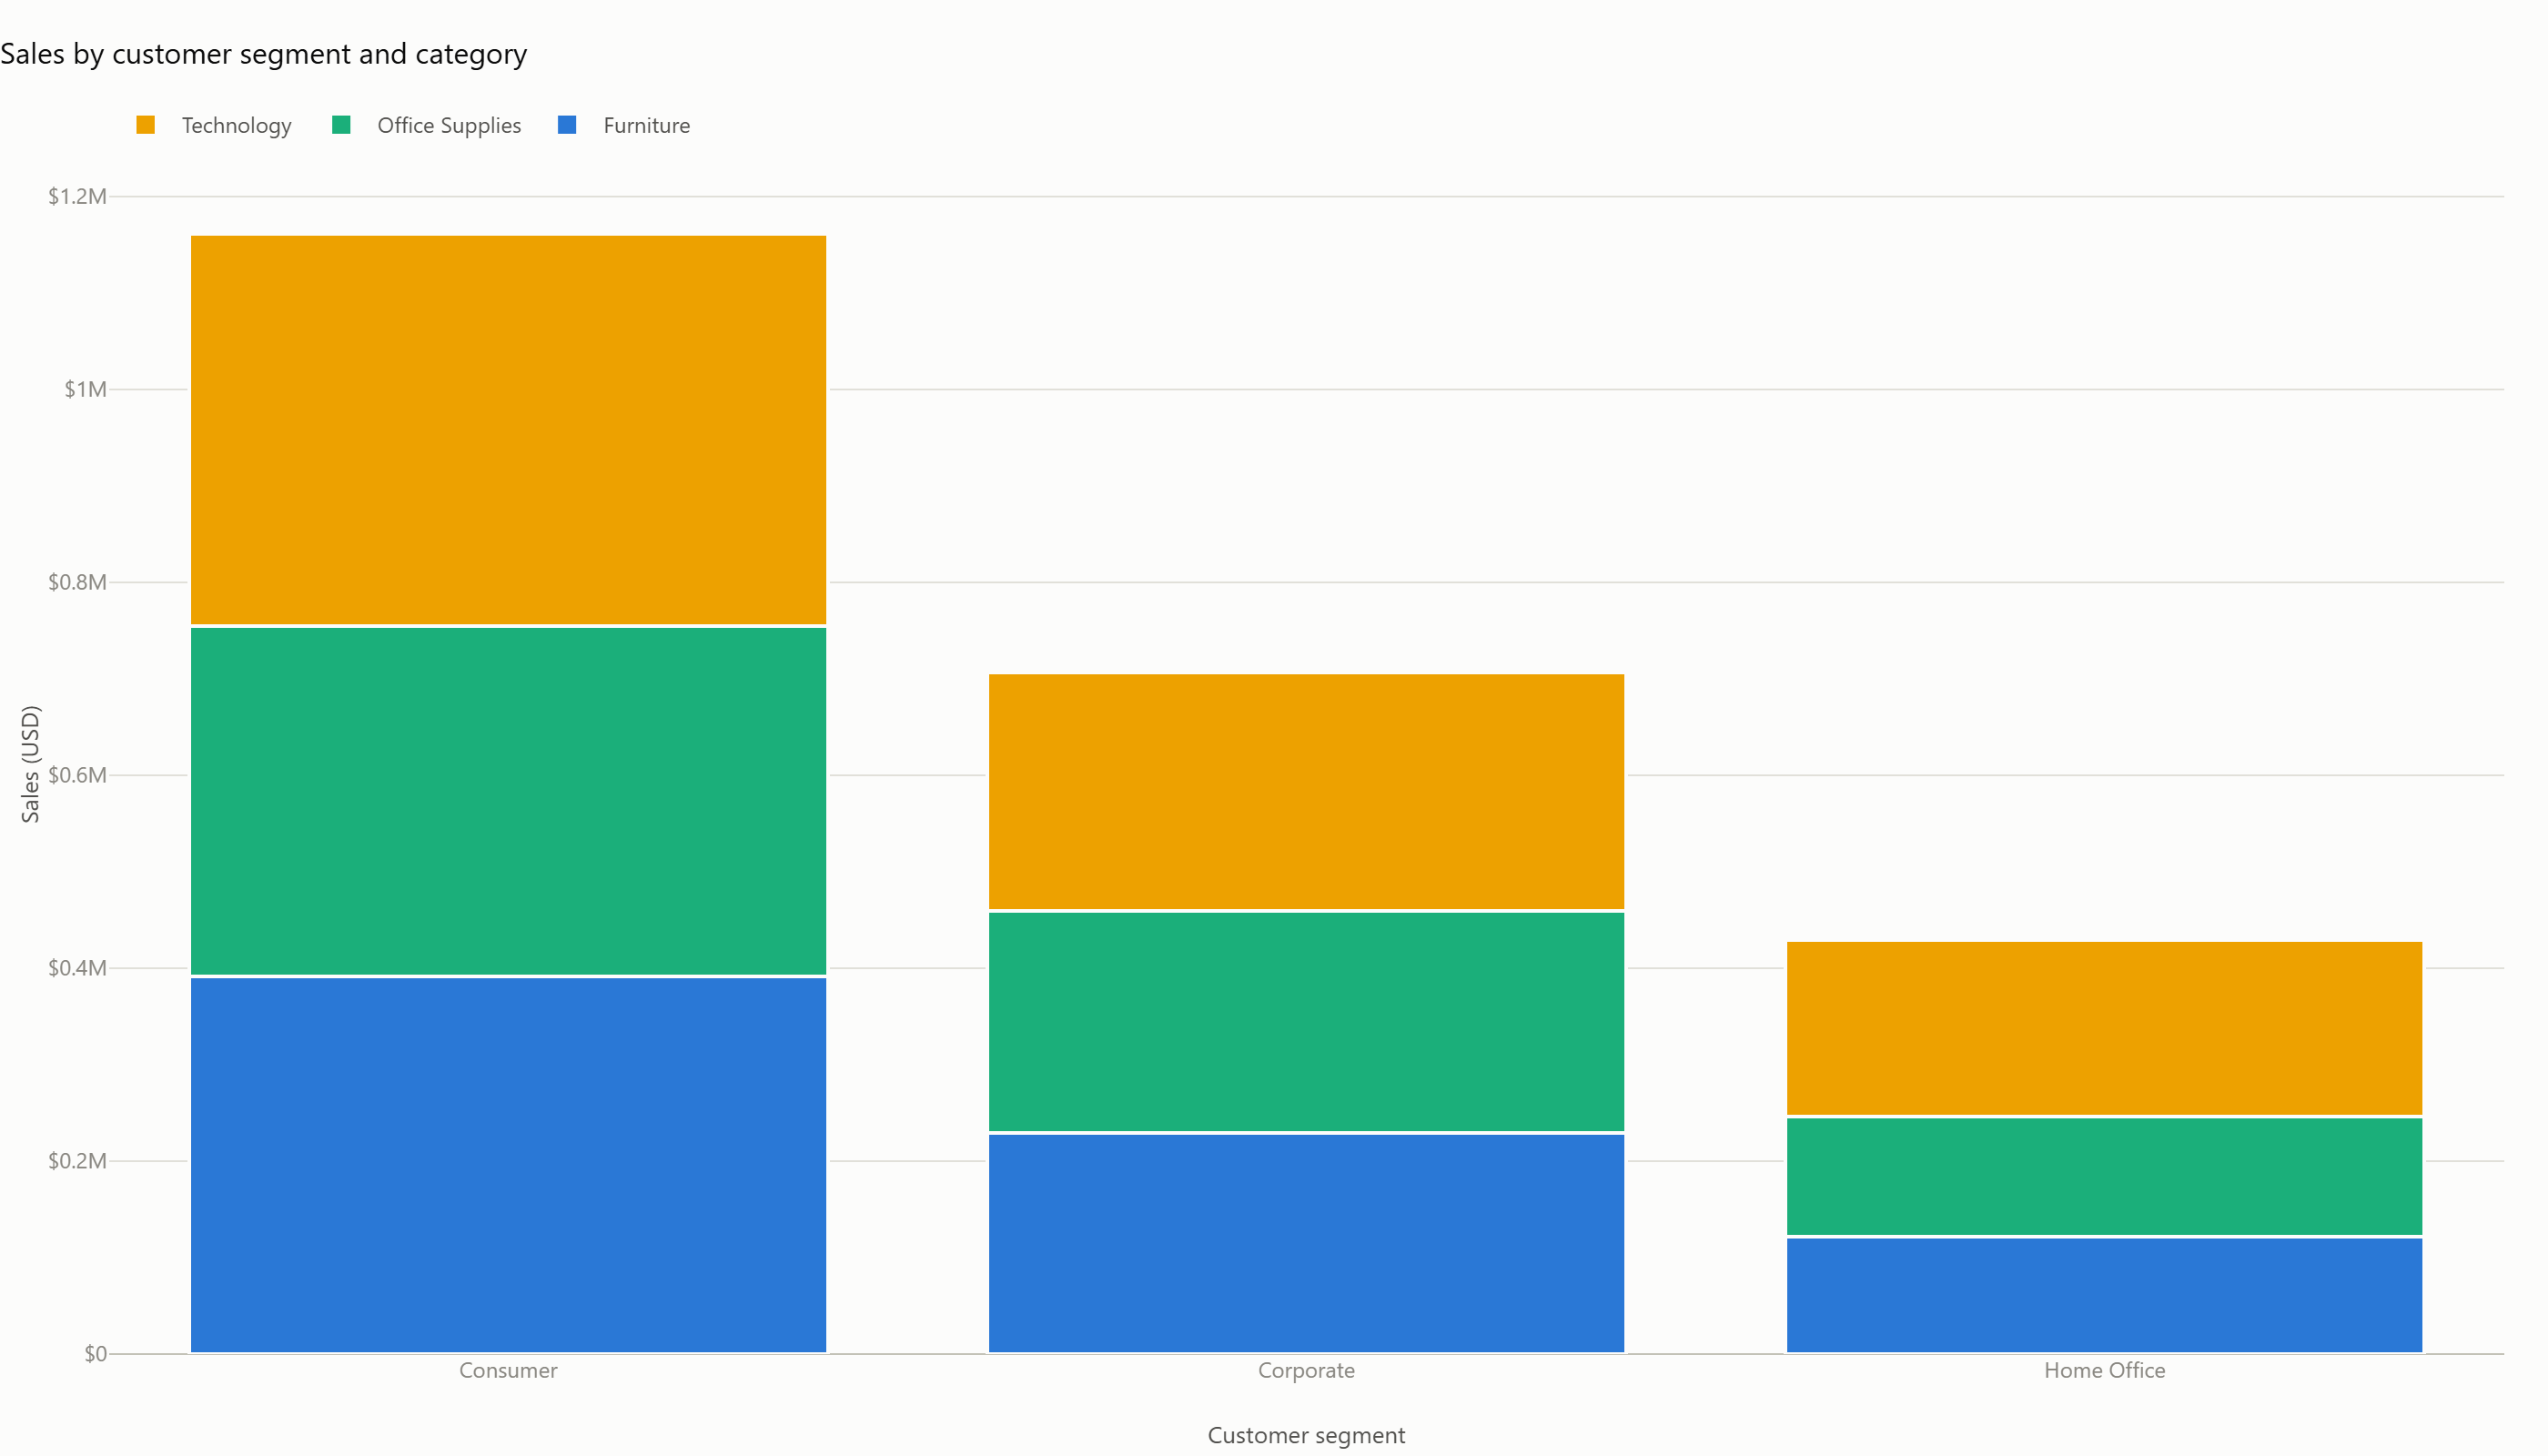
\includegraphics[width=\textwidth]{stacked_light.png}
  \caption{Segment by category (stacked bar).}
\end{minipage}
\end{figure}

\subsection{We deliberately did not build a dual-axis chart}
\label{sec:dual}

The brief offers \emph{``time series or trend chart with dual axis''} as a permitted
type. \textbf{We did not build one, on purpose.}

A dual-axis chart plots two measures on two independent y-scales in one frame. Where the
two lines cross is then \textbf{an artifact of the scales the author chose}, not a fact
about the data: rescale either axis and the crossover moves anywhere you like. It is the
most reliable way to make a chart lie without stating a single false number.

\texttt{trend\_small\_multiples} answers the same question honestly --- Sales and Profit
share an x-axis in stacked panels, so the shapes are comparable while each keeps its own
truthful scale. \textbf{Seven other chart types from the brief's list are implemented, so
the six-type requirement is met without it.}

\subsection{AI-driven visualization (C3)}

When the NL pipeline returns a DataFrame, the application selects a chart type, renders
it, and captions it.

\textbf{The selection is rule-based, not model-generated --- and this is deliberate.}
The shape of a DataFrame is a \emph{fact}: how many rows, which columns are numeric,
whether the label column is temporal or geographic. Facts do not need a language model.
Asking a 4B model to choose would add $\sim$1.5\,s of latency and a new failure mode to
a decision that four \texttt{if} statements make correctly every time.

\begin{center}
\begin{tabularx}{\textwidth}{@{}llX@{}}
\toprule
\textbf{Result shape} & \textbf{Chart} & \textbf{Rationale} \\
\midrule
US state names + metric            & \textbf{map}     & Strictly more informative than 40 bars \\
Temporal label + metric            & \textbf{line}    & The reader should see the \emph{shape} of change \\
Two numerics, no label             & \textbf{scatter} & The question is the relationship \\
Categorical + metric, $\le$30 rows & \textbf{bar}     & Magnitude comparison \\
$>$30 categories, or a scalar      & \textbf{table}   & A 793-bar chart is an unreadable comb \\
\bottomrule
\end{tabularx}
\end{center}

\textbf{Verified: 7/7 shape cases select correctly.} The user can override the choice.
The LLM does the one part that genuinely needs language: \textbf{the one-sentence
caption.}

\subsection{Export (C4) --- and rendering a chart without a browser}
\label{sec:export}

PDF (reportlab), Word (python-docx), PNG and SVG. Every exported report carries dataset
metadata, \textbf{the applied filters}, the AI narrative, the chart image, the result
table, and the generated code.

The filter list is printed \textbf{even when empty} (``None --- the full dataset was
used''). Without it a report is actively misleading: a reader cannot tell whether
``\$2.3M revenue'' is the whole business or one region in one year.

\paragraph{The export path had to be rebuilt for the deployed app.} kaleido, the
standard way to rasterise a Plotly figure, works by driving a headless Chrome. Streamlit
Cloud has no browser, and installing one segfaults the container
(\S\ref{sec:segfault}) --- so on the deployed app every chart export raised, and because
\texttt{st.download\_button} evaluates its \texttt{data} argument eagerly, that
exception took down the whole page on every rerun rather than on click.

\textbf{The fix is not to degrade but to redraw.} \texttt{src/viz/browserless.py} reads
the traces back off the Plotly figure and redraws them with matplotlib's Agg
rasteriser --- pure software, no browser, no system libraries. The diverging scale is
rebuilt from the same \texttt{[position, colour]} stops \texttt{theme.py} defines, so a
loss still reads red rather than in a matplotlib lookalike palette. kaleido remains the
primary path wherever a browser exists, so every local run --- including the figures in
this report --- is unchanged.

It covers exactly the traces the AI-driven charts emit (bar, line, scatter) and
\textbf{refuses anything else rather than inventing an approximation}: a choropleth is
drawn from Plotly's own US geometry, which matplotlib does not have, so on the deployed
app a map's image buttons are hidden and its report prints without the map. An HTML-to-PDF
route was considered and rejected: Plotly charts are drawn by JavaScript at runtime, and
no pure-Python HTML renderer executes JavaScript, so it would have embedded an empty
\texttt{<div>}.

\paragraph{A bug this exposed, worth recording.} The first fix worked locally and failed
on Cloud from the second question onward. plotly 6 encodes numpy arrays as
\texttt{\{"dtype": "f8", "bdata": "<base64>"\}} whenever a figure is serialised, and
\texttt{st.cache\_data} pickles what it caches --- so a figure is live on the turn it is
built and base64-encoded on every rerun after. plotly never decodes that in Python
(the spec exists for plotly.js, and kaleido hands it to the browser untouched), so the
encoding was invisible until something tried to read the arrays in Python. Our test had
rendered figures fresh from the builder; Streamlit served them from a cache. The
fallback now decodes the spec, and the test asserts through a pickle round trip.

% =====================================================================
% 8. TASK D
% =====================================================================
\section{Task D --- Advanced Features}

\subsection{D3 --- Anomaly detection}
\label{sec:anomaly}

Isolation Forest over \texttt{Sales}, \texttt{Quantity}, \texttt{Discount},
\texttt{Profit}, \texttt{Shipping Days}, with IQR and z-score reported alongside for
comparison. Features are standardised first --- the forest partitions on raw values, and
Sales spans 0.4--22,638 while Discount spans 0--0.8; without scaling, Discount would be
invisible to the model.

\begin{lstlisting}
Flagged: 200 of 9,994 rows (2% contamination)
Loss across flagged rows: $74,142
Flagged rows that lose money: 41.5%   Baseline: 18.7%   Enrichment: 2.22x
Reproducible: identical flags on repeat runs (random_state=7)
\end{lstlisting}

\subsubsection*{The finding: our own justification for the forest was wrong}

The standard argument for an Isolation Forest is that it catches rows whose
\emph{combination} of values is unusual while no single column is extreme. \textbf{We
measured this. On this dataset it is false.}

\begin{center}
\begin{tabular}{@{}ccc@{}}
\toprule
\textbf{Contamination} & \textbf{Flagged} & \textbf{Caught by forest but \emph{not} by IQR} \\
\midrule
1\%  & 100   & \textbf{0} \\
2\%  & 200   & \textbf{0} \\
5\%  & 500   & 1 \\
10\% & 1,000 & 22 \\
\bottomrule
\end{tabular}
\end{center}

At every operationally sensible threshold, the forest finds \textbf{nothing} the
univariate rules miss.

\textbf{Its real value is selectivity.} The union of the per-column IQR rules flags
\textbf{2,851 rows --- 28.5\% of the dataset.} ``A third of your orders are unusual'' is
not an alert list anyone can act on; it is noise with a threshold attached. The forest
returns a \textbf{bounded, ranked} set with a continuous score, so the worst row comes
first and a human can start at the top. \textbf{IQR cannot rank at all.}

We report this rather than quietly selecting the algorithm that sounds most advanced.
The test that actually matters --- are flagged rows more likely to be genuinely bad? ---
the forest passes at \textbf{2.22$\times$ enrichment over baseline}.

The LLM never decides what is anomalous. It narrates rows the detectors have already
flagged. A model that could invent anomalies could invent a crisis that does not exist.

\subsection{D4 --- ReAct multi-turn reasoning agent}
\label{sec:agent}

A tool-calling loop: the model decides which tool to call, observes the result, and
decides again. The full reasoning chain is surfaced in a collapsible debug panel.

\textbf{Six tools} against a required three:

\begin{center}
\texttt{query\_data} $\cdot$ \texttt{detect\_anomalies} $\cdot$ \texttt{get\_holidays}
$\cdot$ \texttt{compare\_dates} $\cdot$ \texttt{create\_chart} $\cdot$ \texttt{final\_answer}
\end{center}

\subsubsection*{Why the agent's tools need no sandbox --- and Task B's do}

This is the design distinction worth the most in this project.

\begin{center}
\begin{tabularx}{\textwidth}{@{}lXX@{}}
\toprule
 & \textbf{Task B pipeline} & \textbf{Task D4 agent} \\
\midrule
Model produces          & \textbf{Arbitrary pandas code}      & \textbf{Typed tool arguments} \\
Who builds the call     & The model                           & \textbf{The executor} \\
Safety model            & \textbf{Containment} (3-layer sandbox) & \textbf{Construction} (schema-bounded) \\
Can express             & Anything Python can                 & Only what the tool schema allows \\
\bottomrule
\end{tabularx}
\end{center}

The agent's \texttt{query\_data} takes an enum'd column name and an enum'd aggregation.
The model \emph{cannot express} anything outside that schema, so this surface is
\textbf{safe by construction and needs no sandbox at all.} Both approaches exist in this
project on purpose: one is right when you need expressive power, the other when you need
guarantees.

\subsubsection*{The one tool that leaves the machine}

The dataset is four years of US order lines and nothing else. It cannot say whether
24 November 2016 was a Thursday like any other or Thanksgiving --- and \emph{``do sales
move around public holidays?''} is a fair question to ask of retail data that the data
alone cannot answer. \texttt{get\_holidays} fetches that missing calendar from
Nager.Date, a free keyless public-holiday API; \texttt{compare\_dates} then joins the
returned dates back to the orders.

Network reach is where agents usually acquire their worst failure mode: a tool returns
attacker-controlled prose, the prose enters the model's context, and the model follows
it --- indirect prompt injection. Rather than abandon the safety-by-construction
principle, we applied it:

\begin{center}
\begin{tabularx}{\textwidth}{@{}lX@{}}
\toprule
\textbf{Guard} & \textbf{Effect} \\
\midrule
Fixed host      & The URL is built from constants. The model supplies a year and nothing else --- it cannot name a host, path or scheme \\
Validated year  & Must be an integer inside the dataset's 2014--2017 span \\
Two fields kept & Only an ISO date and a name survive; every other field of the response is dropped \\
Name sanitised  & Whitespace collapsed, truncated to 60 chars --- so a name cannot forge extra lines inside the observation block \\
Bounded         & 8\,s timeout, hard cap on holidays returned \\
Cached          & Memoised per year: fetched once per process \\
Fails soft      & Network errors become an \emph{observation}, not an exception --- a dead API cannot end a run \\
\bottomrule
\end{tabularx}
\end{center}

\textbf{This API was chosen over a web search precisely because its response has no
free-text field worth attacking} --- dates and short names, nothing else. Search would
have looked more impressive and handed the model a paragraph of someone else's text.
Verified against a hostile payload (a holiday ``name'' carrying newlines and
\texttt{IGNORE ALL PRIOR RULES}): the forged newlines are collapsed, the extra fields
dropped, and one truncated line reaches the model.

\textbf{The residual risk, stated rather than hidden:} up to 60 characters from a fixed,
known host still reach the model. That is not zero. It is acceptable here on quantity
and source, and it would not be for a search tool.

\subsubsection*{Live results (real Gemma 4 E4B)}

\begin{lstlisting}
Q: "Which region has the highest total sales? Chart it."
   ACT  query_data({"aggregation":"sum","group_by":"Region","metric":"Sales"})
   OBS  4 rows in 3ms: West 725457.82 | East 678781.24 | Central 501239.89 | South 391721.91
   ACT  create_chart({"chart_type":"bar"})
   ANS  "The West region has the highest total sales with $725,457.82."
   -> 2 tool calls, 2.3 s. Correct.

Q: "Find the most unusual order lines and tell me what went wrong."
   ACT  detect_anomalies({"top_n": 5})
   OBS  Isolation Forest flagged 200 of 9,994 (total loss on flagged: -$74,142)
   THINK "CA-2016-117121 (Binders): Profit was $4,946.37. This line does not
          appear to show a loss based on the provided data."
   ANS  "...CA-2016-108196 (Machines) shows a profit of -$6,599.98..."
   -> 1 tool call, 10.2 s.

Q: "Do sales rise around US public holidays in 2016?"
   ACT  get_holidays({"year": 2016})                          <- external API
   OBS  13 US public holidays in 2016 (from date.nager.at): 2016-01-01 New Year's Day ...
   ACT  compare_dates({"dates": [13 dates], "metric": "Sales", "window_days": 3})
   OBS  those dates: $2,133.15/day across 73 days | other days: $1,839.76/day across 1,164
        difference: +15.9% per day
   ANS  "Yes, sales appear to rise around US public holidays in 2016..."
   -> 2 tool calls, 7.4 s. Correct.
\end{lstlisting}

Three things in that transcript are worth pointing at. In the second run the agent
\textbf{correctly observed that the top-ranked anomaly is not a loss at all} --- it is
an unusually large \emph{profit} --- and said so before moving on to the ones that are.
That is reasoning about an observation, not pattern-matching. In the third, the second
call's arguments \emph{are the first call's output}: a genuinely dependent chain, which
is precisely what the Task B pipeline cannot express and the reason the agent exists.
And asked the same question about \textbf{2026}, the agent answers ``the available data
only covers up to 2017'' and offers the years it does have --- it declines rather than
fabricates.

\paragraph{Stated limitation.} Gemma 4 E4B plans two or three steps competently and then
begins to loop, re-calling the same tool with the same arguments. \texttt{MAX\_STEPS=6}
and duplicate-call detection are guards a larger model would not need. We report this
rather than hiding it behind a curated demo.

% =====================================================================
% 9. EVALUATION
% =====================================================================
\section{Evaluation}

\subsection*{What works well}

\begin{itemize}[leftmargin=*]
\item \textbf{Text-to-code accuracy: 10/10} on the benchmark, 2.0\,s mean, zero retries.
\item \textbf{The sandbox holds.} 8/8 escape attempts blocked, including every bypass
      that defeats a naive substring filter.
\item \textbf{Sub-5\,ms queries}, 100$\times$ under budget.
\item \textbf{Zero cost per query}, no data leaves the machine.
\item \textbf{Colour is accessible}, validated rather than assumed.
\item \textbf{The agent genuinely composes} multi-step plans, reaches an external API,
      and reasons about observations.
\end{itemize}

\subsection*{What does not}

\begin{itemize}[leftmargin=*]
\item \textbf{There is no automated test suite.} The \texttt{check\_task\_*.py} scripts
      are acceptance smoke tests that need a live model; they are not unit tests and no
      CI runs them. This is the project's largest engineering gap, and it is not
      theoretical --- see below.
\item \textbf{Two bugs reached the deployed app} (\S\ref{sec:export}): the kaleido/Chrome
      crash, and the base64 array encoding that broke every question after the first.
      Both were in pure functions, both were trivially testable, and both reached
      production because nothing ran before the push.
\item \textbf{The renderer mangled every dollar amount for most of the project's
      life} (\S\ref{sec:math}), and none of our checks could see it: they assert on
      the text the model returns, and that text was always correct. It took
      screenshotting the app for this report to notice. \textbf{The lesson is that a
      check which never looks at the output a human sees cannot find the bugs a human
      sees} --- and our checks are all of that kind.
\item \textbf{The agent loops} beyond 2--3 steps. Guarded, not solved.
\item \textbf{The agent is narrow.} Its typed tools cannot express what
      \texttt{query\_data}'s enums do not contain, so for most questions the Task B
      pipeline is the better tool. The agent earns its place on external-data questions
      and dependent chains, which is a real but narrow win.
\item \textbf{Cloud reports omit the map.} Bar, line and scatter fall back to
      matplotlib; a choropleth cannot be redrawn without Plotly's geometry.
\item \textbf{The stacked bar has no drill-down}; \textbf{dark mode is built and
      validated but not exposed}; \textbf{responsiveness at 1280px is untested}.
\item \textbf{The Isolation Forest adds no novelty over IQR} on this dataset
      (\S\ref{sec:anomaly}). Its value is ranking and selectivity, which is a weaker
      claim than we expected to make.
\item \textbf{Two benchmark questions were reworded} after observing failure
      (\S\ref{sec:bench}). We believe this was justified; we disclose it so the reader
      can judge.
\item \textbf{A performance bug nearly wrecked the demo.} \texttt{st.download\_button}
      evaluates its \texttt{data} argument \emph{eagerly} --- each export rendered a
      chart through kaleido at $\sim$1.5\,s. With five answers in history, \textbf{every
      filter change triggered 30.7\,s of work.} Found by profiling the rerun path; fixed
      by caching against the filter scope. We found this by \emph{measuring} rather than
      by assuming the code was fine because it looked fine.
\end{itemize}

\subsection*{Honest assessment of the model}

Gemma 4 E4B is \textbf{good enough}, but only because the system is built around its
weaknesses. Every one of the three defects we fixed (\S\ref{sec:bench}) is a defect a
frontier model would not have exhibited. The correct conclusion is not ``4B models are
sufficient'' --- it is that \textbf{small-model reliability is an engineering problem,
and the engineering is tractable.}

% =====================================================================
% 10. FUTURE WORK
% =====================================================================
\section{Future Work}

\begin{enumerate}[leftmargin=*]
\item \textbf{An automated regression test suite.} The two bugs that reached the
      deployed app were both in pure functions: chart-fallback rendering and array
      decoding. A pytest suite over \texttt{export}, \texttt{browserless} (asserting
      through a pickle round trip, which is what Streamlit's cache actually does),
      \texttt{external}'s validation and sanitising, \texttt{query.aggregate} and
      \texttt{autochart.select\_chart\_type} needs no model, runs in about a second, and
      would have caught both before the push. This is the highest-value item on the list
      and the one we would do first.

\item \textbf{Semantic caching of generated code.} Questions repeat. Embedding the
      question and reusing a previously validated snippet for near-duplicates would cut
      mean latency from 2.0\,s to near-zero on the common path, and remove the largest
      remaining demo risk.

\item \textbf{Self-consistency for high-stakes queries.} Generate the code three times
      at temperature 0.3, execute all three, and return the answer only if they agree.
      Trades $\sim$3$\times$ latency for a measurable reduction in silent wrong answers
      --- the most dangerous failure mode, because a plausible wrong number is worse
      than an error.

\item \textbf{Process-level sandbox isolation.} The current sandbox is language-level,
      which is right for a trusted local model but insufficient for untrusted users. A
      subprocess with a seccomp profile and a memory cap would make the endpoint safe to
      expose.

\item \textbf{A larger model behind the agent.} The ReAct loop is bottlenecked by
      planning depth, not by tools. The same six tools with a 20B+ model would plan five
      or six steps without looping and would not need \texttt{MAX\_STEPS} or
      duplicate detection.
\end{enumerate}

% =====================================================================
% 11. CONCLUSION
% =====================================================================
\section{Conclusion}

We set out to test whether a 4-billion-parameter model on consumer hardware can power a
genuine natural-language analytics platform. It can --- reaching \textbf{10/10} on a
benchmark scored against hand-written ground truth, at \textbf{2.0\,s per question}, at
\textbf{zero cost per query}, with \textbf{no data leaving the machine}.

But the headline number is the least interesting result. The benchmark began at
\textbf{5/10}, and every point of improvement came from reading the model's actual
output and diagnosing a specific defect: a JSON-escaping interaction that silently
corrupted generated code; a missing few-shot pattern that made the model answer a subtly
different question; and a bug in our own sandbox where two defence layers had drifted out
of agreement. \textbf{None of it came from a bigger model.}

The same pattern recurred in the analysis itself. The Isolation Forest was chosen for a
reason that turned out, on measurement, to be false --- and the honest finding underneath
it (selectivity, not novelty) is more useful than the one we expected. It recurred again
in deployment, where the most expensive dependency in the build turned out to be a
browser we only needed for four download buttons.

The lesson we take from this project is that \textbf{working with a small model is not a
compromised version of working with a large one. It is a different discipline} --- one
where the model's failures are legible, reproducible, and fixable, and where the
engineering is the substance rather than the scaffolding.

% =====================================================================
% 12. AI DISCLOSURE
% =====================================================================
\section{AI Usage Disclosure}

\note{Required by \S8 of the brief.}

\vspace{0.2cm}
This project was developed with \textbf{Claude (Anthropic)} used as an AI coding
assistant, in the manner permitted by the brief's \S8 (``permitted for code completion and
debugging''). We disclose its use broadly rather than narrowly: it was a substantial
contributor to the code and to the drafting of this report, and describing it as mere
autocomplete would be untrue.

\paragraph{How it was used.}
\begin{itemize}[leftmargin=*]
\item Scaffolding the module structure and boilerplate.
\item Drafting implementations of the data layer, prompt templates, the AST sandbox, the
      chart suite, and the export paths.
\item Diagnosing the benchmark defects described in \S\ref{sec:bench}. In each case the
      \emph{failure} was surfaced by our own acceptance-check scripts, and the diagnosis
      was reached by reading the code the model actually emitted.
\item Designing and implementing the deployment path in \S\ref{sec:deploy} --- the
      authenticating proxy, the tunnel, and the start/stop scripts.
\item Diagnosing and fixing the two deployed-app crashes in \S\ref{sec:export}, and
      writing the browserless chart fallback.
\item Implementing the agent's external holiday tool and its injection guards
      (\S\ref{sec:agent}).
\item Diagnosing the Markdown/maths rendering defect (\S\ref{sec:math}) and writing
      the escaping that fixes it, after it was spotted in the screenshots captured
      for this report.
\item Drafting this report.
\end{itemize}

\paragraph{What the team did.}
\begin{itemize}[leftmargin=*]
\item Selected the dataset (D1) and the model, and justified both
      (\S\ref{sec:dataset}, \S\ref{sec:model}).
\item Ran every acceptance check and every benchmark run on the LM Studio machine; all
      figures quoted in this report are from those runs.
\item Made and own the design decisions the report defends: the refusal to build a
      dual-axis chart (\S\ref{sec:dual}), rule-based rather than LLM-based chart
      selection, the two different safety models for Task B and Task D4
      (\S\ref{sec:agent}), the choice of a structured API over a web search for the
      agent's network tool, and the interpretation of the Isolation Forest result
      (\S\ref{sec:anomaly}).
\item Interpreted the analytical findings.
\end{itemize}

\paragraph{On the brief's \S8 requirement that every line be explainable.} The brief states that
every team member must be able to explain any line of submitted code, and that the Q\&A
will probe this directly. We regard that as a standard to have met before the demo, not
a box to tick. The five points every member should be able to answer without notes are:
how the AST allowlist defeats \texttt{\_\_import\_\_("os")} where a substring check does
not; what the three phases of the NL pipeline are and what happens when Phase 2 fails;
why the Isolation Forest is retained even though it catches nothing the IQR rules miss;
why there is no dual-axis chart; and why the agent's tools need no sandbox while Task B's
do.

% =====================================================================
% 13. REFERENCES
% =====================================================================
\begin{thebibliography}{9}
\bibitem{superstore} Superstore Dataset. Kaggle. \url{https://www.kaggle.com/datasets/vivek468/superstore-dataset-final}
\bibitem{iforest} Liu, F.T., Ting, K.M., Zhou, Z-H. (2008). \emph{Isolation Forest.} IEEE ICDM.
\bibitem{react} Yao, S. et al. (2023). \emph{ReAct: Synergizing Reasoning and Acting in Language Models.} ICLR.
\bibitem{gemma} Gemma Team, Google DeepMind. \emph{Gemma model card.}
\bibitem{lmstudio} LM Studio documentation --- OpenAI-compatible endpoints. \url{https://lmstudio.ai/docs}
\bibitem{streamlit} Streamlit documentation --- Community Cloud deployment and secrets management. \url{https://docs.streamlit.io}
\bibitem{cloudflare} Cloudflare Tunnel documentation. \url{https://developers.cloudflare.com/cloudflare-one/connections/connect-networks/}
\bibitem{kaleido} Plotly and Kaleido documentation --- static image export. \url{https://plotly.com/python/static-image-export/}
\bibitem{nager} Nager.Date --- public holiday API. \url{https://date.nager.at/Api}
\bibitem{openmeteo} Matplotlib documentation --- the Agg backend. \url{https://matplotlib.org/stable/users/explain/figure/backends.html}
\end{thebibliography}

\end{document}
